% Big to-dos:
% 1. Finish the text.
% 2. Create Excel and/or LibreOffice Calc examples.
% 3. Finish homework sets.
% 4. Create MyOpenMath homework sets.
% 5. Enhance with color - tcolorbox

\documentclass{book}
\usepackage[table]{xcolor}
\usepackage{amssymb, amsmath, amsthm, graphicx, makeidx, url, longtable, booktabs, wrapfig, subcaption, enumitem, tikz, pgfplots, multicol, cutwin, hyperref}
%tcolorbox, wrapfigure
\hypersetup{
    colorlinks=true,
    linkcolor=aldRed,
    filecolor=aldRed,      
    urlcolor=aldRed,
}
\urlstyle{same}

\pgfplotsset{compat = newest}
%\usepackage{eso-pic}
\usepackage[margin=1in]{geometry}
\usepackage[rflt]{floatflt}

\newcommand{\<}{\left\langle}
\renewcommand{\>}{\right\rangle}
\newcommand{\C}{{\mathbb C}}
\newcommand{\degC}{^{\circ}{\mbox{C}}}
\newcommand{\degF}{^{\circ}{\mbox{F}}}
\newcommand{\N}{\mathbb{N}}
\newcommand{\NP}{\mathcal{NP}}
\newcommand{\OO}{\mathcal{O}}
\newcommand{\ppmod}[1]{\mbox{\ $\left(\mathrm{mod}\ {#1}\right)$}}
\newcommand{\Q}{\mathbb{Q}}
\newcommand{\R}{\mathbb{R}}
\newenvironment{solution}{\noindent{\bf Solution: }}{\hfill$\blacksquare$}
\newcommand{\st}{\mid}
\newcommand{\veca}{\vec{a}}
\newcommand{\vecb}{\vec{b}}
\newcommand{\xor}{\oplus}
\newcommand{\Z}{\mathbb{Z}}

% Possible color bases: #ac3800 (Sorbus in Gpick), #800000
\definecolor{shGray}{gray}{0.7}
\definecolor{gridGray}{gray}{0.8}
\definecolor{aldRed}{RGB}{127, 0, 0}
\definecolor{aldMaroon}{RGB}{172, 0, 30}
\definecolor{aldOrange}{RGB}{172, 56, 0}
\definecolor{aldBlue}{RGB}{0, 56, 172}

\newcolumntype{L}[1]{>{\raggedright\arraybackslash}p{#1}}
\newcolumntype{R}[1]{>{\raggedleft\arraybackslash}p{#1}}
\newcolumntype{a}{>{\columncolor{shGray}}c}

\theoremstyle{definition}
\newtheorem{definition}{Definition}[section]
\newtheorem{problem}{Problem}[section]
\newtheorem{example}{Example}[section]
\newtheorem{note}{Note}[section]
\newtheorem{remark}{Remark}[section]
\newtheorem{theorem}{Theorem}[section]

\makeindex

%\newcommand\BackgroundPic{\put(0,0){\parbox[b][\paperheight]{\paperwidth}{\vfill
%\centering
%
\includegraphics[width=\paperwidth,height=\paperheight,keepaspectratio]{img/cover.jpg}%
%\vfill
%}}}
\begin{document}

\frontmatter
    title

    \chapter*{Copyright}
\addcontentsline{toc}{chapter}{Copyright}

%----------------------------------------------------------------------------------------
%	COPYRIGHT PAGE
%----------------------------------------------------------------------------------------

%\thispagestyle{empty}
The textbook is adapted from {\em Modeling, Functions, and Graphs: Algebra for College Students} by Katherine Yoshiwara, {\em Business Calculus} by Shana Calaway, and {\em Applied Calculus} by Shana Calaway, Dale Hoffman, and David Lippman. The latter two texts were adapted from {\em Precalculus: An Investigation of Functions} by David Lippman and Melonie Rasmussen and {\em Contemporary Calculus}, by Dale Hoffman.

\noindent Copyright \copyright\ 2020 Eric Landquist CC-BY-SA 4.0\\ % Copyright notice

\noindent This text is licensed under a Creative Commons Attribution-Share Alike 4.0 United
States License.\\

To view a copy of this license, visit http://creativecommons.org/licenses/by-sa/4.0/us/ or send a letter to Creative Commons, 171 Second Street, Suite 300, San Francisco, California, 94105, USA.
You are free:
\begin{itemize}
	\item {\bf to Share} — to copy, distribute, display, and perform the work
	\item {\bf to Remix} — to make derivative works
\end{itemize}
Under the following conditions:
\begin{itemize}
	\item {\bf Attribution.} You must attribute the work in the manner specified by the author or licensor (but not in any way that suggests that they endorse you or your use of the work).
	\item {\bf Share Alike.} If you alter, transform, or build upon this work, you may distribute the resulting work only under the same, similar or a compatible license.
\end{itemize}
With the understanding that:
\begin{itemize}
	\item {\bf Waiver.} Any of the above conditions can be waived if you get permission from the copyright holder.
	\item {\bf Other Rights.} In no way are any of the following rights affected by the license:
		\begin{itemize}
			\item Your fair dealing or fair use rights;
			\item Apart from the remix rights granted under this license, the author's moral rights;
			\item Rights other persons may have either in the work itself or in how the work is used, such as publicity or privacy rights.
			\item Notice — For any reuse or distribution, you must make clear to others the license terms of this work. The best way to do this is with a link to this web page:
http://creativecommons.org/licenses/by-sa/4.0/us/
\end{itemize}
\end{itemize}

% License information

\noindent \textit{First release, August 2019} % Printing/edition date

    \chapter*{Acknowledgements}
\addcontentsline{toc}{chapter}{Acknowledgements}

I gratefully acknowledge support for the development of this book from the following supporters.
\begin{itemize}
    \item Pennsylvania State System of Higher Education (PASSHE) Faculty Professional Development Committee Grant
    \item Dan Stafford, OER Librarian, Rohrbach Library, Kutztown University
\end{itemize}

\noindent I am grateful to the following who have contributed to the development of the text. 
\begin{itemize}
    \item Dr.\ Eric Bancroft, {\em Grove City College}.
\end{itemize}

\noindent I am grateful to the following reviewers for their many helpful suggestions and reviews.
\begin{itemize}
    \item Dr.\ Stephen Gendler, {\em Clarion University of Pennsylvania}.
    \item Dr.\ Kate Overmoyer, {\em Clarion University of Pennsylvania}.
\end{itemize}

    \chapter*{Sponsors and Support}
\addcontentsline{toc}{chapter}{Sponsors}

Support the development of this and other open textbooks through the following affiliate links.

% \section*{BlockFi}
% \begin{figure}[!ht]
%     \centering
%     \href{https://blockfi.mxuy67.net/c/2612759/907789/10568}{
\includegraphics[width=\textwidth]{img/support/blockFi/blockfi-banner3.png}}
%     \caption{Go to \href{https://blockfi.mxuy67.net/c/2612759/907789/10568}{blockfi.mxuy67.net/landquist} to sign up.}
% \end{figure}
%
% \noindent \href{https://blockfi.mxuy67.net/c/2612759/907789/10568}{{\bf BlockFi:}} {\bf Earn up to 8\% APY} on your dollar-backed stablecoins and up to 5\% APY on crypto with BlockFi! Receive up to a {\bf \$250 Bitcoin bonus} when you click and fund a new BlockFi account. Terms apply.

\section*{MediShare}
\begin{figure}[!ht]
    \centering
    \href{https://bit.ly/3pP7ruB}{
\includegraphics[width=\textwidth]{img/support/medishare/Medi-ShareLogo.jpg}}
    \caption{Go to \href{https://bit.ly/3pP7ruB}{https://bit.ly/3pP7ruB} to sign up and save on health care costs.}
\end{figure}
\noindent Members save around 50\% on healthcare costs, with options for individuals, families, groups, and seniors. Medi-Share is a healthcare sharing community that believes there is a better way to do healthcare.

\section*{Other Links}
\noindent Cryptocurrencies are a great investment. {\bf Earn, Mine, and Invest in Bitcoin}, cryptocurrencies, or US Dollar-pegged {\em stablecoins} through my referral links.
\begin{itemize}
   % \item \href{https://blockfi.mxuy67.net/c/2612759/889697/10568}{{\bf BlockFi}}: a crypto and stablecoin savings account with phenomenal interest rates up to 8\% APY!
   \item \href{https://www.coinbase.com/join/landqu_e}{{\bf Coinbase}}: a very user-friendly crypto exchange.
   \item \href{https://coinbase.com/earn/xlm/invite/cq8rgxt4}{Learn about Stellar Lumens (XLM) in {\bf Coinbase Earn} and earn XLM!}
   \item \href{https://coinbase.com/earn/oxt/invite/39h7v158}{Learn about Orchid (OXT) in {\bf Coinbase Earn} and earn OXT!}
   \item \href{https://coinbase.com/earn/eos/invite/8b95vgnx}{Learn about EOS in {\bf Coinbase Earn} and earn EOS!}
   \item \href{https://coinbase.com/earn/band/invite/2s49zc65}{Learn about BAND in {\bf Coinbase Earn} and earn BAND!}
   \item \href{https://www.binance.us/?ref=35061022}{{\bf Binance.US}}: another great crypto exchange with low trading fees.
   \item \href{https://www.publish0x.com?a=Jxbo2qkAag}{{\bf Publish0x}}: Earn Ethereum and other cryptos by reading.
   \item \href{https://cryptotabbrowser.com/16356908}{{\bf CryptoTab Browser}}: Browse the internet and mine Bitcoin!
\end{itemize}

\section*{Donate Crypto}

\resizebox{\textwidth}{!}{
  \begin{tabular}{cll}
    \toprule
    {\bf Logo} & {\bf Coin/Token} & {\bf Address} \\
    \midrule
    
\includegraphics[height=0.025\textwidth]{img/support/cryptocoins/bitcoin.png}    & Bitcoin       & {\tt 1FE3XvPCKq3r2uLP2g4y4tpsJNw8Zn2Sc3}\\
    %
\includegraphics[height=0.025\textwidth]{img/support/cryptocoins/cardano.png}   & Cardano       & (It's really long. Ask me.)\\ %DdzFFzCqrhtAwxLRHUuKiZRu2U9zfiRuWeXd8WECfSomktd3QLPUJwXXGGVjFf3CeQ1nHjBQGR7SxD4ZYnM3Mvk2nMzBYaFToDh2qinr \\
    
\includegraphics[height=0.025\textwidth]{img/support/cryptocoins/ethereum.png}   & Ethereum      & {\tt 0x740c44daCc510fF8770CF55782dDa38825926F97}\\
    
\includegraphics[height=0.025\textwidth]{img/support/cryptocoins/litecoin.png}   & Litecoin      & {\tt LKd2QWwVBJkJXrLH4qbbr4gXDxDHFdRTzH}\\
    
\includegraphics[height=0.025\textwidth]{img/support/cryptocoins/tether.png}     & Tether USD    & {\tt 0x740c44daCc510fF8770CF55782dDa38825926F97}\\
    
\includegraphics[height=0.025\textwidth]{img/support/cryptocoins/tezos.png}      & Tezos         & {\tt tz1bJjiguDmWACvmXkyTUqVMjx1wSwNnZfcP}\\
    
\includegraphics[height=0.025\textwidth]{img/support/cryptocoins/usdc.png}       & US Dollar Coin & {\tt 0x740c44daCc510fF8770CF55782dDa38825926F97}\\
    
\includegraphics[height=0.025\textwidth]{img/support/cryptocoins/binance.png}    & Binance Coin  & {\tt bnb1c5nd7s2hgst7wqk38aprahs2eplgdl3yrvlkzq}\\
    
\includegraphics[height=0.025\textwidth]{img/support/cryptocoins/bat.png}        & BAT           & {\tt 0x740c44daCc510fF8770CF55782dDa38825926F97}\\
    
\includegraphics[height=0.025\textwidth]{img/support/cryptocoins/bitcoin-cash.png} & Bitcoin Cash & {\tt bitcoincash:qzkln5aeqsnk5qsrwda4757v3578g9lmsuy073dcsq}\\
    \bottomrule
  \end{tabular}}

\section*{Note for Potential Advertisers and Supporters}

\noindent Please contact Eric Landquist at {\tt elandqui@kutztown.edu} or {\tt landquist@protonmail.com} if you would like any of the following in return for a donation to the project.
\begin{itemize}
    \item Include advertisements on the cover or within the text, e.g. homework sections, separate page, etc.
    \item Include coupons for your products and services within the text.
    \item Include homework sets, examples, or projects that highlight your organization's products and/or services.
    \item Create brand recognition among college students. (Students will have more money to spend if their book is free.)
    \item Recruit talent among students who use this textbook.
\end{itemize}
    
    \tableofcontents

\mainmatter
    \setcounter{chapter}{-1}
    
    \chapter{What is Calculus?}
\label{ch:whatiscalculus}

\begin{center}
``The calculus was the first achievement of modern mathematics and it is difficult to overestimate its importance." (John von Neumann)
\end{center}

%\addcontentsline{toc}{chapter}{What is Calculus?}
\begin{wrapfigure}{R}{0.25\textwidth}
  %\vspace{-20pt}
  \centering
    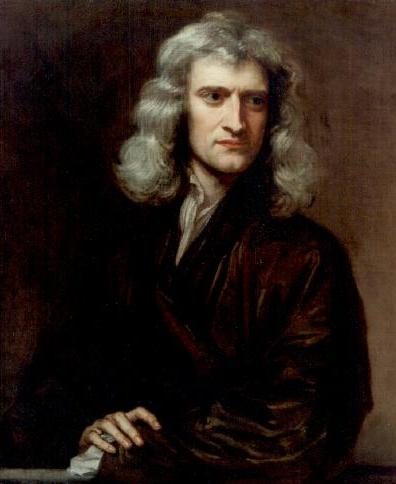
\includegraphics[width=0.24\textwidth]{img/chap0/IsaacNewton.jpg}
  %\end{center}
%\vspace{-20pt}  
\caption{Isaac Newton in 1689}
%\vspace{-10pt}
\end{wrapfigure}

A good speaker will often begin a talk with an outline of what will be discussed in the talk. In the same way, it is incumbent upon the author of a textbook to give the reader the big picture of the subject of the textbook. That is the purpose of this brief chapter.

\paragraph{Calculus is the study of change.} Over time, the population of a city may grow. The price of a stock will fluctuate: sometimes increasing and sometimes decreasing. The cumulative profits of a company may grow or wane. These situations represent changing quantities. We may want to dig deeper and find out how quickly the city is growing or the rate at which a company's stock price or profits are growing. Those are questions that calculus attempts to answer.

\begin{wrapfigure}{R}{0.25\textwidth}
%\vspace{-20pt} 
 \centering
    \includegraphics[width=0.24\textwidth]{img/chap0/GottfriedWilhelmLeibniz.jpg}
  %\end{center}
%\vspace{-20pt}
  \caption{Gottfried Wilhelm Leibniz circa 1695}
%\vspace{-10pt}
\end{wrapfigure}

Calculus was first developed in the late 1600s independently by Sir Isaac Newton\index{Newton, Isaac} and Gottfried Wilhelm Leibniz\index{Leibniz, Gottfried} to help them describe and understand the rules governing the motion of planets and moons. Since then, thousands of other men and women have refined the basic ideas of calculus, developed new techniques to make the calculations easier, and found ways to apply calculus to problems besides planetary motion. Perhaps most importantly, they have used calculus to help understand a wide variety of physical, biological, economic, and social phenomena and to describe and solve problems in those areas.


Part of the beauty of calculus is that it is based on a few very simple ideas. Part of the power of calculus is that these simple ideas can help us understand, describe, and solve problems in a variety of fields.

\section{Two Problems}
\label{sec:twoproblems}

Calculus is the study of two seemingly different questions that are actually inverses of each other.
\begin{enumerate}
    \item What is the {\bf rate of change}\index{Rate of change} of a function?
    \item What is the {\bf accumulation}\index{Accumulation} of a function?
\end{enumerate}
Geometrically, these questions can be visualized as the {\bf slope of a curve}\index{Slope!curve} and the {\bf area under a curve}\index{Area!under a curve}, respectively, as seen in Figure \ref{fig:0-1}. We start with these pictures because a conceptual understanding of calculus (and really, all of mathematics), and not merely as a set of rules and procedures, is crucial to understanding the content of this course and being able to apply it to real-world problems, perhaps even in novel ways.

\begin{figure}[h!]
    \centering
    \begin{subfigure}[b]{0.45\textwidth}
        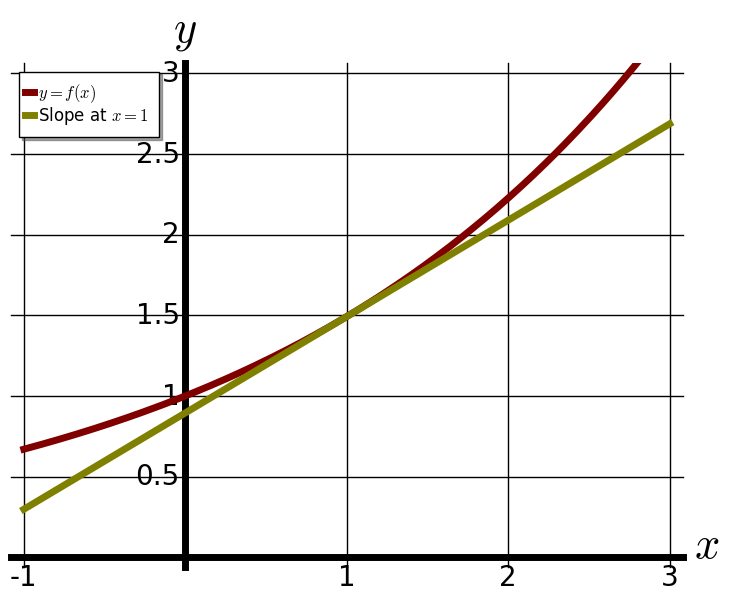
\includegraphics[width=\textwidth]{img/chap0/ex0-1.png}
        \caption{Slope of a Curve at a Point}
        \label{fig:0slope}
    \end{subfigure}
    ~ %add desired spacing between images, e. g. ~, \quad, \qquad, \hfill etc.
    \begin{subfigure}[b]{0.45\textwidth}
        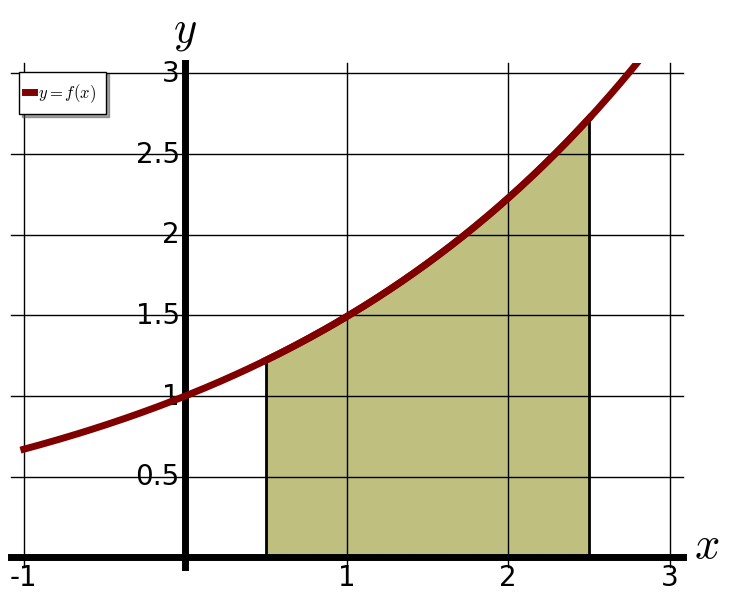
\includegraphics[width=\textwidth]{img/chap0/ex0-2.png}
        \caption{Area Under a Curve over an Interval}
        \label{fig:0area}
    \end{subfigure}
    \caption{Visualizing the Two Problems of Calculus}\label{fig:0-1}
\end{figure}

In this book, we will unpack these two problems and two pictures and show how they are useful to business, economics, finance, the social sciences, and the life sciences. We will take a data-driven and a problem-solving approach to this course, working with real and realistic data. Yes, all of calculus is derived from understanding those two pictures. Study those two pictures again.

Let's consider a pair of examples to illustrate these two concepts.

\begin{example}
Suppose that you're paid $y$ dollars for working $x$ hours. A graph of the relationship between the amount of time you work (in hours) and your pay (in dollars) is in Figure \ref{fig:0-rate}. The slope of the line is your hourly pay rate. In this case, the slope of the curve and the rate of change of the function is \$15 per hour.
\begin{figure}[h!]
\centering
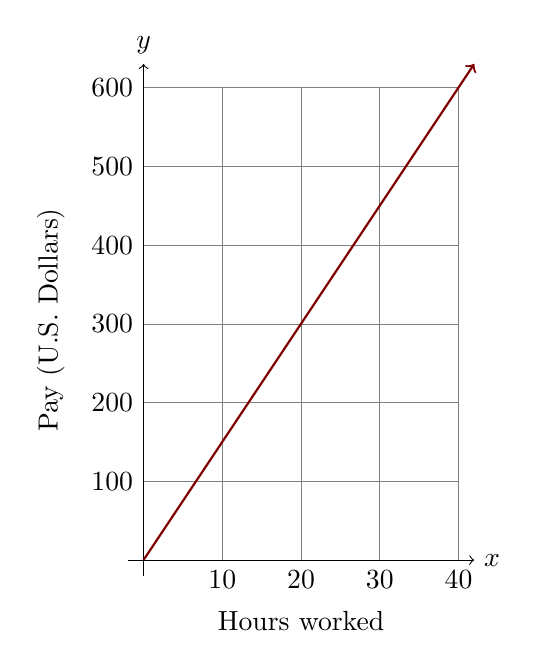
\begin{tikzpicture}[scale=0.1]
    % grid
    \draw[step=10, very thin, gray] (0, 0) grid (40, 60);

    % axes
    \draw[->] (-2,0) -- coordinate (x axis mid) (42,0) node[right] {$x$};
    \draw[->] (0,-2) -- coordinate (y axis mid) (0,63) node[above] {$y$};

    % ticks
    \foreach \x in {10, 20, ..., 40}
     		\draw (\x,1pt) -- (\x,-3pt)
			node[anchor=north] {\x};
    	\foreach \y in {100, 200, ..., 600}
     		\draw (1pt,\y/10) -- (-3pt,\y/10) 
     			node[anchor=east] {\y}; 

    % labels
    \node[below = 15] at (x axis mid) {Hours worked};
	\node[rotate=90, above = 25] at (y axis mid) {Pay (U.S.\ Dollars)};

    % plot 
    \draw[->, thick, color=aldRed] (0, 0) -- (42, 63);
    
    % legend

\end{tikzpicture}
\caption{Pay as a function of time worked.}
\label{fig:0-rate}
\end{figure}
\end{example}

\begin{example}
Suppose that $t$ hours after a snowstorm starts, the snowfall rate is $r(t)$ inches per hour. The shaded area represents the total accumulation of the snow during the storm.
\end{example}

\section{Problem Solving}
\label{sec:polya}

One day when my wife was pregnant with our second child, she was lying down on the couch with a bit of nausea, which is not uncommon in the first trimester. I offered her a ginger candy, which helps to alleviate nausea. Our son, who was a clever two years old at the time asked me, ``Pwease I have ginger candy?" I replied, ``No, you can't have ginger candy. It's for mommy. Mommy's tummy hurts." My son sat for a minute thinking. After a moment, he said. ``My tummy hurts. Pwease I have ginger candy?" He still didn't get the candy; we don't reward dishonesty, but it was a humorous example of problem solving.

Have you ever looked at a math problem and said to yourself, ``I don't know where to start!" No matter how you answered that question, this section will offer some tips.

One often thinks of the study of a mathematical subject as mere rote memorization of formulas and step-by-step procedures. On the contrary, the approach that mathematicians take to the subject is much more creative. We see mathematics as a way to apply abstract concepts to solve problems. Often there is just one correct answer. Often, however, the ``correct" or ``best" answer may be impossible to find, so we are instead interested in a solution that would be considered ``good," ``plausible," or ``reasonable." That is the approach that will drive much of the content of this textbook. In short, one of our objectives is to retrain the way you view mathematics: it's not about knowing or not knowing the answer, it's about figuring out a solution. This textbook is not a book to tell you what to think, but how to think about quantitative problem solving.

In light of this, we introduce a well-known problem-solving process and thoughts on how to implement it in practice. In his famous book {\em How to Solve It}, mathematician George P\'{o}lya \index{P\'{o}lya, George} described his problem-solving process in four steps, which we have modified to follow the acronym ``C.O.P.E."
% [Picture of Polya]
\begin{enumerate}
\item {\bf Comprehend} (Understand) the problem.
\begin{itemize}
    \item {\bf What is the problem asking?}
    \item It is impossible to solve a problem without this step, but it is often skipped.
    \item Read and understand the instructions if there are any.
    \item Read the problem over and over until you understand.
    \item Look up words and symbols you don't understand.
    \item Ask yourself and answer the following questions:
    \begin{itemize}
        \item Is the problem assuming that I know something that I don't?
        \item What knowledge gaps must I fill in order to really understand the problem?
        \item Is there enough information given to solve the problem?
        \item Do I need to look up information for the problem?
        \item Is there any irrelevant information that can be ignored?
        \item Do I need to make any assumptions? If so, are these assumptions reasonable?
        \end{itemize}
    \item It may help to draw a picture or diagram.
    \item It may help to simplify the problem, i.e., work with a simpler ``toy'' problem.
    \item Study examples similar to the problem.
    \item It may help to compare the problem to a similar one.
    \item Be patient with yourself. Sufficient understanding may take time.
    \item What is a range of plausible solutions?
    \item Often there is more than one level of comprehension to a problem or concept. A deeper understanding of a problem or concept results in a better or more advanced solution to the problem.
    \item You may obtain a deeper understanding of the problem by pursuing the next step: ``Observe.''
\end{itemize}
\item {\bf Observe} the information and applicable tools and devise a plan.
\begin{itemize}
    \item {\bf What information is given in the problem and what tools do you have that apply?}
    \item ``Look" around. What (mathematical or other) tools, results, theorems, algorithms, etc.\ apply in this situation, based on the information given?
    \item If you studied examples similar to the problem, do the same tools, results, theorems, or algorithms apply in this case? Why or why not?
    \item Here are some ideas to work with the information.
    \begin{itemize}
        \item Define variables to describe components of the problem and solution. Consider units.
        \item Express the information we have mathematically.
        \item Draw a picture or diagram. Label the picture with variables, numbers, etc.
        \item Make a chart or list or plot some of the data or information.
        \item Experiment. Play with the problem and the math until something works.
        \item Guess and check: Trial and error helps to develop intuition.
        \item Be systematic. Use an organized method to check all cases.
        \item Look for patterns.
        \item Work backwards.
        \item Look for counterexamples.
        \item Divide and conquer. Split the problem up into pieces and solve the individual pieces.
    \end{itemize}
\end{itemize}
\item {\bf Proceed} with the plan and get a solution.
\begin{itemize}
    \item {\bf It often helps to work out a solution on scratch paper first.}
    \item {\bf Make your solution easy to follow for yourself and others.}
    \item Check your work at each step.
    \item If you get stuck or the solution doesn't work, go back to the planning stage and try something else. Thomas Edison tested thousands of designs before developing a practical working lightbulb.
    \item Think about the problem during otherwise unproductive times such as when waiting in line, walking, driving, or falling asleep.
    \item When stuck, take a break and let your brain work on the problem subconsciously.
    \item Be patient. It may take a while for the solution to ``click."
    \item Work on the solution on scratch paper, and carefully write up your solution when you've solved it. The solution must clearly communicate the problem that is being solved and the solution itself. Your solution will be read by others and your future self.
\end{itemize}
\item {\bf Evaluate} (in the sense of ``Reflect on'') your solution and check your work.
\begin{itemize}
    \item (1) {\bf Does the solution answer the question or solve the problem?}
    \item (2) {\bf Does the solution make sense?}
    \item Skipping this step often results in ``stupid" mistakes that are easy to catch.
    \item Are there any obvious errors or contradictions?
    \item Does the solution fit within a range of plausible solutions?
    \item Is there another, independent approach to validate the solution or confirm that it is plausible?
    \item Do the units make sense?
    \item Check your work. This is why organized solutions are important.
    \item Proofread any written work, ideally at least a day after you wrote it.
\end{itemize}
\item {\bf Extend} (Generalize) the solution or problem and reflect.
\begin{itemize}
    \item Is there another, possibly easier, way to solve the problem?
    \item Can you generalize the problem?
    \item Would you do something different to improve the solution?
\end{itemize}
\end{enumerate}

My charge to you, the student of calculus, is to keep the C.O.P.E.\ problem solving method in mind throughout your course. {\bf Comprehension} will often involve reviewing earlier chapters and sections, looking up content in the index, and in many cases, and reviewing material from earlier courses such as algebra. Be patient with yourself. When {\bf observing} what tools apply, again, review of the text may be likely. Just as a hammer doesn't work well to put a nut on a bolt, make sure that the right mathematical tool applies to the problem at hand. If not, then don't use the tool. Be patient with yourself. When {\bf proceeding} with the solution, keep in mind that the point of writing up a solution is to clearly communicate the solution to the intended audience. That audience may be your future self. Write  your solution so as to make it impossible to misunderstand. Be sure that all graphics are clear and labeled and that all variables are defined. Be patient with yourself. When {\bf evaluating} your solution, be critical with yourself. Expect there to be something wrong and scrutinize each step. Finally, if you approach this course with the intent to understand the concepts and the pictures behind each concept, then you will be in an excellent position to {\bf extend} any solution and apply it in powerful ways in your particular field of study. I hope you enjoy this book and this course and that you find it useful throughout your life.


\subsection{Exercises}
\label{0-3-exercises}

\begin{enumerate}

    \item Give an example of a rate of change that you have seen in your life (other than one of the examples in this chapter).

    \item Give an example of an accumulation of a rate that you have seen in your life (other than one of the examples in this chapter).

    \item Why would we call a solution to a problem ``plausible," ``good," or ``reasonable," rathen than ``correct?"

    \item Give an example of a time when you used the C.O.P.E.\ problem solving process in your life.

    \item What does it mean to have a conceptual understanding of mathematical idea?

    \item Why is it important to understand a mathematical principle conceptually, rather than merely memorizing rote procedures?

\end{enumerate}

% {\bf Problem solving strategy}
%
% \begin{enumerate}
% \item Identify changing quantities, and then carefully and clearly define descriptive variables to represent those quantities. When appropriate, sketch a picture or define a coordinate system.
% \item Carefully read the problem to identify important information. Look for information giving values for the variables, or values for parts of the functional model, like slope and initial value.
% \item Carefully read the problem to identify what we are trying to find, identify, solve, or interpret.
% \item Identify a solution pathway from the provided information to what we are trying to find. Often this will involve checking and tracking units, building a table or even finding a formula for the function being used to model the problem.
% \item When needed, find a formula for the function.
% \item Solve or evaluate using the formula you found for the desired quantities.
% \item Reflect on whether your answer is reasonable for the given situation and whether it makes sense mathematically.
% \item Clearly convey your result using appropriate units, and answer in full sentences when appropriate.
% \end{enumerate}

    \chapter{Models, Graphs, and Functions}
\label{ch:models}

%\section{Review of Algebra}
\label{sec:review}

\section{What is a Function?}
\label{sec:functions}
% To do: graphs, images, Excel/LibreOffice Calc spreadsheets.

\subsection{Function Concepts}

The natural world is full of relationships between quantities that change. When we see these
relationships, it is natural for us to ask ``If I know one quantity, can I then determine the other?" This establishes the idea of an input quantity, or {\bf independent variable}\index{Variable!independent}, and a corresponding output quantity, or {\bf dependent variable}\index{Variable!dependent}. From this, we get the notion of a functional relationship in which the output can be determined from the input.

For some quantities, like height and age, there are certainly relationships between these
quantities. Given a specific person and any age, it is easy enough to determine their height, but if we tried to reverse that relationship and determine age from a given height, that would be problematic, since most people maintain the same height for many years.

\begin{definition}
A {\bf function}\index{Function} is a rule for a relationship between an {\bf input} (or {\bf independent}) quantity and an {\bf output} (or {\bf dependent}) quantity in which each input value uniquely determines one output value. We say ``the output is a function of the input."
\end{definition}

\begin{example}
\label{ex:height}
In the height and age example above, is height a function of age? Is age a function of height?

\begin{solution} In the height and age example above, it would be correct to say that height is a function of age, since each age uniquely determines a height. You cannot have two different heights at any one instant in time.

However, age is not a function of height, since one height input might correspond with more than one output age. Once you have stopped growing, your height essentially remains constant for the rest of your life.
\end{solution}\end{example}

\subsection{Representing Functions}

Functions can be represented in many ways:
    \begin{multicols}{2}
    \begin{enumerate}
        \item A description of a relationship between variables,
        \item Tables of values,
        \item Graphs,
        \item Formulas,
        \item An action verb, and
        \item A black box with input and output.
    \end{enumerate}
    \end{multicols}
Example \ref{ex:height} represented a function in words, but it will be convenient to streamline the discussion of a function. To that end, we introduce notation of functions.

\paragraph{Function Notation.}

To simplify writing out expressions and equations involving functions, a simplified notation is often used. We also use descriptive variables to help us remember the meaning of the quantities in the problem.

Rather than write ``height is a function of age'', we could use the descriptive variable $h$ to represent height and we could use the descriptive variable $a$ to represent age.

If we name the function $f$ we could write ``height is a function of age" as ``$h$ is $f$ of $a$," or more simply:
$$h = f(a) \enspace .$$

We could instead name the function $h$ and write $h(a)$, which is read ``$h$ of $a$."

We can use any variable to name the function; the notation $h(a)$ shows us that $h$ depends on $a$. The value ``$a$'' must be put into the function ``$h$'' to get a result.

\begin{remark}
Be careful! The parentheses indicate that age is the input into the function. Do not confuse these parentheses with multiplication!
\end{remark}

\begin{example}
A function $N = f(y)$ gives the number of police officers, $N$, in a town in year $y$. What does $f(2005) = 300$ tell us?

\begin{solution} When we read $f(2005) = 300$, we see the input quantity is 2005, which is a value for the input quantity of the function: the year ($y$). The output value is $300$, the number of police officers ($N$), a value for the output quantity. Remember $N=f(y)$. This tells us that in the year 2005 there were 300 police officers in the town.
\end{solution}\end{example}

\paragraph{Tables as Functions.}

A table lists the input and corresponding output values of a function.

In some cases, these values represent everything we know about the relationship, while in other cases the table is simply providing us a few select values from a more complete relationship.

Table \ref{tab:function} below represents the age of a child in years and his
corresponding height. This represents just some of the data available
for the age and height of the child.

\begin{table}[ht!]
\begin{centering}
\begin{tabular}{l*{7}{r}}
\toprule
{\bf (Input:)} $a$, age (years) & 4 & 5 & 6 & 7 & 8 & 9 & 10\\
\midrule
{\bf (Output:)} $h$, height (inches) & 40 & 42 & 44 & 47 & 50 & 52 & 54\\
\bottomrule
\end{tabular}
\caption{Tabulating height as a function of age for a child.}
\label{tab:function}
\end{centering}
\end{table}
From this, we can create equations such as $h(6) = 44$, meaning that when the child was 6 years old, he was 44 inches tall.


\begin{example}

Which of these tables define a function (if any)?

\begin{center}
\begin{tabular}{ccc}
\multicolumn{2}{c}{Table A.}\\
\toprule
{\bf Input} & {\bf Output}\\
\toprule
2 & 1 \\
\midrule
5 & 3 \\
\midrule
8 & 6 \\
\bottomrule
\end{tabular}
\quad
\begin{tabular}{ccc}
\multicolumn{2}{c}{Table B.}\\
\toprule
{\bf Input} & {\bf Output}\\
\toprule
$-3$ & 5 \\
\midrule
0 & 1 \\
\midrule
4 & 5 \\
\bottomrule
\end{tabular}
\quad
\begin{tabular}{ccc}
\multicolumn{2}{c}{Table C.}\\
\toprule
{\bf Input} & {\bf Output}\\
\toprule
1 & 0 \\
\midrule
5 & 2 \\
\midrule
5 & 4 \\
\bottomrule
\end{tabular}
\end{center}

\begin{solution} Tables A and B define functions. In both tables, each input corresponds to exactly one output. Table C does not define a function since the input value of 5 corresponds with two different
output values: 2 and 4.
\end{solution}\end{example}



\paragraph{Graphs as Functions}

A function can often be represented as a {\bf graph}\index{Graph}, a set of {\bf points}\index{Point} plotted on {\bf coordinate axes}\index{Coordinate axes}: the {\bf horizontal axis}\index{Axis!horizontal} and the {\bf vertical axis}\index{Axis!vertical}. By convention, graphs are typically created with the input quantity along the horizontal axis and the output quantity along the vertical axis.

Points on the graph are represented by ordered pairs of the form $(a, b)$. Beginning at the {\bf origin}\index{Origin} (the point $(0,0)$), you move $a$ units to the left and $b$ units up to arrive at the point $(a, b)$. If $a<0$, then movement is to the left and if $b<0$, then movement is down.

\begin{wrapfigure}{r}{0.3\textwidth}
    \centering
    \vspace{-12pt}
    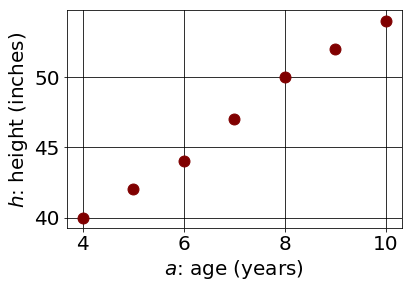
\includegraphics[width=0.3\textwidth]{img/chap1/sec1-2/table1-1.png}\\
    \caption{A plot of height data.}
    \label{fig:heightplot}
\end{wrapfigure}
The horizontal and vertical axes are typically called the {\bf $x$-axis}\index{$x$-axis} and the {\bf $y$-axis}\index{$y$-axis}, but these axes can be labeled with any variable name, not just $x$ and $y$. We say $y$ is a function of $x$, or $y = f(x)$ when the function is named $f$. The point $(a, b)$ lies on the graph of the function $f$ if and only if $f(a)=b$.

As an example, Figure \ref{fig:heightplot} is a plot of the data from Table \ref{tab:function}.

\begin{example}
\label{ex:1-2-graphs}
Which of these graphs defines a function $y=f(x)$?
\begin{figure}[!ht]
    \centering
    \begin{subfigure}[b]{0.3\textwidth}
        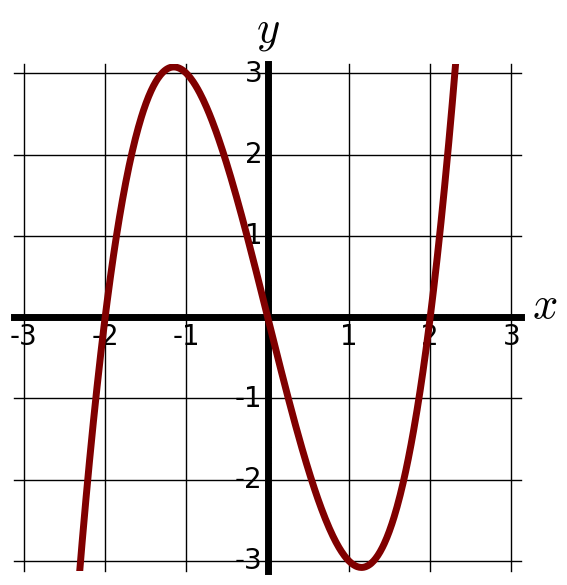
\includegraphics[width=\textwidth]{img/chap1/sec1-2/ex114a.png}
        \caption{Graph A}
    \end{subfigure}
    ~
    \begin{subfigure}[b]{0.3\textwidth}
        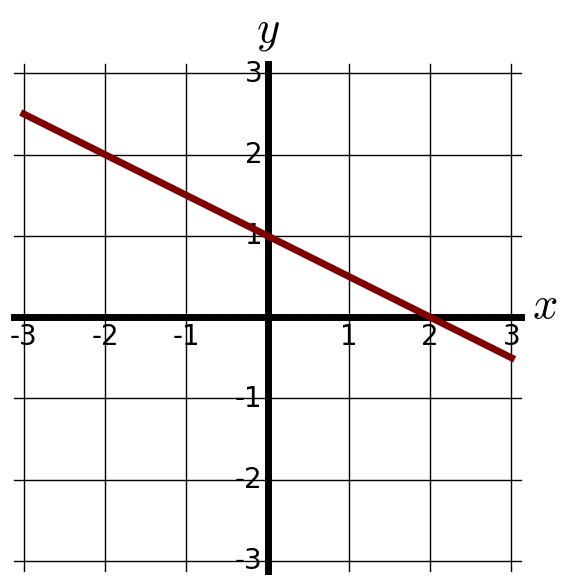
\includegraphics[width=\textwidth]{img/chap1/sec1-2/ex114b.png}
        \caption{Graph B}
    \end{subfigure}
    ~
    \begin{subfigure}[b]{0.3\textwidth}
        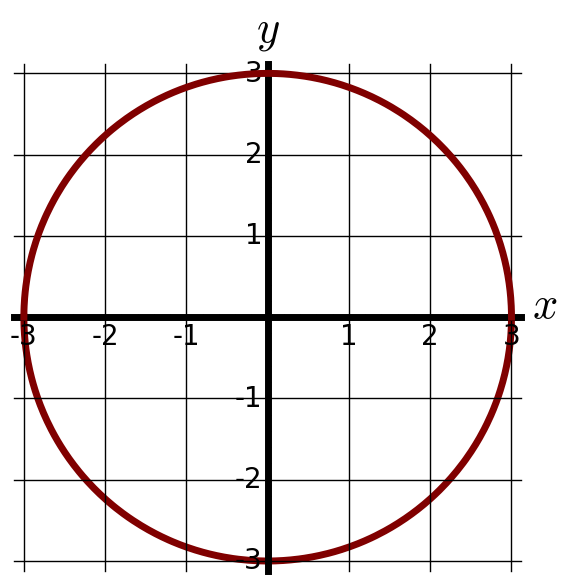
\includegraphics[width=\textwidth]{img/chap1/sec1-2/ex114c.png}
        \caption{Graph C}
    \end{subfigure}
\end{figure}

\begin{solution} Looking at the graphs above, Graphs A and B define a function $y=f(x)$, since for each input value along the horizontal ($x$) axis, there is exactly one corresponding output value, determined by the $y$-value of the graph. Graph C does not define a function $y=f(x)$ since some input values, such as
$x=2$, correspond with more than one output value.
\end{solution}\end{example}

\begin{wrapfigure}{r}{0.3\textwidth}
    \centering
    \vspace{-12pt}
    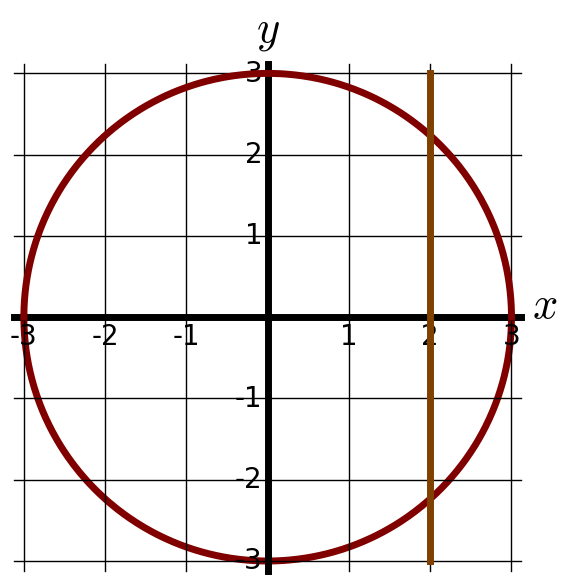
\includegraphics[width=0.3\textwidth]{img/chap1/sec1-2/fig115.png}\\
    \caption{A graph failing the vertical line test.}
    \label{fig:1-2-115}
\end{wrapfigure}
The \textbf{vertical line test}\index{Vertical line test} is an easy way to determine whether a graph defines a function or not. Imagine drawing vertical lines through the graph. Since a function has exactly one output for every input, if there is a vertical line that would cross the graph more than once, then the graph does not define a function.

Figure \ref{fig:1-2-115} illustrates how Graph C from Example \ref{ex:1-2-graphs} fails the vertical line test. The vertical line $x=2$ (in gold) intersects Graph C (in maroon) at two points; there are two outputs for for the input $x=2$.

\paragraph{Formulas as Functions}

When possible, it is very convenient to define relationships between quantities using a formula. If it is possible to express the output as a formula involving the input quantity, then we can define a function.

\begin{example}
Express the relationship $2N + 6p = 12$ as a function $p = f(N)$ if possible.

\begin{solution} To express the relationship in this form, we need to be able to write
the relationship where $p$ is a function of $N$, which means
writing it as $p = $ something involving $N$, or $p$ in terms of $N$. We proceed using algebra.

\begin{align*}
&2N + 6p = 12& &\mbox{Subtract $2N$ from both sides.}\\
&6p = 12 - 2N& &\mbox{Divide both sides by 6 and simplify.}\\
&p = \frac{12-2N}{6}& & \\
&p = \frac{12}{6} - \frac{2N}{6} & &\\
&p = 2 - \frac{1}{3}N & &
\end{align*}
We can now express $p$ as a function of $N$:
$$p = f(N) = 2 - \frac{1}{3}N \enspace .$$
\end{solution}\end{example}

It is important to note that not every relationship can be expressed as a function with a formula. Consider the examples of the boy's height as a function of age in Table \ref{tab:function} or a company's stock price as a function of time. Neither situation allows one to define the relationship using a formula precisely, yet we still may want to analyze aspects of these relationships using tools of calculus. The rest of the chapter will introduce us to some tools to help us with that.

Note the important feature of an equation written as a function is that the output value can be determined directly from the input by doing evaluations. This allows the relationship to act as a magic box that takes an input, processes it, and returns an output. Modern technology and computers rely on these functional relationships, since the evaluation of the function can be programmed.

\subsection{Evaluating Functions.}

The fundamental use of a function is to {\bf evaluate} the function: ``plugging in" some number into the function, or more precisely, to determine the corresponding output for a given input. In other words, we substitute or replace the input variable of the function with the input value. Evaluating will always produce one result, since each input of a function corresponds to exactly one output. We can evaluate a function from a table, graph, or formula.

Another related use is to determine the input or inputs of a function, given an output of the function. This is called {\bf solving} an equation and could produce more than one solution, since different inputs can produce the same output.

\begin{remark}
The concepts of evaluating and solving often get confused. When we use the word {\em solve}, we will be {\em solving a problem} or {\em solving an equation for an unknown quantity or variable}. It does not make sense to solve a function, since a function is merely a mathematical expression and not an equation.
\end{remark}

\begin{example}
Let $Q=g(n)$ and use the table shown.

\begin{center}
    \begin{tabular}{*{6}{l}}
    \multicolumn{6}{c}{$Q = g(n)$ as a table.}\tabularnewline
    \toprule
    $n$ & 1 & 2 & 3 & 4 & 5 \tabularnewline
    \midrule
    $Q$ & 8 & 6 & 7 & 6 & 8 \tabularnewline
    \bottomrule
    \end{tabular}
\end{center}

    \begin{itemize}
        \item[(a)] Evaluate $g(3)$.

\begin{solution} Evaluating $g(3)$, read ``$g$ of 3,'' means that we need to determine the output value, $Q$, of the function $g$ given the input value of $n=3$. Looking at the table, we see the output corresponding to $n=3$ is $Q=7$, allowing us to conclude $g(3) = 7$.
\end{solution}
    \item[(b)] Solve $g(n) = 6$ for $n$.

    \begin{solution} Solving $g(n) = 6$ means we need to determine what input values, $n$, produce an output value of 6. Looking at the table we see there are two solutions: $n = 2$ and $n = 4$.

      When we evaluate $g(n)$ at 2, our output is $Q = 6$.

      When we evaluate $g(n)$ at 4, our output is also $Q= 6$.
    \end{solution}
    \end{itemize}
\end{example}

Evaluating a function using a graph requires taking the given input and using the graph to look up the corresponding output. Solving a function equation using a graph requires taking the given output and looking on the graph to determine the corresponding input.

\begin{minipage}{0.65\textwidth}
\begin{example}
Consider the graph of a function $f(x)$ to the right.

    \begin{itemize}

        \item[(a)] Evaluate $f(2)$.

        \begin{solution} To evaluate $f(2)$, we find the input of $x=2$ on the horizontal ($x$) axis. Moving up to the graph gives the point $(2, 1)$, giving an output of $y=1$. Therefore, $f(2) = 1$.
\end{solution}
        \item[(b)] Solve $f(x) = 4$ for $x$.

        \begin{solution} To solve $f(x) = 4$, we find the value 4 on the vertical ($y$) axis because if $f(x) = 4$ then 4 is the output. Moving horizontally across the graph gives two points with the output of 4: $(-1,4)$ and $(3,4)$. These give the two solutions to $f(x) = 4$: $x = -1$ or $x = 3$.

        This means $f(-1)=4$ and $f(3)=4$, or when the input is $-1$ or 3, the output is 4.
        \end{solution}
    \end{itemize}

\end{example}
 \end{minipage}
 \begin{minipage}{0.3\textwidth}
%\begin{figure}
 %{wrapfigure}{r}{0.3\textwidth}
 %\begin{floatingfigure}{0.3\textwidth}
%     \centering
     %\vspace{-32pt}
     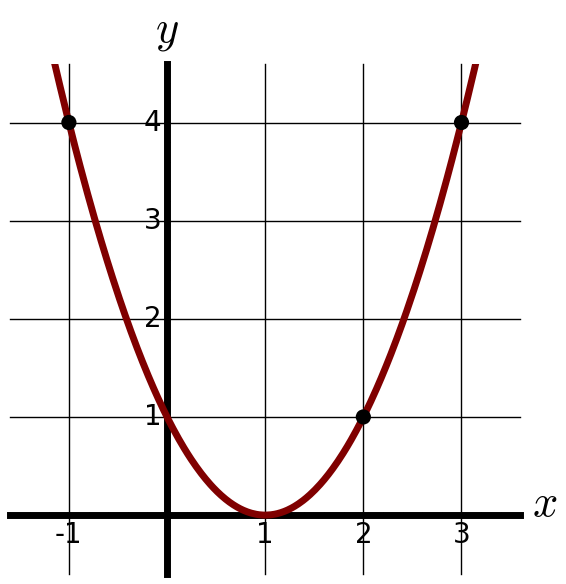
\includegraphics[width=\textwidth]{img/chap1/sec1-2/ex117.png}
 %\end{wrapfigure}
 %\end{floatingfigure}
%\end{figure}
\end{minipage}

\begin{example}
Let $k(t) = t^3 + 2$.
    \begin{itemize}
        \item[(a)] Evaluate $k(2)$.

        \begin{solution} To evaluate $k(2)$, we replace $t$ with 2 in the expression $t^3+2$, then simplify.
        \begin{align*}
            k(2) &= 2^3 + 2 \\
            &= 8 + 2 \\
            &= 10
        \end{align*}
        So $k(2) = 10$.
        \end{solution}
        \item[(b)] Solve $k(t) = 1$ for $t$.

        \begin{solution} To solve $k(t) = 1$, we set the formula for $k(t)$ equal to 1, and solve for the input value that will produce that output.
        \begin{align*}
            k(t)    &=  1 & &\mbox{Substitute the original formula } k(t) = t^3 + 2.\\
            t^3 + 2 &=  1 & &\mbox{Subtract 2 from each side}. \\
            t^3     &= -1 & &\mbox{Evaluate the cube root of each side.}\\
            t       &= \sqrt[3]{-1} = -1& &
        \end{align*}

When solving an equation using formulas, you can check your answer by using your solution in the original equation to see if your calculated answer is correct.

To check our work, we want to know if $k(t)=1$ is a true statement when $t=-1$.
    \begin{align*}
        k(-1) &= (-1)^3 + 2 \\
              &= -1 + 2 \\
              &= 1 \enspace ,
          \end{align*}
which was the desired result.
\end{solution}
    \end{itemize}
\end{example}


\subsection{Cost, Revenue, Profit, and Demand}
\label{ssec:cost}
Suppose that your club wants to raise funds by selling T-shirts. The screen printing shop that will make the shirts will charge your club \$50 to cover overhead costs and \$5 per shirt for the shirts themselves. You decide to charge \$15 per shirt. Some questions naturally arise. How many shirts need to be sold to {\bf break even}? How much {\bf profit} can be expected?

We can describe situations such as this with functions. The {\bf total cost}\index{Cost!total} to produce these shirts combines {\bf fixed costs}\index{Cost!fixed} and {\bf variable costs}\index{Cost!variable}. The fixed costs are also called {\bf overhead costs} and do not depend on the number of T-shirts made, while the variable costs are the per item cost. If $n$ is the number of T-shirts the screen printing shop will make, $F(n)$ is the fixed costs and $V(n)$ is the variable costs, then the {\bf cost function}\index{Function!cost} to produce $n$ T-shirts is
\begin{align*}
\mbox{ total cost } &= \mbox{ fixed costs } + \mbox{ variable costs}\\
C(n) &= F(n) + V(n)\\
&= \$50 + \left(\$5\mbox{ per shirt}\right)\left(n\mbox{ shirts}\right)\\
&= 50 + 5n \mbox{ dollars}
\end{align*}

If you sell each shirt for \$15 and you sell $n$ shirts, then your {\bf revenue}\index{Revenue} from selling $n$ shirts will be $15n$ dollars. This is your {\bf revenue function}\index{Function!revenue}: $R(n)=15n$ dollars.

Finally, the {\bf profit}\index{Profit} that your club will earn from selling $n$ shirts is the revenue minus the total costs. If $P(n)$ is the profit from selling $n$ items, then the {\bf profit function}\index{Function!profit} is
$$P(n) = R(n) - C(n) \enspace .$$
In this example, we have
\begin{align*}
P(n) &= R(n) - C(n)\\
&= 15n - (50 + 5n) \mbox{ dollars}\\
&= 15n - 50 - 5n \mbox{ dollars}\\
&= 10n - 50 \mbox{ dollars}
\end{align*}
\begin{example}
Consider the T-shirt scenario above.
    \begin{itemize}
        \item[(a)] What is the profit from selling 30 shirts?

        \begin{solution} $P(30) = 10\cdot 30 - 50 = 300 - 50 = \$250$.

        If you sell 30 T-shirts, then you profit \$250.
        \end{solution}

        \item[(b)] What is the profit from selling 3 shirts?

        \begin{solution} $P(3) = 10\cdot 3 - 50 = 30-50 = \$(-20)$.

        If you only sell 3 T-shirts, then you lose \$20; your profit is negative.
        \end{solution}
        \item[(c)] What is the profit from selling 0 shirts?

        \begin{solution} $P(0) = 10\cdot 0 - 50 = 0-50 = \$(-50)$.

        If you don't sell any T-shirts, then you lose \$50; your profit is negative.
        \end{solution}
    \end{itemize}
\end{example}
The {\bf break-even point}\index{Break-even point} in this context is the minimum number of T-shirts that must be sold in order to have a profit of at least \$0. How do we find this? If our profit is \$0, then we turn that sentence into a mathematical equation and solve for the number of shirts. The profit from selling $n$ shirts is $P(n)$, ``is" is ``$=$", and $0$ is $0$.
\begin{align*}
P(n) &= 0 \\
10n-50 &= 0\\
10n &= 50 \\
n &= \frac{50}{10} = 5
\end{align*}
So you need to sell at least five T-shirts in order to break even.

\begin{remark}
Note the distinction between $P(0)$ and $P(n)=0$. $P(0)$ is the profit from selling 0 items, while $P(n)=0$ is an equation whose solution tells you the number of items that must be sold in order to have no profit.
\end{remark}

\begin{definition}
In summary, the {\bf total cost}\index{Cost!total} to produce $n$ items, $C(n)$, is the combination of {\bf fixed costs}\index{Cost!fixed}, $F(n)$, and {\bf variable costs}\index{Cost!variable}, $V(n)$. The fixed costs are also called {\bf overhead costs} and is constant regardless of the number of items made, while the variable costs depend on the number of items being made. So
$$C(n) = F(n) + V(n)\enspace .$$
The {\bf revenue}\index{Revenue} function, $R(n)$ gives the amount of money brought in from selling $n$ items. The difference between revenue and total costs is {\bf profit}\index{Profit} ($P(n)$) from selling $n$ items:
$$ P(n) = R(n) - C(n)\enspace .$$
The {\bf break-even point}\index{Break-even point} is the fewest number of items, $n$, that must be sold in order for $P(n) \geq 0$, in other words, the fewest number of items to guarantee that you won't have negative profit and be losing money.
\end{definition}
\begin{definition}
{\bf Demand}\index{Demand} is the functional relationship between the price $p$ and the quantity $q$ of an item that can be sold (that is demanded). Depending on your situation, you might think of $p$ as a function of $q$, or of $q$ as a function of $p$. If the quantity of an item that is demanded depends on the price it is sold at, then we would write $q = D(p)$.
\end{definition}
\begin{definition}
The {\bf supply}\index{Supply} of an item is the quantity $q$ that is available for sale (that is supplied) at a price $p$. If the supply of an item for sale depends on the price it is sold at, then we would write $q = S(p)$.
\end{definition}
\begin{definition}
\label{def:avgcost}
The {\bf average cost}\index{Cost!average} to produce $n$ items is 
$$A(n) = \frac{C(n)}{n} \enspace .$$
\end{definition}

\begin{example}
Table \ref{tab:1-2-cost} shows the total cost ($C(n)$) of producing $n$ items.
\begin{table}[ht!]
\centering
\begin{tabular}{cc}
\toprule
Items ($n$)	& Cost $C(n)$ \\
\midrule
0	& \$20,000\\
100	& \$35,000\\
200	& \$45,000\\	
300	& \$53,000\\
\bottomrule
\end{tabular}
\caption{Cost to produce $n$ items.}
\label{tab:1-2-cost}
\end{table}
\begin{enumerate}[label=(\alph*)]
    \item What is $F(n)$, the fixed cost for producing $n$ items?

    \begin{solution}
    The fixed cost is $F(n) = C(0) = \$20,000$, the cost even when no items (i.e., when $n=0$ items) are made.
    \end{solution}
    \item When 200 items are made, what is the variable cost?

    \begin{solution}
    The fixed cost is \$20,000, and when 200 items are made, the total cost is $C(200) = \$45,000$. Subtracting the fixed cost, the total variable cost is $V(200) = C(200) - F(n) = C(200) - C(0) = \$45,000 - \$20,000 = \$25,000$.
    \end{solution}
    \item When 200 items are made, what is the average cost?

    \begin{solution}
    The average cost is the total cost divided by the number of items: $A(200) = \frac{C(200)}{200 \mbox{ items}} = \frac{\$45,000}{200\mbox{ items}} = \$225$ per item. So, on average, each item had a cost of \$225.
    \end{solution}    
    
    \item When 200 items are made, what is the average {\bf variable} cost?

    \begin{solution}
    The average variable cost would be the total variable cost divided by the number of items: $\frac{V(200)}{200 \mbox{ items}} = \frac{\$25,000}{200\mbox{ items}} = \$125$ per item. So, on average, each item had a variable cost of \$125.
    \end{solution}
\end{enumerate}

\end{example}

\subsection{Domain and Range.}

One of our main goals in mathematics is to model the real world with mathematical functions. In doing so, it is important to keep in mind the limitations of the models we create. In our most recent example, it wouldn't make sense to sell $-4$ T-shirts or $4.4$ T-shirts. We also wouldn't expect to sell a billion T-shirts for a university club fund raiser. When using a function to describe a real-world scenario, we need to set common sense boundaries for the input and output. Here is another example.

Table \ref{tab:1-tree} shows a relationship between the circumference, $c$, and height, $h$, of a tree as it grows. In this table, we would consider height as a function of circumference: $h = h(c)$.

\begin{table}[ht!]
\begin{centering}
\begin{tabular}{l*{5}{r}}
\toprule
{\bf Circumference:} $c$ (feet) & 1.7 & 2.5 & 5.5 & 8.2 & 13.7\tabularnewline
\midrule
{\bf Height:} $h$ (feet) & 24.5 & 31.0 & 45.2 & 54.6 & 92.1\tabularnewline
\bottomrule
\end{tabular}
\caption{Height of a tree as a function of its circumference.}
\label{tab:1-tree}
\end{centering}
\end{table}
While there is a strong relationship between the two, it would certainly
be ridiculous to talk about a tree with a circumference of $-3$ feet, or a
height of $3000$ feet. When we identify limitations on the inputs and
outputs of a function, we are determining the {\bf domain}\index{Domain} and {\bf range}\index{Range} of the function.

\begin{definition}
The {\bf domain} of a function is the set of possible input values to the function.

The {\bf range} of a function is the set of possible output values of the function.
\end{definition}

\begin{example}
Using Table \ref{tab:1-tree} above, determine a reasonable domain and range of the function $h$.

\begin{solution} We can combine the data provided with additional research and our own reason
to determine an appropriate domain and range of the function $h = h(c)$. For
the domain, it doesn't make sense for the circumference (input) to be negative, so $c \ge 0$. For a maximum circumference, we could make an educated guess at a reasonable value, or
look up that the maximum recorded circumference is about 119
feet\footnote{\url{http://en.wikipedia.org/wiki/Tree}, retrieved July
  19, 2010}. With this information, we would say a reasonable domain is $0\le c \le 119$ feet.

Similarly for the range, if we only consider the tree when the sprout has broken through the ground, it doesn't make sense to have negative heights. The maximum recorded height of a tree could be looked up to be 379 feet, so a reasonable range is $0\le h\le 379$ feet.
\end{solution}\end{example}

\begin{wraptable}{r}{0.4\textwidth}
    \centering
\begin{tabular}{ll}
\toprule
\textbf{Inequality} & \textbf{Interval Notation}\tabularnewline
\midrule
$5\le x \le 10$  & $[5, 10]$\\
$5 <  x \le 10$  & $(5, 10]$\\
$5\le x  <  10$  & $[5, 10)$\\
$5 <  x  <  10$  & $(5, 10)$\\
$x < 10$         & $(-\infty, 10)$\\
$5 \le x$        & $[5, \infty)$\\
All real numbers & $(-\infty, \infty)$ \\
\bottomrule
\end{tabular}
\caption{Interval Notation}
\label{tab:1-interval}
\end{wraptable}
\paragraph{Interval Notation.} A convenient alternative to the notation using inequalities is \textbf{interval notation}\index{Interval notation}, in which intervals of values are referred to by the starting and ending values. Parentheses ``$()$" are used for ``strictly less than,'' and square brackets ``$[]$" are used for ``less than or equal to.'' Since infinity, $\infty$, is not a number, neither $-\infty$ nor $\infty$ are included in the domain and range of a function, so we always use curved parentheses with $\pm\infty$. Table \ref{tab:1-interval} shows how inequalities correspond to interval notation for an arbitrary variable $x$.

To combine two intervals together, we can use the word ``or''. In interval notation, we use the
union\index{Union} symbol, $\cup$, to combine two unconnected intervals together.

\begin{figure}[ht!]
\centering
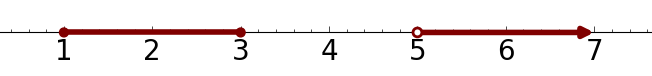
\includegraphics[width=0.5\textwidth]{img/chap1/sec1-2/ex-1-2-11.png}
\caption{A union of intervals.}
\label{fig:1211}
\end{figure}

\begin{example}
Describe the intervals of values shown in Figure \ref{fig:1211} using inequalities and using interval notation.

\begin{solution} To describe the values, $x$, that lie in the intervals shown above
we would say, ``$x$ is a real number greater than or equal to 1 and
less than or equal to 3, or a real number greater than 5.''

As an inequality it is: $1\le x\le 3$ or $x > 5$.

In interval notation: $[1, 3]\cup(5, \infty)$.
\end{solution}\end{example}

\begin{example}
Find the domain of each function.
\begin{itemize}
    \item[(a)] $f(x) = 2\sqrt{x+4}$

    \begin{solution} Since we cannot evaluate the square root of a negative number, we need the inside of the square root to be non-negative. $x+4 \ge 0$ when $x \ge -4$. (Subtract 4 from both sides of the inequality.) Therefore, the domain of $f(x)$ is $[-4, \infty)$.
        \end{solution}
    \item[(b)] $g(x) = \frac{3}{6-3x}$

    \begin{solution} We cannot divide by zero, so we need the denominator to be non-zero. Solving $6-3x = 0$ for $x$, we have $x = 2$, so we must exclude 2 from the domain. Therefore, the domain of $g(x)$ is $(-\infty, 2)\cup(2, \infty)$.
        \end{solution}
\end{itemize}

\end{example}


\subsection{Exercises}
\label{1-2-exercises}

\begin{enumerate}
\item The amount of garbage, $G$, produced by a city with population
  $p$ is given by $G=f(p)$. $G$ is measured in tons per week, and
  $p$ is measured in thousands of people.

  \begin{enumerate}
  \item The town of Tola has a population of 40,000 and produces 13 tons of
    garbage each week. Express this information in terms of the function
    $f$.
  \item Explain the meaning of the statement $f(5)=2$.
  \end{enumerate}

\item The number of cubic yards of dirt, $D$, needed to cover a garden
  with area $a$ square feet is given by $D=g(a)$.

  \begin{enumerate}
  \item A garden with area 5000 ft\textsuperscript{2} requires 50 cubic
    yards of dirt. Express this information in terms of the function
    $g$.
  \item Explain the meaning of the statement $g(100)=1$.
  \end{enumerate}

\item Let $n(t)$ be the number of subscribers to a YouTube channel $t$ years after 2005.
  Explain the meaning of each statement.
  \begin{enumerate}
    \item $n(5) = 300$
    \item $n(10) = 4000$
\end{enumerate}

\item
  Let $p(t)$ be the stock price, in dollars, of Valvoline (VVV) $t$ years after its Initial Public Offering (IPO) on September 23, 2016. Explain the meaning of each statement.
  \begin{enumerate}
    \item $p(0) = 23.10$
    \item $p(1) = 23.27$
    \item $p(2) = 21.47$
\end{enumerate}

\item  Select all of the following graphs which represent $y$ as a function of $x$.

\begin{center}
\begin{tabular}{ccc}
Graph A. & Graph B. & Graph C. \\
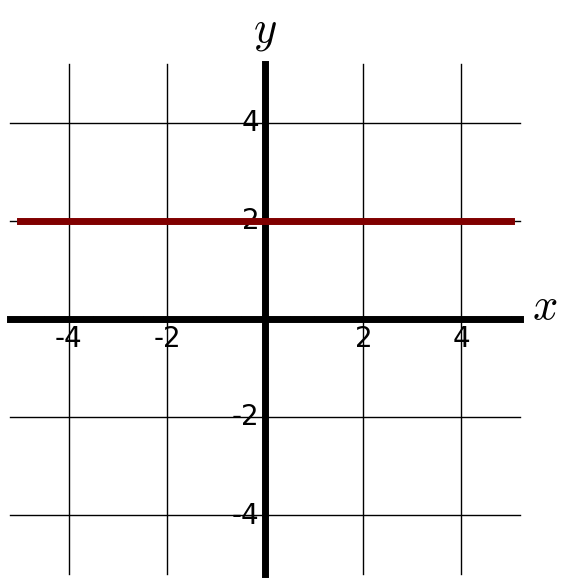
\includegraphics[width=0.2\textwidth]{img/chap1/sec1-2/prob3a.png} & 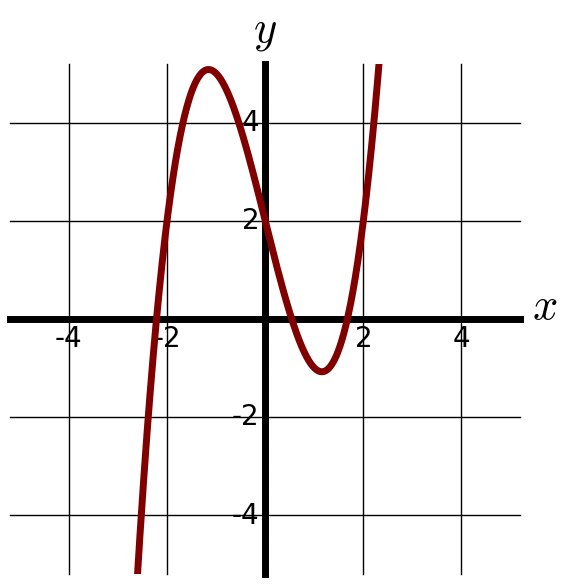
\includegraphics[width=0.2\textwidth]{img/chap1/sec1-2/prob3b.png} &
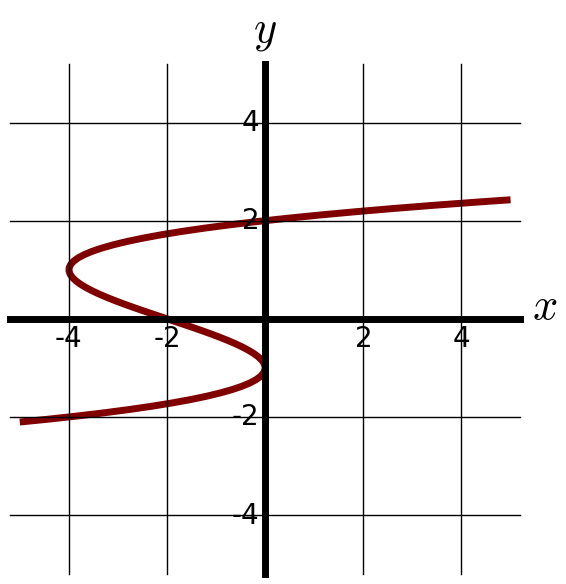
\includegraphics[width=0.2\textwidth]{img/chap1/sec1-2/prob3c.png} \\
\midrule
Graph D. & Graph E. & Graph F. \\
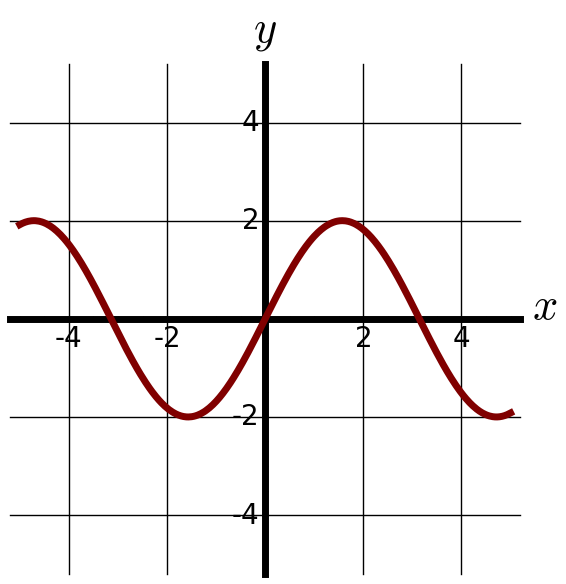
\includegraphics[width=0.2\textwidth]{img/chap1/sec1-2/prob3d.png} & 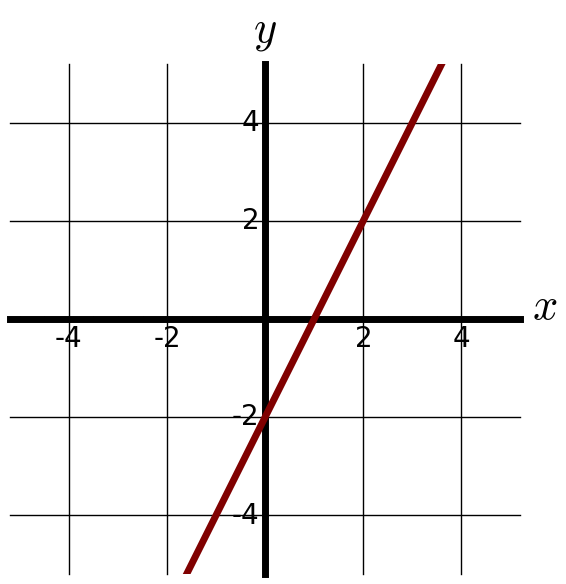
\includegraphics[width=0.2\textwidth]{img/chap1/sec1-2/prob3e.png} &
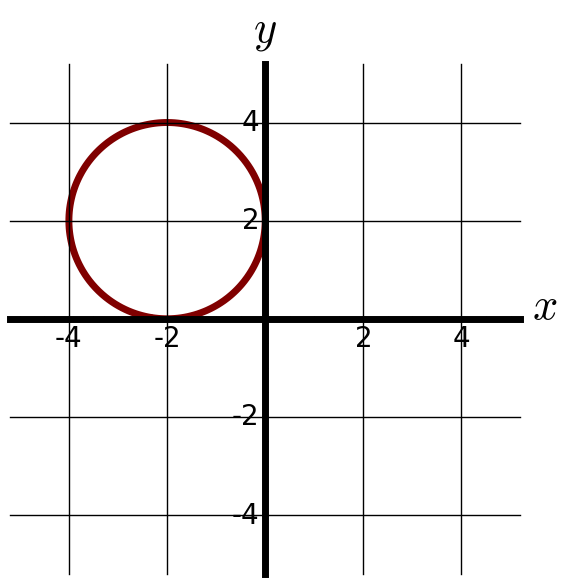
\includegraphics[width=0.2\textwidth]{img/chap1/sec1-2/prob3f.png} \\
\end{tabular}
\end{center}

\item  Select all of the following graphs which represent $y$ as a function of $x$.

\begin{center}
\begin{tabular}{ccc}
Graph A. & Graph B. & Graph C. \\
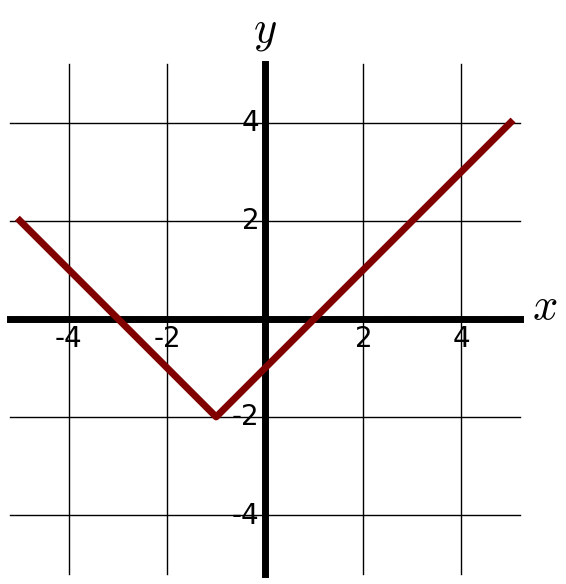
\includegraphics[width=0.2\textwidth]{img/chap1/sec1-2/prob4a.png} & 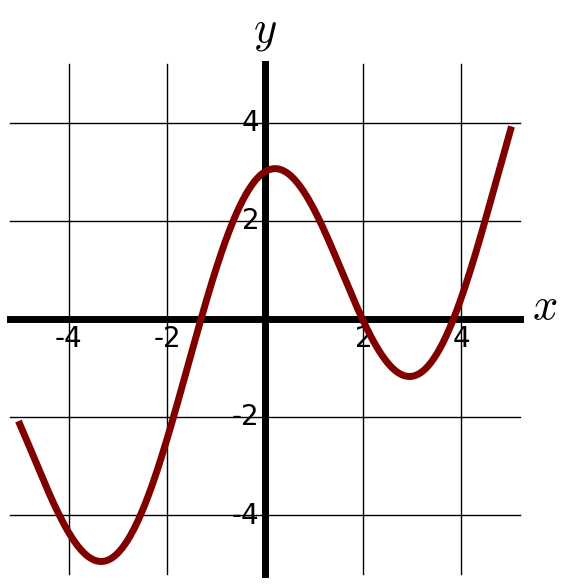
\includegraphics[width=0.2\textwidth]{img/chap1/sec1-2/prob4b.png} &
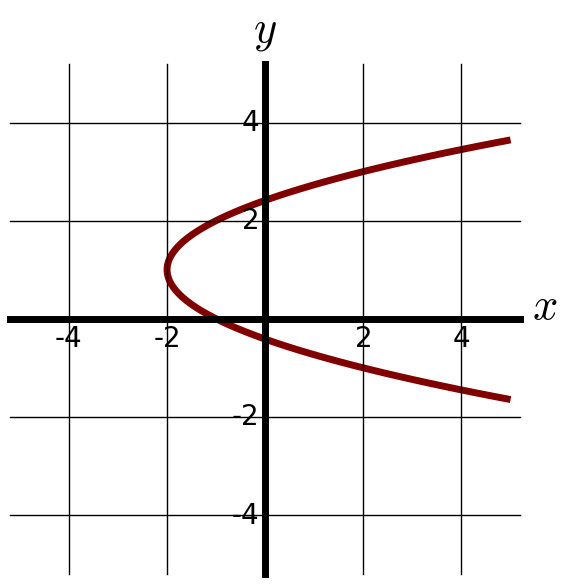
\includegraphics[width=0.2\textwidth]{img/chap1/sec1-2/prob4c.png} \\
\midrule
Graph D. & Graph E. & Graph F. \\
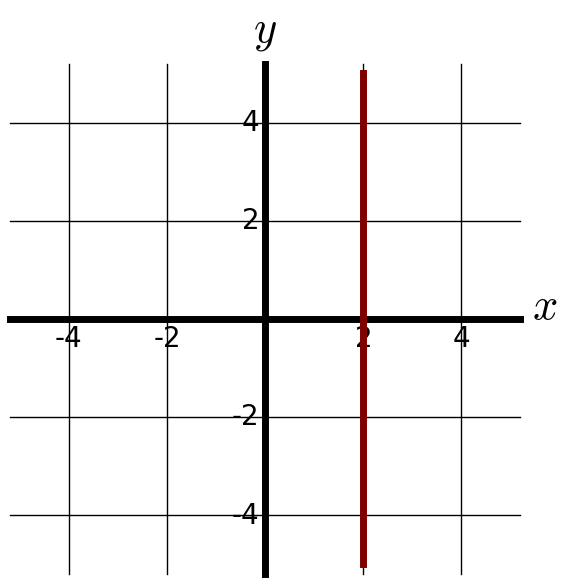
\includegraphics[width=0.2\textwidth]{img/chap1/sec1-2/prob4d.png} & 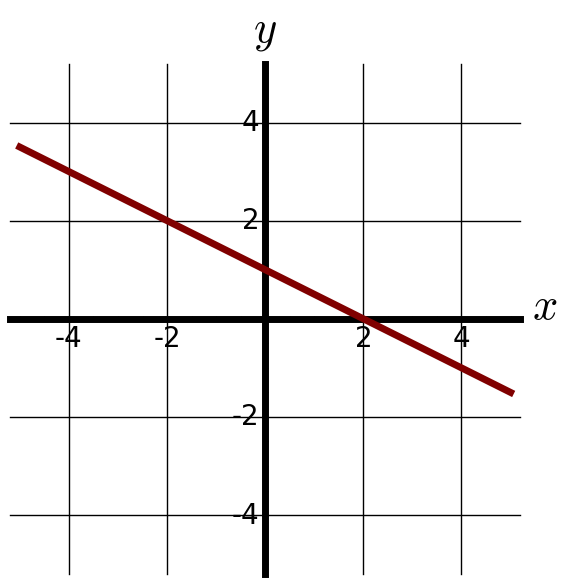
\includegraphics[width=0.2\textwidth]{img/chap1/sec1-2/prob4e.png} &
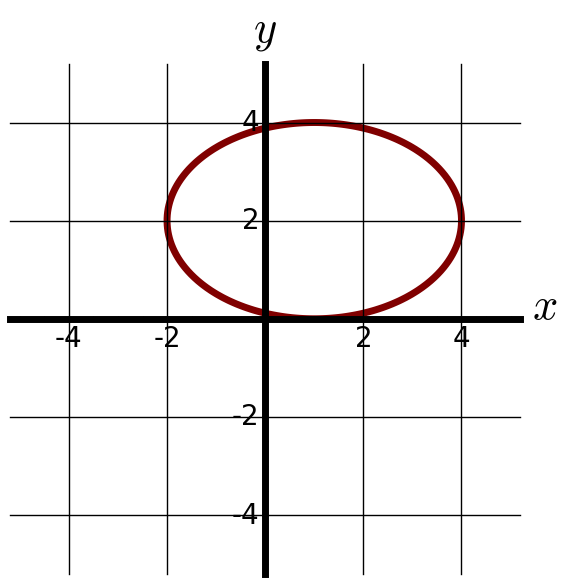
\includegraphics[width=0.2\textwidth]{img/chap1/sec1-2/prob4f.png} \\
\end{tabular}
\end{center}

\item Select all of the following tables which represent $y$ as a function of $x$.
\begin{center}
\begin{tabular}{ccc}
\begin{tabular}{rrrr}
\multicolumn{4}{c}{Table A.}\tabularnewline
\toprule
$x$ & 5 & 10 & 15\tabularnewline
\midrule
$y$ & 3 & 8 & 14\tabularnewline
\bottomrule
\end{tabular}
&
\begin{tabular}{rrrr}
\multicolumn{4}{c}{Table B.}\tabularnewline
\toprule
$x$ & 5 & 10 & 15\tabularnewline
\midrule
$y$ & 3 & 8 & 8\tabularnewline
\bottomrule
\end{tabular}
&
\begin{tabular}{rrrr}
\multicolumn{4}{c}{Table C.}\tabularnewline
\toprule
$x$ & 5 & 10 & 10\tabularnewline
\midrule
$y$ & 3 & 8 & 14\tabularnewline
\bottomrule
\end{tabular}
\end{tabular}
\end{center}

\item Select all of the following tables which represent $y$ as a function of $x$.
\begin{center}
\begin{tabular}{ccc}
\begin{tabular}{rrrr}
\multicolumn{4}{c}{Table A.}\tabularnewline
\toprule
$x$ & 2 & 6 & 13\tabularnewline
\midrule
$y$ & 3 & 10 & 10\tabularnewline
\bottomrule
\end{tabular}
&
\begin{tabular}{rrrr}
\multicolumn{4}{c}{Table B.}\tabularnewline
\toprule
$x$ & 2 & 6 & 6\tabularnewline
\midrule
$y$ & 3 & 10 & 14\tabularnewline
\bottomrule
\end{tabular}
&
\begin{tabular}{rrrr}
\multicolumn{4}{c}{Table C.}\tabularnewline
\toprule
$x$ & 2 & 6 & 13\tabularnewline
\midrule
$y$ & 3 & 10 & 14\tabularnewline
\bottomrule
\end{tabular}
\end{tabular}
\end{center}

\item Select all of the following tables which represent $y$ as a function of $x$.
\begin{center}
\begin{tabular}{cccc}
\begin{tabular}{rr}
\multicolumn{2}{c}{Table A.}\tabularnewline
\toprule
$x$ & $y$\tabularnewline
\midrule
0 & $-2$\tabularnewline
3 & 1\tabularnewline
4 & 6\tabularnewline
8 & 9\tabularnewline
3 & 1\tabularnewline
\bottomrule
\end{tabular}
&
\begin{tabular}{rr}
\multicolumn{2}{c}{Table B.}\tabularnewline
\toprule
$x$ & $y$\tabularnewline
\midrule
$-1$ & $-4$\tabularnewline
2 & 3\tabularnewline
5 & 4\tabularnewline
8 & 7\tabularnewline
12 & 11\tabularnewline
\bottomrule
\end{tabular}
&
\begin{tabular}{rr}
\multicolumn{2}{c}{Table C.}\tabularnewline
\toprule
$x$ & $y$\tabularnewline
\midrule
0 & $-5$\tabularnewline
3 & 1\tabularnewline
3 & 4\tabularnewline
9 & 8\tabularnewline
16 & 13\tabularnewline
\bottomrule
\end{tabular}
&
\begin{tabular}{rr}
\multicolumn{2}{c}{Table D.}\tabularnewline
\toprule
$x$ & $y$\tabularnewline
\midrule
$-1$ & $-4$\tabularnewline
1 & 2\tabularnewline
4 & 2\tabularnewline
9 & 7\tabularnewline
12 & 13\tabularnewline
\bottomrule
\end{tabular}
\end{tabular}
\end{center}

\item Select all of the following tables which represent $y$ as a function of $x$.

\begin{center}
\begin{tabular}{cccc}
\begin{tabular}{rr}
\multicolumn{2}{c}{Table A.}\tabularnewline
\toprule
$x$ & $y$\tabularnewline
\midrule
$-4$ & $-2$\tabularnewline
3 & 2\tabularnewline
6 & 4\tabularnewline
9 & 7\tabularnewline
12 & 16\tabularnewline
\bottomrule
\end{tabular}
&
\begin{tabular}{rr}
\multicolumn{2}{c}{Table B.}\tabularnewline
\toprule
$x$ & $y$\tabularnewline
\midrule
$-5$ & $-3$\tabularnewline
2 & 1\tabularnewline
2 & 4\tabularnewline
7 & 9\tabularnewline
11 & 10\tabularnewline
\bottomrule
\end{tabular}
&
\begin{tabular}{rr}
\multicolumn{2}{c}{Table C.}\tabularnewline
\toprule
$x$ & $y$\tabularnewline
\midrule
$-1$ & $-3$\tabularnewline
1 & 2\tabularnewline
5 & 4\tabularnewline
9 & 8\tabularnewline
1 & 2\tabularnewline
\bottomrule
\end{tabular}
&
\begin{tabular}{rr}
\multicolumn{2}{c}{Table D.}\tabularnewline
\toprule
$x$ & $y$\tabularnewline
\midrule
$-1$ & $-5$\tabularnewline
3 & 1\tabularnewline
5 & 1\tabularnewline
8 & 7\tabularnewline
14 & 12\tabularnewline
\bottomrule
\end{tabular}
\end{tabular}
\end{center}

\begin{minipage}{\linewidth}
\begin{wrapfigure}{r}{0.4\textwidth}
    \centering
    \vspace{-12pt}
    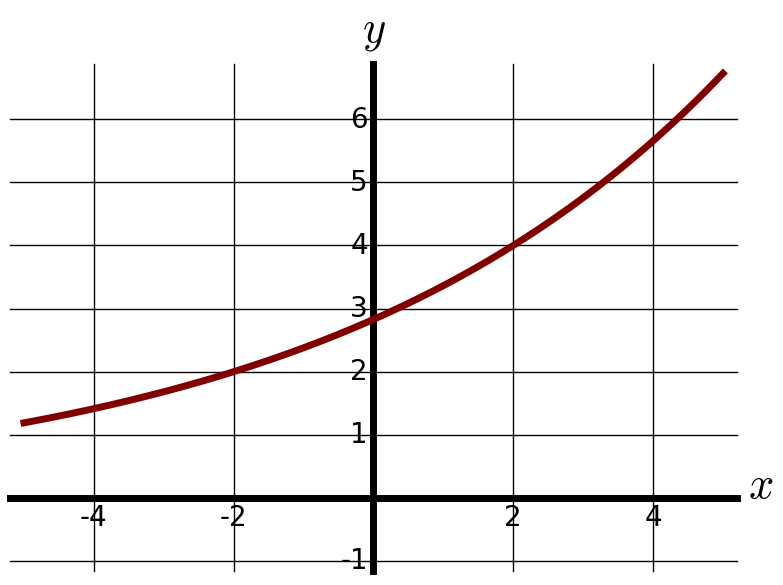
\includegraphics[width=0.4\textwidth]{img/chap1/sec1-2/prob7.png}
\end{wrapfigure}

\item Let $g(x)$ be the function graphed on the right.
    \begin{enumerate}
        \item Evaluate $g(2)$.
        \item Solve $g(x) = 2$ for $x$.
    \end{enumerate}
\end{minipage}

\vspace{120pt}

\begin{minipage}{\linewidth}
\begin{wrapfigure}{r}{0.4\textwidth}
    \centering
    \vspace{-36pt}
    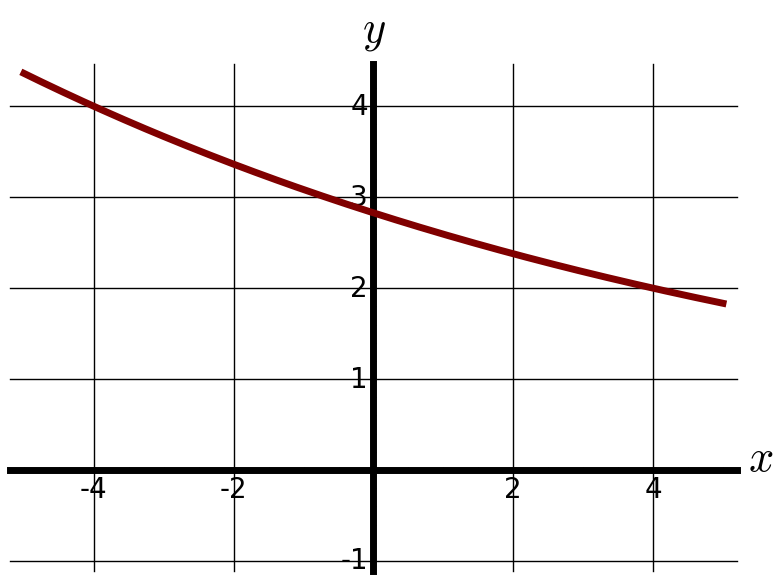
\includegraphics[width=0.4\textwidth]{img/chap1/sec1-2/prob8.png}
\end{wrapfigure}

\item Let $f(x)$ be the function graphed on the right.
    \begin{enumerate}
        \item Evaluate $f(4)$.
        \item Solve $f(x) = 4$ for $x$.
    \end{enumerate}
\end{minipage}


\vspace{120pt}

\begin{minipage}{\linewidth}
\begin{wraptable}{r}{0.6\textwidth}
    \centering
    \vspace{-12pt}
    \begin{longtable}[]{@{}lrrrrrrrrrr@{}}
    \toprule
    $x$ & 0 & 1 & 2 & 3 & 4 & 5 & 6 & 7 & 8 & 9\tabularnewline
    \midrule
    \endhead
    $f(x)$ & 74 & 28 & 1 & 53 & 56 & 3 & 36 & 45 & 14 & 47\tabularnewline
    \bottomrule
    \end{longtable}
\end{wraptable}

\item Consider the table at right.
    \begin{enumerate}
        \item Evaluate $f(3)$.
        \item Solve $f(x) = 1$ for $x$.
    \end{enumerate}
\end{minipage}

\begin{minipage}{\linewidth}
\begin{wraptable}{r}{0.6\textwidth}
    \centering
    \vspace{-12pt}
    \begin{longtable}[]{@{}lrrrrrrrrrr@{}}
    \toprule
    $x$ & 0 & 1 & 2 & 3 & 4 & 5 & 6 & 7 & 8 & 9\tabularnewline
    \midrule
    \endhead
    $g(x)$ & 62 & 8 & 7 & 38 & 86 & 73 & 70 & 39 & 75 & 34\tabularnewline
    \bottomrule
    \end{longtable}
\end{wraptable}

\item  Consider the table at right.
\begin{enumerate}
    \item Evaluate $g(8)$.
    \item Solve $g(x) = 7$ for $x$.
\end{enumerate}
\end{minipage}

\vspace{24pt}

\noindent For Exercises 15-22, evaluate: $f(-2)$, $f(-1)$, $f(0)$, $f(1)$, and $f(2)$, if possible.

\item $f(x) = 4 - 2 x$
\item $f(x) = 8-3x$
\item $f(x) = 8x^2 - 7x + 3$
\item $f(x) = 6x^2 - 7x + 4$
\item $f(x) = 3 + \sqrt{x+3}$
\item $f(x) = 4 - \sqrt[3]{x-2}$
\item $f(x) = \frac{x-3}{x+1}$
\item $f(x) = \frac{x-2}{x+2}$

\item Let $f(t) = 3t+5$.
\begin{enumerate}
    \item Evaluate $f(0)$.
    \item Solve $f(t) = 0$ for $t$.
\end{enumerate}

\item Let $g(p) = 6-2p$.
\begin{enumerate}
    \item Evaluate $g(0)$.
    \item Solve $g(p) = 0$ for $t$.
\end{enumerate}

\begin{minipage}{\linewidth}
\begin{wrapfigure}{r}{0.5\textwidth}
    \centering
    \vspace{-100pt}
    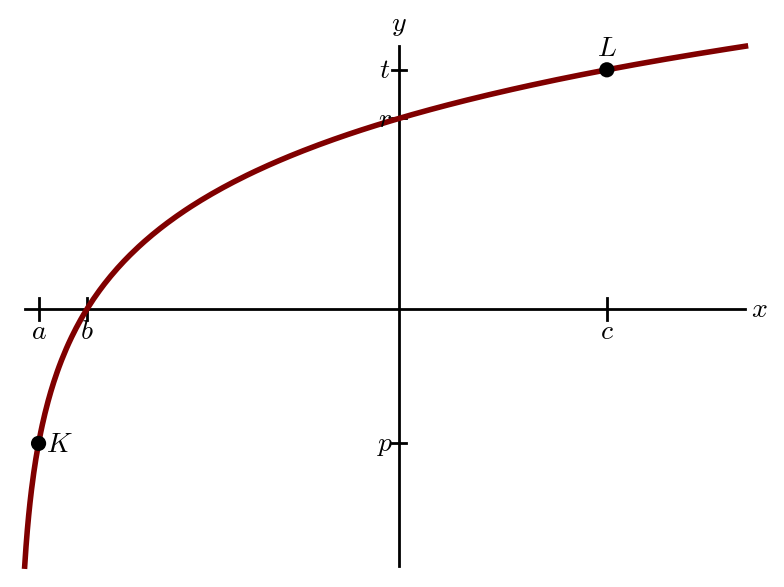
\includegraphics[width=0.48\textwidth]{img/chap1/sec1-2/prob21.png}
\end{wrapfigure}
\item Consider the graph of $f(x)$ on the right.
    \begin{enumerate}
        \item Evaluate $f(c)$.
        \item Solve $f(x) = p$ for $x$.
        \item Find the coordinates of points $L$ and $K$.
    \end{enumerate}
\end{minipage}
\end{enumerate}

\section{Models}
\label{sec:models}

\begin{center}
``All models are wrong; some models are useful." (George E.\ P.\ Box)
\end{center}

In the real world, we will, in all likelihood, have to work with data. ``Data-driven decisions" is a common phrase heard today. One thing that can be said is that real world data is messy and complex. Countless factors influence every phenomenon. Some factors are designed and some are purely random. Sometimes a data set is incomplete, missing pieces of data. Yet we may have to work with that data set as if it was complete. Sometimes we are tasked with {\bf forecasting}, which is predicting future data points, given the ones that we have.

\subsection{What is a Mathematical Model?}
\label{ssec:models}
In many different areas, we need tools to simplify a set of data and work with that simplified version of the data. These simplifications must be based on reasonable assumptions that connect to the larger context of the data. Simplifications serve two purposes. First, it may be impossible to take every variable into account. Second, models must often be communicated to others and a simple model is generally more clear and therefore much easier to communicate. This is the essence of what is called {\bf mathematical modeling}\index{Mathematical modeling}, or simply {\bf modeling}\index{Modeling}.

\begin{definition}
A {\bf model} \index{model} or a {\bf mathematical model} is a mathematical framework to help describe some phenomenon, specifically how an input or quantity affects or relates to some output.  A model has three main components:
\begin{enumerate}
    \item One or more input variables, with specific descriptions of what these variables represent, including units.
    \item One or more functions, with specific descriptions of what the output of the functions represent, including units.
    \item A domain and/or range over which the function(s) make sense to use.
\end{enumerate}
Additionally, we may want to consider the following when creating a model.
\begin{itemize}
    \item Identify underlying assumptions that were used to simplify the situation.
    \item Perform a sensitivity analysis to determine if the model is relatively unchanged if the data varies slightly.
\end{itemize}
\end{definition}

For example, one could construct a model to speculate how the price of an item affects the demand for that item, and from that, predict revenue from sales of that item.

It is crucial to state that a model is used to simplify reality and does not dictate or reflect past, present, or future reality with absolute precision. Although good models can be useful for forecasting, decision-making, and filling in missing data. That is the essence of the quote at the beginning of the section by the late George Box, a famous British statistician.

%\begin{wrapfigure}{R}{0.3\textwidth}
\begin{floatingfigure}{0.3\textwidth}
    \centering
    %\vspace{-20pt}
    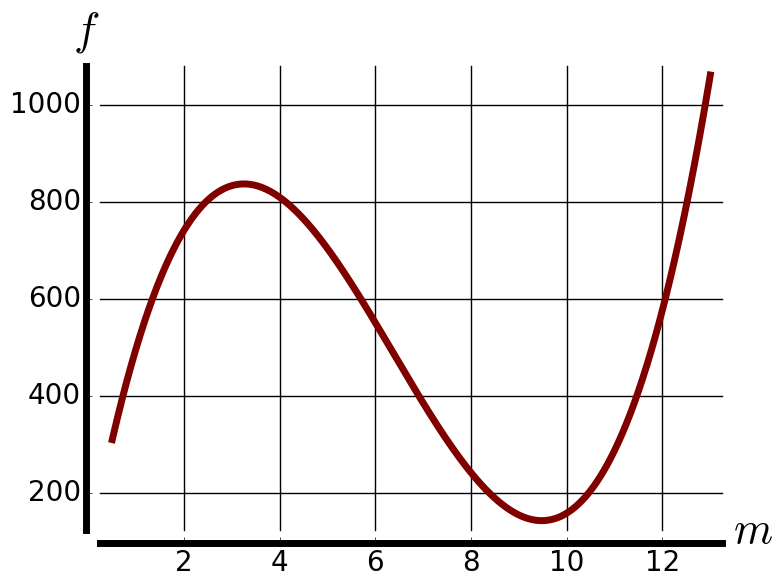
\includegraphics[width=0.3\textwidth]{img/chap1/sec1-3/fig1-3-oil.png}\\
    \caption{Fuel Oil Usage by Plant W in 2016.}
    \label{fig:1-3-oil-curve}
    %\vspace{-12pt}
\end{floatingfigure}
%\end{wrapfigure}

The following is an example of a mathematical model, based on an actual data set from ``Plant W." We will analyze this scenario in several places in this text and.

{\bf Model:} Plant W heats an external tank and powers their operations by burning fuel oil. The rate at which they burned this oil in 2016 can be described by the following model. Let $m$ be the month of the year, with 1 referring to January 1, and 12 referring to December 1, so that $1\le m < 13$. Let $f(m)$ describe the rate at which the fuel burns, in gallons per month. A model for $f(m)$ is
$$f(m) = 5.76m^3 - 109.98m^2 + 532.58m + 70.17\mbox{ gallons per month.}$$
Figure \ref{fig:1-3-oil-curve} plots this curve over the given domain.

{\bf Commentary:} Note that in this example, we clearly described the input variable, what it represented, a domain that it makes sense over, and gave the units (months). We clearly described the function (the output), what it modeled, and gave the units.

Examining the graph of the function, we can see that the model makes sense, based on the context. If Plant W is heating a large external tank, then in the winter and early spring, we expect more oil to be used to heat it. This tank may also have retained some heat, as fluids tend to do, from the late summer and fall. We expect a significant drop in oil usage through the late spring and summer months and finally a significant increase in oil usage during the fall and early winter.

Is the model precise? Of course not. First, we know that in 2016 (a leap year), there were months with 29, 30, or 31 days, yet we treated each month as equal. Perhaps a better model would have modeled fuel usage per day. For the sake of clarity, however, we aggregated the days into months; we know immediately that month 6 is June, but do not immediately know which month is day 276, for example.

A second reason that we know that the model is not accurate is that we can't be certain that on January 1, 2016 that Plant W burned oil at a rate of $f(1) = 498.53$ gallons per month. In other words, on January 1, 2016, did Plant W burn $f(1)/31 = 16.08$ gallons of fuel oil? We can be almost certain that they did not, but the actual amount may have been somewhat close to that. Other factors that we didn't consider were the range of temperatures that day and the percentage of the tank that was full. Considering these factors would make the model more accurate, but more complex.

A third item to consider is that in this case, we are dealing with a yearly cycle. We should expect $f(1)$ to be really close to $f(13)$, since both input values would refer to January 1 in 2016 and 2017, respectively. However, we have
$$ f(1) = 498.53 \quad \mbox{and} \quad f(13) = 1061.81 \enspace ,$$
which is a significant difference. Perhaps a better model would attempt to get these two points either closer to each other or make them exactly equal to each other. Section \ref{sec:trig} will describe how to work with periodic or seasonal data such as this. \hfill$\blacksquare$

\subsection{Curve Fitting, Interpolation, and Extrapolation}
\label{ssec:cfie}

%\begin{wrapfigure}{R}{0.3\textwidth}
\begin{floatingfigure}{0.3\textwidth}
    \centering
    %\vspace{-20pt}
    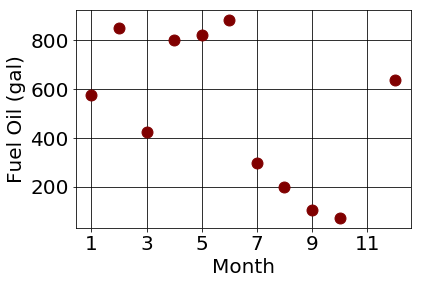
\includegraphics[width=0.3\textwidth]{img/chap1/sec1-3/ex1-3-oil.png}\\
    \caption{Fuel Oil Usage by Plant W in 2016.}
    \label{fig:1-3-oil}
    %\vspace{-20pt}
\end{floatingfigure}
%\end{wrapfigure}
A common way to create a mathematical model is to create a {\bf scatter plot}\index{Scatter plot} of a data set and determine a graph that is a reasonable fit to the curve, given the scenario. Figure \ref{fig:1-3-oil} gives an example of a scatter plot of data from Table \ref{tab:1-3-oil} that will be used in Example \ref{ex:interpolation}. A scatter plot is simply a representation of data in which each element of a data set can be represented as a point on a set of coordinate axes.

{\bf Curve fitting}\index{Curve fitting} is a technique in which one creates a continuous function to smooth out discrete data. The curve will generally not ``connect the dots" of a scatter plot of the data, but will give the general behavior of the data. The most common and well-known means to fit a curve to data is by creating a {\bf regression curve}\index{Curve!regression}\index{Regression} of the data. The mathematical details of how to make these curves is outside the scope of this text. It is sufficient to understand that regression curves are {\bf curves of best fit}\index{Curve!best fit} or {\bf best fit curves}.

% Future feature: show how to use Excel and/or Python.

With an appropriate curve fit to data, we can {\bf interpolate}\index{Interpolation} and {\bf extrapolate}\index{Extrapolation} the data.

\begin{definition}
Using the graph of a function to estimate values between known data points (i.e., within the domain) is called {\bf interpolation}. Making predictions beyond the domain of known data is called {\bf extrapolation}.
\end{definition}

\paragraph{Interpolation.} In cases in which there is missing data, we can use interpolation techniques to make educated guesses for the actual data. This is just one example in which interpolation is used. The following example uses regression curves and another simpler technique.

\begin{example}
\label{ex:interpolation}
Plant W, mentioned earlier, powers their operations by burning fuel oil. Table \ref{tab:1-3-oil} below shows how much oil they burned in 2016, but they are missing data from November. (Figure \ref{fig:1-3-oil} gave a scatter plot of this data.) What are some reasonable values for the amount of fuel oil that they burned in November 2016?

\begin{table}[h!]
\centering
\begin{tabular}{l*{12}{c}}
\toprule
Month & Jan. & Feb. & Mar. & Apr. & May & June & July & Aug. & Sep. & Oct. & Nov. & Dec. \\
\midrule
Oil (gal) & 573.0 & 850.0 &  425.3 & 800.1  & 818.9 &  880.9 &  296.5 & 198.7 & 105.4 & 72.0 & ?? & 638.0\\
\bottomrule
\end{tabular}
\caption{Fuel Oil Usage at Plant W in 2016}
\label{tab:1-3-oil}
\end{table}
\solution We will show two ways to estimate the missing data point. The first is straightforward. The other will use a model developed from a regression curve, applying concepts and techniques that we will learn more about in Section \ref{sec:polynomial}.

A simple way to interpolate a missing data point is to find the average (or mean) of the data point before and the data point after the missing point. With this approach, we have an estimate for the November 2016 fuel oil consumption of
$$\frac{72.0 + 638.0}{2} \mbox{ gallons} = \frac{710.0}{2} \mbox{ gallons} = 355 \mbox{ gallons.}$$

\begin{floatingfigure}{0.3\textwidth}
    \centering
    %\vspace{-20pt}
    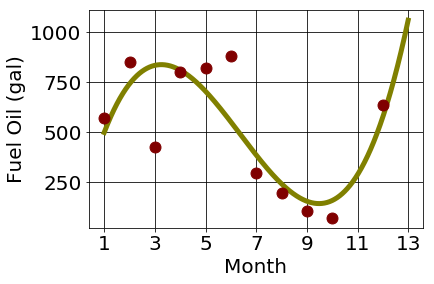
\includegraphics[width=0.3\textwidth]{img/chap1/sec1-3/fig1-3-oil-curve.png}\\
    \caption{Model of Fuel Oil Usage by Plant W in 2016.}
    \label{fig:1-3-oil-model}
    %\vspace{-20pt}
\end{floatingfigure}
The second method creates a model by finding a curve the best fits the data in Table \ref{tab:1-3-oil}. The volume of fuel oil burned by Plant W in month $m$ of 2016 is
$$f(m) = 5.76m^3 - 109.98m^2 + 532.58m + 70.17\mbox{ gallons.}$$
This model is plotted with the data in Figure \ref{fig:1-3-oil-model}, showing that the model is reasonable.

From this model, we can estimate that Plant W burned
$$f(11) = 5.76\cdot 11^3 - 109.98\cdot 11^2 + 532.58\cdot 11 + 70.17\mbox{ gallons} = 287.53 \mbox{ gallons}$$
in November (month $m=11$).
\end{example}

\paragraph{Extrapolation.} In contrast to interpolation, extrapolation is more difficult because it involves predicting data points beyond the domain of the data using the trends that currently exist. Extra care must be used to create and justify assumptions used to develop the model that is used to extrapolate.

Let's discuss the following table and plot of winning Men's and Women's 100 meter dash times in the Olympics. As of this writing, the next summer Olympics will be in 2020, so we can extrapolate from the given data to predict the winning times in the next Olympics. When we plot the data, however, many more questions will naturally arise and the answers to those questions will vary depending on the model that we use to describe the data.

\begin{table}[h!]
\centering
\begin{tabular}{l*{11}{r}}
\toprule
Year        & 1928 & 1932 & 1936 & 1948 & 1952 & 1956 & 1960 & 1964 & 1968 & 1972  & 1976 \\
\midrule
Time (M, s) & 10.8 & 10.3 & 10.3 & 10.3 & 10.4 & 10.5 & 10.2 & 10.0 & 9.95 & 10.14 & 10.06 \\
\midrule
Time (W, s) & 12.2 & 11.9 & 11.5 & 11.9 & 11.5 & 11.5 & 11.0 & 11.4 & 11.0 & 11.07 & 11.08 \\
\bottomrule
Year        &  1980 & 1984 & 1988 & 1992 & 1996 & 2000 & 2004 & 2008 & 2012 & 2016 & 2020 \\
\midrule
Time (M, s) & 10.25 & 9.99 & 9.92 & 9.96 & 9.84 & 9.87 & 9.85 & 9.69 & 9.63 & 9.81 & ???? \\
\midrule
Time (W, s) & 11.06 & 10.97 & 10.54 & 10.82 & 10.94 & 11.12 & 10.93 & 10.78 & 10.75 & 10.71 & ???? \\
\bottomrule
\end{tabular}
\caption{Winning Men's and Women's 100 Meter Dash Times in the Olympics}
\label{tab:1-3-dash}
\end{table}

\begin{floatingfigure}{0.4\textwidth}
%\begin{figure}[ht!]
    \centering
    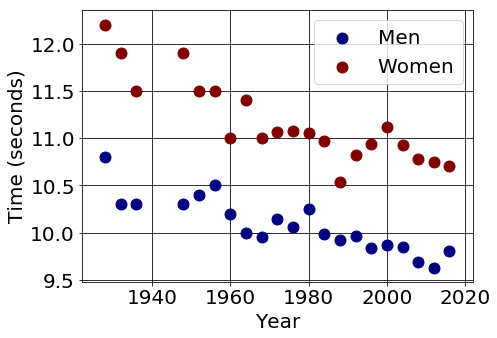
\includegraphics[width=0.4\textwidth]{img/chap1/sec1-3/fig1-3-dash.png}\\
    \caption{Winning Olympic 100-Meter Dash Times}
    \label{fig:1-3-dash}
    \vspace{-20pt}
\end{floatingfigure}
%\end{figure}
Figure \ref{fig:1-3-dash} gives a scatter plot of the data. It's clear that there has been a downward trend in the gold medal times over the past century, but it's not a smooth trend. The data is choppy. The simplest curve-fitting model to smooth out the data is to use a best fit line. In the next section, we will learn how to find best fit lines, but for now, we will describe the model and discuss the model.

{\bf Model: } Let $y$ be the year and $1928\le y\le 2016$. Then the winning men's and women's 100-meter dash times in the Olympics in year $y$ can be described by $m(y)$ and $w(y)$, respectively.
\begin{align}
\label{eq:1-3-dash}
m(y) &= -0.009498y + 28.841\mbox{ seconds}\\
w(y) &= -0.014185y + 39.188 \mbox{ seconds}\nonumber
\end{align}

\begin{floatingfigure}{0.4\textwidth}
%\begin{figure}[ht!]
    \centering
    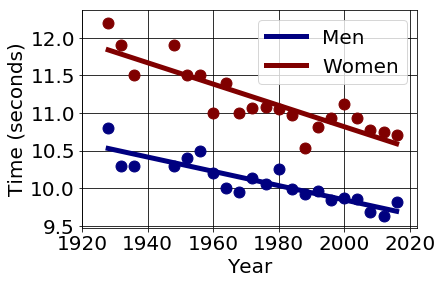
\includegraphics[width=0.4\textwidth]{img/chap1/sec1-3/fig1-3-dash-curve.png}\\
    \caption{Winning Olympic 100-Meter Dash Times with Models}
    \label{fig:1-3-dash-curve}
    \vspace{12pt}
\end{floatingfigure}
%\end{figure}
Note that we have all the necessary components of a model: (1) a description of the input variable ($y$), with the units (years), (2) a description of the functions ($m$ and $w$) and their units (seconds), and (3) a domain over which the models make sense. A plot of the models with the scatter plot of the data shows that the models make sense.

\begin{example}
Given the data in Table \ref{tab:1-3-dash} and the models in \eqref{eq:1-3-dash}, what are reasonable predictions for the winning times in the 100-meter dash at the 2020 Olympics?

\begin{solution}
Since $y$ is the year of the Olympics, then we predict the winning time for the men's 100-meter dash to be
$$m(2020) = -0.009498\cdot 2020 + 28.841\mbox{ seconds} = 9.66 \mbox{ seconds}$$
and for the women's 100-dash:
$$w(2020) = -0.014185\cdot 2020 + 39.188\mbox{ seconds} = 10.53 \mbox{ seconds.}$$

These times aren't completely unreasonable, given the data, but taken in context, one might be a bit skeptical of these predictions. For the men's 100-meter dash, the time of 9.66 would be only 0.03 slower than the Olympic record, held by Usain Bolt of Jamaica. Bolt ran the three fastest Olympic 100-meter dashes at the 2008, 2012, and 2016 Olympics, but has since retired from sprinting. The forecast women's time would beat Florence Griffith-Joyner's world record, set in 1988, by 0.01 second.
\end{solution}
\end{example}

To create a better model, we could include data from other races, not just the Olympics. We could also consider curves other than lines. To see why extrapolation has it's limitations with the linear model, consider the predicted winning times for the Olympics in the year 3000. For the men:
$$m(3000) = -0.009498\cdot 3000 + 28.841\mbox{ seconds} = 0.347 \mbox{ seconds}$$
and for the women's 100-meter dash:
$$w(3000) = -0.014185\cdot 3000 + 39.188\mbox{ seconds} = -3.37 \mbox{ seconds.}$$
These times are clearly absurd. The men's time would require a runner to run faster than a race car and for the women, no one can run a race in negative time. Therefore, the further out we attempt to extrapolate, the less plausible and more uncertain the results are.

The plot also gives us a question to consider. Notice that the women's times are decreasing more rapidly than the men's times. Will a woman ever run the 100 meter dash faster than a man in a single Olympics? The model predicts that this could happen, but the winning times would again be absurd.



% Curve-Fitting: testing/training.

\section{Linear Functions}
\label{sec:linear}

\section{Polynomial Functions}
\label{sec:polynomial}

\section{Exponential Functions}
\label{sec:exp}

\subsection{Laws of Exponents}
\label{ssec:laws-exp}

The Laws of Exponents let you rewrite algebraic expressions that involve exponents. The last three listed here are really definitions rather than rules.

\begin{theorem}[Laws of Exponents\index{Laws of Exponents}]
All variables here represent real numbers and all variables in denominators are nonzero.
\begin{enumerate}
    \item $x^a\cdot x^b=x^{a+b}$
		\item $\dfrac{x^a}{x^b}=x^{a-b}$
		\item $\left(x^a\right)^b=x^{ab}$
		\item $(xy)^a=x^a y^a$
		\item $\left(\dfrac{x}{y}\right)^b=\dfrac{x^b}{y^b}$
		\item $x^0=1$, provided $x\neq 0$, although in some contexts, $0^0 = 1$.
		\item $x^{-n}=\dfrac{1}{x^n}$, provided $x\neq 0$.
		\item $x^{1/n}=\sqrt[n]{x}$, provided $x\neq 0$.
\end{enumerate}
\end{theorem}

\begin{example}
Simplify $\left(2x^2\right)^3(4x)$.

\solution We'll begin by simplifying the $\left(2x^2\right)^3$ portion. Using Property 4, we can write
\begin{align*}
\left(2x^2\right)^3 &= 2^3\left(x^2\right)^3(4x)& &\mbox{Use Property 4.}\\
  &= 8x^6(4x)&                  &\mbox{Evaluate $2^3=8$, and use Property 3.}	\\
  &= 32x^7&                     &\mbox{Multiply the constants, and use Property 1, recalling $x=x^1$.}
\end{align*}
\end{example}

Being able to work with negative and fractional exponents will be very important later in this course.

\begin{example}
Rewrite \(\dfrac{5}{x^3}\) using negative exponents.

\solution Since \(x^{-n}=\dfrac{1}{x^n}\), then \(x^{-3}=\dfrac{1}{x^3}\) and thus
\[\dfrac{5}{x^3}=5x^{-3}.\]
\end{example}

\begin{example}
Simplify \(\left(\dfrac{x^{-2}}{y^{-3}}\right)^2\) as much as possible and write your answer using only positive exponents.

\solution
\begin{align*}
		\left(\dfrac{x^{-2}}{y^{-3}}\right)^2 &=  \dfrac{\left(x^{-2}\right)^2}{\left(y^{-3}\right)^2}\\
		 &=  \dfrac{x^{-4}}{y^{-6}}\\
		 &=  \dfrac{y^6}{x^4}
	\end{align*}
\end{example}

\begin{example}
Rewrite \( \left(\sqrt{p^5}\right)^{-1/3} \) using exponents.

\solution A square root is a radical with index of two. In other words, \(\sqrt{x}=\sqrt[2]{x}\). Using the exponent rule above, \(\sqrt{x}=\sqrt[2]{x}=x^{1/2}\). Rewriting the square roots using the fractional exponent, \[4\sqrt{x}-\dfrac{3}{\sqrt{x}}=4x^{1/2}-\dfrac{3}{x^{1/2}}.\]

Now we can use the negative exponent rule to rewrite the second term in the expression:
\[4x^{1/2}-\dfrac{3}{x^{1/2}}=4x^{1/2}-3x^{-1/2}.\]
\end{example}

\begin{example}
Rewrite \( \left(\sqrt{p^5}\right)^{-1/3} \) using only positive exponents.

\solution
  \begin{align*}
		\left(\sqrt{p^5}\right)^{-1/3} &=  \left(\left(p^5\right)^{1/2}\right)^{-1/3}\\
		 &=  p^{-5/6}\\
		 &=  \frac{1}{ p^{5/6}}
	\end{align*}
\end{example}

\begin{example}
Rewrite \( x^{-4/3} \) as a radical.

\solution
\begin{align*}
		x^{-4/3} &=  \frac{1}{x^{4/3}} \\
		 &=  \frac{1}{\left(x^{1/3}\right)^4} \quad \text{(since \(\frac{4}{3}=4\cdot\frac{1}{3}\))}\\
		 &=  \frac{1}{\left(\sqrt[3]{x}\right)^4} \quad \text{(using the radical equivalence)}
	\end{align*}
\end{example}

\subsection{Exponential Models}
\label{ssec:models-exp}

Consider these two companies:
\begin{itemize}
  \item Company A has 100 stores, and expands by opening 50 new stores a year
  \item Company B has 100 stores, and expands by increasing the number of stores by 50\% of their total each year.
\end{itemize}
Company A is exhibiting linear growth. In linear growth, we have a constant rate of change -- a constant number that the output increased for each increase in input. For company A, the number of new stores per year is the same each year.

Company B is different -- we have a percent rate of change rather than a constant number of stores/year as our rate of change. To see the significance of this difference compare a 50\% increase when there are 100 stores to a 50\% increase when there are 1000 stores:
\begin{itemize}
  \item 100 stores, a 50\% increase is 50 stores in that year.
  \item 1000 stores, a 50\% increase is 500 stores in that year.
\end{itemize}
Calculating the number of stores after several years, we can clearly see the difference in results.

\begin{table}[!ht]
  \centering
  \begin{tabular}{rrr}
    \toprule
    Years	& Company A	& Company B	\\
    \midrule
    2	 & 200 & 	225	\\
    4	& 300	& 506	\\
    6	& 400	& 1139	\\
    8	& 500 &	2563	\\
    10&	600 & 	5767\\
    \bottomrule
  \end{tabular}
\end{table}

\begin{figure}[!ht]
\centering
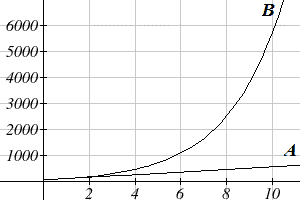
\includegraphics[width=0.5\textwidth]{img/chap1/sec1-6/image072.png}
\caption{Graphs of data from A and B, with B fit to a curve.}
\end{figure}

This percent growth can be modeled with an {\bf exponential function}\index{Function!exponential}.

\begin{definition}[Exponential Function]
An {\bf exponential growth}\index{Exponential growth} or {\bf decay}\index{Exponential decay} function is a function that grows or shrinks at a constant percent growth rate. The equation can be written in the form
$$f(x) = a\cdot(1+r)^x$$
or
$$f(x)=a\cdot b^x \enspace ,$$
where
\begin{itemize}
  \item[$a$] is the {\bf initial or starting value}\index{Initial value}\index{Starting value} of the function,
  \item[$r$] is the {\bf percent growth or decay rate}\index{Rate!decay}\index{Rate!growth}, written as a decimal,
  \item[$b$] is the {\bf growth factor}\index{Growth factor} or {\bf growth multiplier}\index{Growth multiplier}: $b=1+r$.
\end{itemize}
Since powers of negative numbers behave strangely, we must have $b>0$.
\end{definition}

\begin{example}
India's population was 1.14 billion in the year 2008 and is growing by about 1.34\% each year. Write an exponential function for India's population, and use it to predict the population in 2020.

\solution Using 2008 as our starting time ($t=0$), our initial population will be 1.14 billion. Since the percent growth rate was 1.34\%, our value for $r$ is 0.0134.

Using the basic formula for exponential growth $f(x)=a(1+r)^xx$, we can write the formula,
$$f(t)=1.14(1+0.0134)^t$$
To estimate the population in 2020, we evaluate the function at $t=12$, since 2020 is 12 years after 2008:
$$f(t)=1.14(1+0.0134)^{12}\approx1.337 \mbox{ billion people in 2020.}$$
\end{example}

\begin{example}
A certificate of deposit (CD) is a type of savings account offered by banks, typically offering a higher interest rate in return for a fixed length of time you will leave your money invested. If a bank offers a 24 month CD with an annual interest rate of 1.2\% compounded monthly, how much will a \$1000 investment grow to over those 24 months? What is the equivalent annual percentage yield (APY)?

\solution First, we must notice that the interest rate is an annual rate, but is compounded monthly, meaning interest is calculated and added to the account monthly. To find the monthly interest rate, we divide the annual rate of 1.2\% by 12 since there are 12 months in a year: $\frac{1.2\%}{12} = 0.1\%$. Each month we will earn 0.1\% interest. From this, we can set up an exponential function, with our initial amount of \$1000 and a growth rate of $r=0.001$, and our input $m$ measured in months:
$$f(m)=1000\left(1+\frac{0.012}{12}\right)^m=1000(1.001)^m \enspace .$$
After 24 months, the account will have grown to $f(24)=1000(1.001)^{24}\approx\$1024.28.$

The annual percentage yield (APY) is the interest rate that is equivalent to 1.2\% compounded quarterly if we were to compound annually instead. So we will calculate how much our investment grows in one year (expressed as a percentage of the original amount), which means using $m=12$ months:
$$f(12)=1000(1.001)^{12}\approx\$1012.07 \enspace ,$$
so we have
$$\frac{\mbox{Final value}}{\mbox{Initial value}} = \frac{\$1012.07}{\$1000}=1.01207$$
or $101.207\%$ of what we started with, which is a 1.207\% gain. Thus our APY is 1.207\%. This answer seems reasonable since when compounding quarterly we earn interest on interest from the previous quarters, so to compensate for the fact that we are not compounding as often we need a slightly higher rate to earn an equal amount.
\end{example}

\begin{example}
Bismuth-210 is an isotope that radioactively decays by about 13\% each day, meaning 13\% of the remaining Bismuth-210 transforms into another atom (Polonium-210 in this case) each day. If you begin with 100 mg of Bismuth-210, how much remains after one week?

\solution With radioactive decay, instead of the quantity increasing at a percent rate, the quantity is decreasing at a percent rate. Our initial quantity is $a=100$ mg, and our growth rate will be negative 13\%, since we are decreasing: $r=-0.13$. This gives the equation
$$Q(d)=100(1-0.13)^d=100(0.87)^d \enspace .$$
This can also be explained by recognizing that if 13\% decays, then 87 \% remains.

After one week, 7 days, the quantity remaining would be $Q(7)=100(0.87)^7=37.73$ mg of Bismuth-210.
\end{example}

\begin{example}
$T(q)$ represents the total number of Android smart phone contracts, in thousands, held by a certain Verizon store region measured quarterly since January 1, 2010. Interpret all of the parts of the equation $T(2)=86(1.64)^2=231.3056$ .

\solution Interpreting this from the basic exponential form, we know that 86 is our initial value. This means that on Jan. 1, 2010 this region had 86,000 Android smart phone contracts. Since $b=1+r=1.64$, we know that every quarter the number of smart phone contracts grows by 64\%. $T(2)=231.3056$ means that in the second quarter (or at the end of the second quarter) there were approximately 231,305 Android smart phone contracts.
\end{example}

When working with exponentials, there is a special constant we must talk about. It arises when we talk about things growing continuously, such as continuous compounding, or natural phenomena like radioactive decay that happen continuously.

\begin{definition}[Euler's Number: $e$]
$$e\approx2.718282$$
\end{definition}
Because $e$ is often used as the base of an exponential, most scientific and graphing calculators have a button that can calculate powers of $e$, usually labeled $e^x$. Some computer software instead defines a function $\exp(x)$, where $\exp(x) = e^x$. Since calculus studies continuous change, we will almost always use the $e$-based form of exponential equations in this course.

\begin{definition}[Continuous Growth Formula]
{\bf Continuous growth}\index{Continuous growth} can be calculated using the formula
$$f(x)=a\cdot e^{rx} \enspace ,$$
where
\begin{itemize}
    \item[$a$] is the {\bf starting amount}\index{Initial value}\index{Starting value} or {\bf initial quantity},
    \item[$r$] is the {\bf continuous growth rate}\index{Growth rate}.
\end{itemize}
\end{definition}

\begin{example}
Radon-222 decays at a continuous rate of 17.3\% per day. How much will 100mg of Radon-222 decay to in 3 days?

\solution Since we are given a continuous decay rate, we use the continuous growth formula. Since the substance is decaying, we know the growth rate will be negative: $r=-0.173$, $f(3)=100e^{-0.173\cdot 3}\approx 59.512$ mg of Radon-222 will remain.
\end{example}

\subsection{Graphs of Exponential Functions}
\label{ssec:graphs-exp}

\begin{theorem}[Graphical Features of Exponential Functions]
In the graph of the function $f(x) = a\cdot b^x$, we have the following.

\begin{itemize}
  \item $a$ is the {\bf vertical intercept} of the graph.
  \item $b$ determines the {\bf rate} at which the graph grows:
  \begin{itemize}
      \item the function will {\bf increase} if $b>1$,
      \item the function will {\bf decrease} if $0<b<1$.
  \end{itemize}
  \item The graph will have a {\bf horizontal asymptote} at $y=0$.
  \item The graph will be:
  \begin{itemize}
    \item {\bf concave up} if $a>0$
    \item {\bf concave down} if $a<0$.
  \end{itemize}
  \item The {\bf domain} of the function is all real numbers, $\R$.
  \item The {\bf range} of the function is $(0,\infty)$ if $a>0$, and $(-\infty,0)$ if $a<0$.
\end{itemize}
\end{theorem}

When sketching the graph of an exponential function, it can be helpful to remember that the graph will pass through the points $(0,a)$ and $(1, ab)$.

\begin{theorem}
The value $b$ will determine the function's long run behavior. The notation $x\to\infty$ means ``as the value of $x$ grows (without bound) to infinity ($\infty$)," or, more briefly, ``as $x$ goes to $\infty$."
\begin{itemize}
  \item If $b>1$:
  \begin{itemize}
    \item As $x\rightarrow\infty$, $f(x)\rightarrow\infty$.
    \item As $x\rightarrow-\infty$, $f(x)\rightarrow 0$.
  \end{itemize}
  \item If $0<b<1$:
  \begin{itemize}
    \item As $x\rightarrow\infty$, $f(x)\rightarrow 0$.
    \item As $x\rightarrow-\infty$, $f(x)\rightarrow\infty$.
  \end{itemize}
\end{itemize}
\end{theorem}

\begin{example}
Sketch a graph of $f(x) = 4\cdot \left(\frac{1}{3}\right)^x$.

\solution This graph will have a vertical intercept at the point $(0,4)$, and passes through the point $\left(1,\frac{4}{3}\right)$. Since $b<1$, the graph will be decreasing towards zero. Since $a>0$, the graph will be concave up.

\begin{figure}[!ht]
\centering
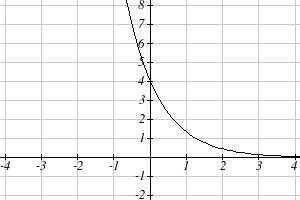
\includegraphics[width=0.5\textwidth]{img/chap1/sec1-6/image073.png}
\caption{}
\end{figure}
We can also see from the graph the long run behavior: as $x\rightarrow\infty$, $f(x)\rightarrow 0$, and as $x\rightarrow-\infty$, $f(x)\rightarrow\infty$.
\end{example}

To get a better feeling for the effect of the coefficients $a$ and $b$ on the graph, examine the sets of graphs below. The first set shows various graphs, where $a$ remains the same and we only change the value for $b$. Notice that the closer the value of $b$ is to 1, the less steep the graph will be.

\begin{figure}[!ht]
\centering
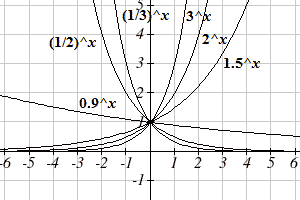
\includegraphics[width=0.5\textwidth]{img/chap1/sec1-6/image074.png}
\caption{Changing the value of $b$.}
\end{figure}

In the next set of graphs, $a$ is altered and our value for $b$ remains the same.

\begin{figure}[!ht]
\centering
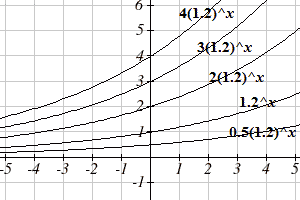
\includegraphics[width=0.5\textwidth]{img/chap1/sec1-6/image075.png}
\caption{Changing the value of $a$.}
\end{figure}

Notice that changing the value for $a$ changes the vertical intercept. Since $a$ is multiplying the $b^x$ term, $a$ acts as a vertical stretch factor, not as a shift. Notice also that the long run behavior for all of these functions is the same because the growth factor did not change and none of these $a$ values introduced a vertical flip.

%[Try it for yourself using this applet:]

\begin{example}
Match each equation with its graph.
\begin{itemize}
  \item[] $f(x)=2(1.3)^x$
  \item[] $g(x)=2(1.8)^x$
  \item[] $h(x)=4(1.3)^x$
  \item[] $k(x)=4(0.7)^x$
\end{itemize}
\begin{figure}[!ht]
\centering
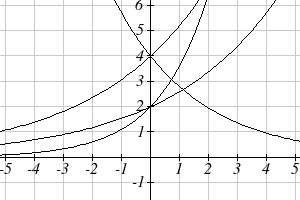
\includegraphics[width=0.5\textwidth]{img/chap1/sec1-6/image076.png}
\caption{}
\end{figure}
\solution The graph of $k(x)$ is the easiest to identify, since it is the only equation with a growth factor less than $1$, which will produce a decreasing graph. The graph of $h(x)$ can be identified as the only growing exponential function with a vertical intercept at the point $(0,4)$. The graphs of $f(x)$ and $g(x)$ both have a vertical intercept at $(0,2)$, but since $g(x)$ has a larger growth factor, we can identify it as the graph that is increasing faster.

\begin{figure}[!ht]
\centering
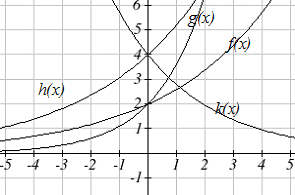
\includegraphics[width=0.5\textwidth]{img/chap1/sec1-6/image077.png}
\caption{}
\end{figure}

\end{example}

\subsection{Exercises}
\label{ssec:1-6-exercises}
\begin{enumerate}
\item[] Simplify each expression.
\item $x^3x^5$
\item $x^4x^2$
\item $(x^3)^4$
\item $(x^7)^2$
\item $(2x^2)^3x^4$
\item $(5x^4)^2 x^5$
\item $\frac{(3x^2)^2}{6x^3}$
\item $\frac{5x(4x)^2}{2x^2}$

\item[] Simplify, and rewrite without negative exponents.
\item $4x^{-3}$
\item $2x^{-5}$
\item $x^{-4}x^2$
\item $x^{-2}x$
\item $\frac{5x^{-3}}{2x^{-6}}$
\item $\frac{2x^{-4}}{6x^{-2}}$

\item[] Rewrite using negative or fractional exponents.
\item $\frac{4}{x^{5}}$
\item $\frac{4}{x^3}$
\item $3\sqrt{x}$
\item $\sqrt[4]{x}$
\item $\frac{4}{\sqrt[3]{x}}$
\item $\frac{1}{5\sqrt{x}}$

\item[] Rewrite as a radical.
\item $4x^{-1/2}$
\item $5x^{-1/3}$
\item $2x^{1/3}$
\item $5x^{3/2}$


  \item A population numbers 11,000 organisms initially and grows by 8.5\% each year.  Write an exponential model for the population.

  \item A population is currently 6,000 and has been increasing by 1.2\% each day.  Write an exponential model for the population.

\item A vehicle purchased for \$32,500 depreciates at a constant rate of 5\% each year. Determine the approximate value of the vehicle 12 years after purchase.

\item A business purchases \$125,000 of office furniture which depreciates at a constant rate of 12\% each year.  Find the residual value of the furniture 6 years after purchase.

\item If \$4,000 is invested in a bank account at an interest rate of 7 per cent per year, find the amount in the bank after 9 years if interest is compounded annually, quarterly, monthly, and continuously.

\item If \$6,000 is invested in a bank account at an interest rate of 9 per cent per year, find the amount in the bank after 5 years if interest is compounded annually, quarterly, monthly, and continuously.
Match each function with one of the graphs below.

\item $f(x) = 2(0.69)^x$
\item $f(x) = 2(1.28)^x$
\item $f(x) = 2(0.81)^x$
\item $f(x) = 4(1.28)^x$
\item $f(x) = 2(1.59)^x$
\item $f(x) = 4(0.69)^x$

If all the graphs to the right have equations with form $f(t) = a\cdot e^{kt}$,
\item Which graph has the largest value for $k$?
\item  Which graph has the smallest value for $k$?
\item  Which graph has the largest value for $a$?
\item  Which graph has the smallest value for $a$?
\end{enumerate}

\section{Logistic Functions}
\label{sec:logistic}

The (fictional) town of Sigmoidville has 5000 people. You and some friends design an app for residents of the town. Table \ref{tab:1-7-app} shows the number of downloads of the app over a span of 90 days.

\begin{table}[!ht]

	\centering
  \begin{tabular}{lrrrrrrrrrr}
    \toprule
    {\bf Day} ($t$)       & 0 & 10 & 20  & 30 & 40 & 50 & 60 & 70 & 80 & 90 \\
    \midrule
    {\bf Downloads} ($D$) & 16 & 52 & 166 & 491 & 1201 & 2127 & 2771 & 3049 & 3144 & 3174   \\
    \bottomrule
\end{tabular}
\caption{Total downloads, $D$, of the Sigmoidville app after $t$ days.}
\label{tab:1-7-app}
\end{table}

You notice that the download rate is slow, then rapid, then slow again. A plot of the data shows that this is indeed the case.

\begin{figure}[!ht]
	\centering
	\includegraphics[width = 0.6\textwidth]{img/chap1/sec1-7/1-7-app.png}
	\caption{Total downloads, $D$, of the Sigmoidville app after $t$ days.}
    \label{fig:1-7-app}
	\end{figure}


Why does this make sense? At first, only a few of you know about the app. As you tell others about the app, more will download it and they may tell others about the app as well, so download rates accelerate. However, there are only 5000 people in town and you don't expect anyone outside the town to download it, so eventually the market will be {\bf saturated}. Also, not everyone in town would want the app, so you may not get 5000 total downloads.

This situation is an example of {\bf bounded exponential growth}. In general, a curve called a {\bf logistic curve} models {\bf bounded exponential growth or decay}:  

\begin{definition}[Logistic Function]
  A {\bf logistic function}\index{Function!logistic} is a function of the form
  $$f(x) = \dfrac{L}{1+ae^{-bx}} \enspace .$$
    \begin{itemize}    
    \item If $b>0$, then $f(x)$ increases to the {\bf limiting value}\index{Limit} $L$.
    \item If $b<0$, then $f(x)$ decreases to 0.
    \end{itemize}
\end{definition}

Logistic models apply when there is a limit to the growth of some phenomenon. Examples of logistic models include the following.
    \begin{itemize}
    \item Product sales: an astute inventory manager will note when the total sales of an item have reached an {\bf inflection point} and will stop ordering that item to stock inventory.
    \item Population growth, where limited resources define a {\bf carrying capacity} of the population 
    \item The spread of an infectious disease.
    \end{itemize}

\begin{example} A (slightly simplified) {\bf best fit curve} can be found for the number of downloads of the Sigmoidville app after $t$ days: 
$$D(t) = \frac{3187}{1+201\cdot e^{-0.12t}} \text{ downloads after } t \text{ days.}$$
This tells us that we can expect a total of 3187 app downloads, so you have effectively reached the point of market saturation after 90 days and you can only expect a dozen or so more downloads.

\begin{figure}[!ht]
	\centering
	\includegraphics[width = 0.6\textwidth]{img/chap1/sec1-7/1-7-app-graph.png}
	\caption{Modeling the total downloads, $D$, of the Sigmoidville app after $t$ days.}
    \label{fig:1-7-app-graph}
	\end{figure}
\end{example}

You can model logistic growth with a group of people. One or two people are secretly, possibly randomly, chosen to be zombies. There are a number of ``rounds'' in which during each round, everyone shakes hands with another person. Zombies will give an extra squeeze or blink their eyes to indicate they are a zombie. If you shake hands with a zombie, you become a zombie yourself. Everyone must remember which round they became a zombie. Plot the cumulative number of zombies in each round. A plot of the data should look logistic, since there will be rapid growth initially, but as the proportion of zombies increases, there will be more occurrences of zombies shaking hands with other zombies, which does not increase the total number of zombies. Eventually, the whole group of people will be zombies.


\section{Logarithmic Functions}
\label{sec:log}

\section{Trigonometric Functions}
\label{sec:trig}

Most applied calculus texts skip {\bf trigonometric}\index{Functions!trigonometric} functions, but they are extremely powerful for modeling periodic or seasonal data. We will keep the treatment of these models very basic and intuitive, but independent from the rest of the text; it is optional. For the scientist, trigonometric functions are indispensable. However, for our purposes, we will focus our attention exclusively on two related functions: the {\bf sine}\index{Function!sine} and {\bf cosine}\index{Function!cosine} functions.

\subsection{Definitions}

% Insert definitions with graphs here.

A {\bf sine wave}\index{Sine} is of the form
\begin{equation}
\label{eq:sine}
f(x) = v + a \cdot \sin\left(\frac{2\pi(x-h)}{p}\right) \enspace .
\end{equation}
where $v$ is the {\bf vertical shift}\index{Shift!vertical} (mean of the data), $a$ is the {\bf amplitude}\index{Amplitude} of the wave (roughly the difference between the maximum and the mean of the data), $h$ is the {\bf horizontal shift}\index{Shift!horizontal} (where the data is at the mean and begins to rise to the maximum), and $p$ is the {\bf period}.

\subsection{Modeling with Sine Waves}

Consider the following table that we saw in Sections \ref{sec:models} and \ref{sec:polynomial} on the fuel oil usage of Plant W in 2016. One task that we were unable to complete before was to determine a model that would reflect the seasonality of the data. In other words, since the data represents a calendar year, we want a model that will oscillate and finish at the same output value as the output value of the beginning point. A {\bf trigonometric model}\index{Model!trigonometric} serves that very purpose.

\begin{table}[h!]
\centering
\begin{tabular}{l*{12}{c}}
\toprule
Month & Jan. & Feb. & Mar. & Apr. & May & June & July & Aug. & Sep. & Oct. & Nov. & Dec. \\
\midrule
Oil (gal) & 573.0 & 850.0 &  425.3 & 800.1  & 818.9 &  880.9 &  296.5 & 198.7 & 105.4 & 72.0 & ?? & 638.0\\
\bottomrule
\end{tabular}
\caption{Fuel Oil Usage at Plant W in 2016}
\label{tab:1-9-oil}
\end{table}

Given our data, we don't know the vertical shift, the amplitude, or the horizontal shift, but we do know the period. Since the input is in months and there are 12 months in a year, we choose $p = 12$ from \ref{eq:sine}. We then fit a sine wave to the data and get the following model.

If $m$ is the $m$th month of the year, then Plant W burned oil at a rate of
$$f(m) = 492.82 - 334.33\sin\left(\frac{2\pi(m+29.49)}{12} \right) \mbox{ gallons per month}$$
in 2016.

Graphing $y=f(m)$ with the scatter plot of Table \ref{tab:1-9-oil} gives us the following plot to verify that the model makes sense.
\begin{figure}[h!]
%\begin{wrapfigure}{R}{0.3\textwidth}
    \centering
    %\vspace{-20pt}
    \includegraphics[width=0.3\textwidth]{img/chap1/sec1-9/fig1-9-oil-curve.png}\\
    \caption{Fuel Oil Usage by Plant W in 2016 Fitted by a Sine Wave.}
    \label{fig:1-9-oil-curve}
%    \vspace{-20pt}
%\end{wrapfigure}
\end{figure}

\section{Combining Functions}
\label{sec:combining}


    % Uncomment individual sections in the files below when they are done.
    \chapter{The Derivative: Rates of Change of a Function}
\label{ch:derivatives}

\section{Slopes and Average Rates of Change}
\label{sec:slope}

Precalculus Idea: Slope and Rate of Change
The slope of a line measures how fast a line rises or falls as we move from left to right along the line. It measures the rate of change of the y-coordinate with respect to changes in the x-coordinate. If the line represents the distance traveled over time, for example, then its slope represents the velocity. In the figure, you can remind yourself of how we calculate slope using two points on the line:

slope
m=Slope from P to Q=riserun=y2-y1x2-x1=ΔyΔx
We would like to be able to get that same sort of information (how fast the curve rises or falls, velocity from distance) even if the graph is not a straight line. But what happens if we try to find the slope of a curve, as in the figure below?

slope
We need two points in order to determine the slope of a line. How can we find a slope of a curve, at just one point? The answer, as suggested in the figure, is to find the slope of the tangent line to the curve at that point. Most of us have an intuitive idea of what a tangent line is. Unfortunately, “tangent line” is hard to define precisely.

Definition (Secant Line)
A secant line is a line between two points on a curve

See the image below:

secant

\section{Tangent Lines and Instantaneous Rates of Change}
\label{sec:tangents}

%\section{Business Applications of Slope}
\label{sec:basic-apps}

Business and Economics Terms
Next we will delve more deeply into some business applications. To do that, we first need to review some terminology.

Suppose you are producing and selling some item. The profit you make is the amount of money you take in minus what you have to pay to produce the items. Both of these quantities depend on how many you make and sell. (So we have functions here.) Here is a list of definitions for some of the terminology, together with their meaning in algebraic terms and in graphical terms.

Cost
Your cost is the money you have to spend to produce your items.

Fixed Cost
The Fixed Cost (FC) is the amount of money you have to spend regardless of how many items you produce. FC can include things like rent, purchase costs of machinery, and salaries for office staff. You have to pay the fixed costs even if you don’t produce anything.

Total Variable Cost
The Total Variable Cost (TVC) for q items is the amount of money you spend to actually produce them. TVC includes things like the materials you use, the electricity to run the machinery, gasoline for your delivery vans, maybe the wages of your production workers. These costs will vary according to how many items you produce.

Total Cost
The Total Cost (TC, or sometimes just C) for q items is the total cost of producing them. It’s the sum of the fixed cost and the total variable cost for producing q items.

Average Cost
The Average Cost (AC) for q items is the total cost divided by q, or TCq. You can also talk about the average fixed cost, FCq, or the average variable cost, TVCq.

Marginal Cost
The Marginal Cost (MC) at q items is the cost of producing the next item. Really, it’s
MC(q)=TC(q+1)-TC(q).
In many cases, though, it’s easier to approximate this difference using calculus (see Example \ref{ex:2-7-11} below). And some sources define the marginal cost directly as the derivative,
MC(q)=TC′(q).
In this course, we will use both of these definitions as if they were interchangeable.

The units on marginal cost is cost per item.

Why is it okay that there are two definitions for Marginal Cost (and Marginal Revenue, and Marginal Profit)?

We have been using slopes of secant lines over tiny intervals to approximate derivatives. In this example, we’ll turn that around – we’ll use the derivative to approximate the slope of the secant line.

Notice that the “cost of the next item” definition is actually the slope of a secant line, over an interval of 1 unit:
MC(q)=C(q+1)-1=C(q+1)-11.
So this is approximately the same as the derivative of the cost function at q:
MC(q)=C′(q).
In practice, these two numbers are so close that there’s no practical reason to make a distinction. For our purposes, the marginal cost is the derivative is the cost of the next item.

\begin{example}
The table shows the total cost (TC) of producing q items.

Items, q	TC	0	\$20,000	100	\$35,000	200	\$45,000	300	\$53,000
What is the fixed cost?
When 200 items are made, what is the total variable cost? The average variable cost?
When 200 items are made, estimate the marginal cost.

\begin{solution}
  The fixed cost is \$20,000, the cost even when no items are made.
When 200 items are made, the total cost is \$45,000. Subtracting the fixed cost, the total variable cost is \$45,000 - \$20,000 = \$25,000.

The average variable cost is the total variable cost divided by the number of items, so we would divide the \$25,000 total variable cost by the 200 items made. \$25,000/200 = \$125. On average, each item had a variable cost of \$125.

We need to estimate the value of the derivative, or the slope of the tangent line at q=200. Finding the secant line from q=100 to q=200 gives a slope of
45,000-35,000200-100=100.
Finding the secant line from q=200 to q=300 gives a slope of
53,000-45,000300-200=80.
We could estimate the tangent slope by averaging these secant slopes, giving us an estimate of \$90/item.

This tells us that after 200 items have been made, it will cost about \$90 to make one more item.
\end{solution}\end{example}
 % Cut this section.
\section{The Derivative}
\label{sec:derivative}

\subsection{Derivative Concepts and Notation}

\begin{definition}
We can view the {\bf derivative}\index{Derivative} of a function, $f(x)$ in several different equivalent ways. Here are a three of them. The derivative of $f(x)$ at a point $(a, f(a))$ is:
    \begin{itemize}
    \item the instantaneous rate of change of $f(x)$ at $x=a$, 
    \item the slope of the tangent line to the graph of $f(x)$ at the point $(a,f(a))$, and
    \item the slope of the curve $y=f(x)$ at the point $(a,f(a))$.
    \end{itemize}
\end{definition}

We've been acting as if derivatives exist everywhere for every function. This is true for most of the functions that you will run into in this textbook. But there are some common places where the derivative doesn't exist.

\begin{definition}
A function, $f(x)$, is called {\bf differentiable}\index{Differentiable} at the point $(a,f(a))$ if its derivative exists at $x=a$.
\end{definition}

Remember that the derivative is the slope of the tangent line to the curve. That's what to think about.

Where can a slope not exist? If the tangent line is vertical, the derivative will not exist.

\begin{example}
Show that $f(x)=\sqrt[3]{x}=x^{1/3}$ is not differentiable at $x=0$.

\begin{solution} From the graph in Figure \ref{fig:2-3-cuberoot}, we can see that the tangent line to $y=\sqrt[3]{x}$ at $x=0$ is vertical with undefined slope, which is why the derivative does not exist at $x=0$.

\begin{figure}[!ht]
  \centering
    \includegraphics[width=0.4\textwidth]{img/chap2/image037.png}
    \caption{$f(x)=\sqrt[3]{x}$}
    \label{fig:2-3-cuberoot}
\end{figure}
\end{solution}\end{example}

Where can a tangent line not exist?

If there is a sharp corner (cusp)\index{Cusp} in the graph, the derivative will not exist at that point because there is no well-defined tangent line (a teetering tangent, if you will).

If there is a discontinuity\index{Discontinuity} in the graph (a jump, a break, a hole in the graph, or a vertical asymptote), the tangent line will be different on either side and the derivative will not exist at that point.

\begin{example}
Show that $f(x)=|x|$ is not differentiable at $x=0$.

\begin{solution} On the left side of the graph in Figure \ref{fig:2-3-absx}, the slope of the line is $-1$. On the right side of the graph, the slope is $1$. There is no well-defined tangent line at the sharp corner at $x=0$, so the function $|x|$ is not differentiable at that point.

\begin{figure}[!ht]
  \centering
    \includegraphics[width=0.4\textwidth]{img/chap2/image038.png}
    \caption{$f(x)=|x|$}
    \label{fig:2-3-absx}
\end{figure}
\end{solution}\end{example}


\begin{definition}
When we find the derivative of a function, or take the derivative of a function, we say that we {\bf differentiate}\index{Differentiate} the function.
\end{definition}

\paragraph*{Notation for the Derivative}
Calculus was invented by Leibniz\index{Leibniz, Gottfried} and Newton\index{Newton, Isaac}, but it was developed by many more throughout the subsequent centuries. Many developed their own notation for the derivative of a function. The notation developed by Leibniz and Joseph-Louis Lagrange\index{Lagrange, Joseph-Louis} are the most convenient and most used. 

The derivative of $y=f(x)$, with respect to $x$, is written in many different ways:
\begin{itemize}
    \item $f'(x)$: ``$f$ prime of $x$'',
    \item $y'$: ``$y$ prime,''
    \item $\dfrac{dy}{dx}$: ``$d$ $y$ $d$ $x$,''  
    \item $\dfrac{df}{dx}$: ``$d$ $f$ $d$ $x$,'' or
    \item $\dfrac{d}{dx}f(x)$: ``$d$ $d$ $x$ of $f$ of $x$.''
\end{itemize}
The notation that resembles a fraction is called {\bf Leibniz notation}\index{Leibniz notation}. It displays not only the name of the function ($f$ or $y$), but also the name of the variable (in this case, $x$). It looks like a fraction because the derivative is a slope. In fact, this is simply $\dfrac{\Delta y}{\Delta x}$ written in Roman letters instead of Greek letters. The nuance here is that $\Delta v$\index{Delta} represents a finite difference of some variable $v$, whereas $dv$ represents an {\bf infinitesimal}\index{Infinitesimal} difference of a variable $v$. An infinitesimal difference would be a difference that is infinitely small, but not 0. That may sound like an oxymoron, but until about 1850, calculus was developed using infinitesimal differences, also called {\bf differentials}\index{Differential}. 

The best way to understand differentials is with an analogy: $1:\infty::dx:1$. Suppose you had a bin with an infinite number of balls and you throw one ball in. You still throw in a ball, but the total quantity of balls in the bin is unchanged. In the same way, if you have a line that is one inch long and you add on a line of length $dx$ inches, then the line is still one inch long, despite ``lengthening'' the line by $dx$.
 
\paragraph*{Looking Ahead}
We will figure out ways to compute exact values of derivatives from many kinds of functions in Sections \ref{sec:algderiv}-\ref{sec:chain}. If the function is given to you as a table or graph, you will still need to approximate the derivative of the function this way.

This is the foundation for the rest of this chapter. It's remarkable that such a simple idea (the slope of a tangent line) and such a simple definition (for the derivative $f'(x)$) will lead to so many important ideas and applications.

\subsection{The Derivative as a Function}
We now know how to find (or at least approximate) the derivative of a function for any $x$-value. This means that we can think of the derivative as a function too. That is the origin of the term ``derivative.'' The derivative of a function is a function that is derived from that function. The input of the derivative is the same as the function, but the output is the value of the derivative at that $x$ value and the units reflect the rate of change concept.

\begin{example}
Below is the graph of a function $y=f(x)$. We can use the information in the graph to fill in a table showing values of $f'(x)$:
\begin{figure}[!ht]
  \centering
    \includegraphics[width=0.4\textwidth]{img/chap2/image023.png}
    \caption{$y=f(x)$}
    \label{fig:2-3-fx}
\end{figure}

\begin{solution} At various values of $x$, draw your best guess at the tangent line and measure its slope. You might have to extend your lines so you can read some points. In general, your estimate of the slope will be better if you choose points that are easy to read and far away from each other. Here are estimates for a few values of $x$ (parts of the tangent lines used are shown above in the graph):
\begin{table}[ht!]
\begin{centering}
\begin{tabular}{ccc}
\toprule
$x$ &   $y=f(x)$    &	$f'(x)$\\
\midrule
0   &	0 &	1	\\
1   &	1 &	0	\\
2   &	0 &	$-1$  \\
3   &  $-1$ &	0	\\
3.5 &	0 &	2   \\
\bottomrule
\end{tabular}
\caption{Table of inputs, outputs, and derivatives of $f(x)$.}
\label{tab:2-3-deriv}
\end{centering}
\end{table}
Based on this, we can estimate the values of $f'(x)$ at some non-integer values of $x$ too: $f'(0.5)\approx   0.5$ and $f'(1.3)\approx   -0.3$.
\begin{figure}[!ht]
  \centering
    \includegraphics[width=0.4\textwidth]{img/chap2/image024.png}
    \caption{Slope of $y=f(x)$}
    \label{fig:2-3-fprimex}
\end{figure}
We can even think about entire intervals. For example, if $0<x<1$, then $f(x)$ is increasing; all the slopes are positive, and so $f'(x)>0$.

The values of $f'(x)$ definitely depend on the values of $x$, and $f'(x)$ is a function of $x$. We can use the results in the table to help sketch the graph of $f'(x)$.

\end{solution}\end{example}
\begin{example}
Figure \ref{fig:2-3-ht} shows the graph of the height, $h(t)$, of a rocket $t$ seconds after liftoff.

\begin{figure}[!ht]
  \centering
    \includegraphics[width=0.4\textwidth]{img/chap2/image025.png}
    \caption{$y=h(t)$}
    \label{fig:2-3-ht}
\end{figure}
Sketch the graph of the velocity of the rocket at time $t$. (Velocity is the derivative of the height function, so it is the slope of the tangent to the graph of position or height.)

\begin{solution} We can estimate the slope of the function at several points. The graph in Figure \ref{fig:2-3-hprime} shows the velocity of the rocket. This is $v(t)=h'(t)$.

\begin{figure}[!ht]
  \centering
    \includegraphics[width=0.4\textwidth]{img/chap2/image026.png}
    \caption{$y=h(x)$ and $y=h'(x)$}
    \label{fig:2-3-hprime}
\end{figure}
\end{solution}
\end{example}

\subsection{Interpreting the Derivative}
So far we have emphasized the derivative as the slope of the line tangent to a graph. That interpretation is very visual and useful when examining the graph of a function, and we will continue to use it. Derivatives, however, are used in a wide variety of fields and applications, and some of these fields use other interpretations. The following are a few interpretations of the derivative that are commonly used.

\paragraph*{General}

{\bf Rate of Change:} $f'(x)$ is the rate of change of the function at $x$. If the units for $x$ are years and the units for $f(x)$ are people, then the units for $\frac{df}{dx}$ are people per year, a rate of change in population.

\paragraph*{Graphical}

{\bf Slope:} $f'(x)$ is the slope of the line tangent to the graph of $f(x)$ at the point $(x,f(x))$.

\paragraph*{Physical}

{\bf Velocity:} If $f(x)$ is the position of an object at time $x$, then $f'(x)$ is the {\bf velocity}\index{Velocity} of the object at time $x$. If the units for $x$ are hours and $f(x)$ is distance measured in miles, then the units for $f'(x)=\frac{df}{dx}$ are miles per hour, which is a measure of velocity.

{\bf Acceleration:} If $f(x)$ is the velocity of an object at time $x$, then $f'(x)$ is the {\bf acceleration}\index{Acceleraton} of the object at time $x$. If the units are for $x$ are hours and $f(x)$ has the units miles per hour, then the units for the acceleration $f'(x)=\frac{df}{dx}$ are miles per hour per hour, or miles per hour$^2$.

\paragraph*{Business}

{\bf Marginal Cost}\index{Marginal cost}\index{Cost!marginal}, {\bf Marginal Revenue}\index{Marginal revenue}\index{Revenue!marginal}, and {\bf Marginal Profit}\index{Marginal profit}\index{Profitmarginal}: We introduced marginal cost in Section \ref{ssec:marginalcost} and marginal revenue and profit are defined in a similar way. In business contexts, the word ``marginal'' usually means the derivative or rate of change of some function. 

Therefore, {\bf marginal revenue}, $MR(n)$ is the additional revenue from selling one more item once we have already sold $n$ item. Just as with marginal cost, we will use both this definition and the derivative definition.
$$MR(n) = R(n+1)-R(n) \approx R'(n) \enspace.$$

{\bf Marginal profit} is the additional profit from selling one more item once we have already sold $n$ items. 
$$MP(n) = P(n+1)-P(n) \approx P'(n) \enspace.$$

If $f(x)$ is the cost to produce $x$ bicycles and the units for $f(x)$ are dollars, then the units for $f'(x)=\frac{df}{dx}$ are dollars per bicycle, the cost per bicycle.

One of the strengths of calculus is that it provides a unity and economy of ideas among diverse applications. The vocabulary and problems may be different, but the ideas and even the notations of calculus are still useful.

\subsection{Graphical Interpretations of the Basic Business Math Terms}
%Illustration
Figure \ref{fig:2-3-trandtc} shows graphs of $TR = R(q)$ and $TC = C(q)$ for producing and selling a certain item. The horizontal axis is the number of items, in thousands. The vertical axis is the number of dollars, also in thousands.

\begin{figure}[!ht]
  \centering
    \includegraphics[width=0.4\textwidth]{img/chap2/image035.png}
    \caption{Total Revenue ($TR$) and Total Cost ($TC$) versus $q$ items.}
    \label{fig:2-3-trandtc}
\end{figure}
First, notice how to find the fixed cost and variable cost from the graph here. The fixed cost, $FC$, is the $y$-intercept of the $TC$ graph. ($FC=C(0)$.) The graph of variable costs would have the same shape as the graph of $TC$, shifted down.

Marginal cost for $q$ items is $MC(q)=C(q+1)-C(q)$, but that's impossible to read on this graph. How could you distinguish between $C(4022)$ and $C(4023)$? On this graph, that interval is too small to see, and our best guess at the secant line is actually the tangent line to the $TC$ curve at that point. (This is the reason we want to have the derivative definition handy.)
\begin{itemize}[label={}]
    \item $MC(q)$ is the slope of the tangent line to the $TC$ curve at the point $(q, C(q))$.
    \item $MR(q)$ is the slope of the tangent line to the $TR$ curve at the point $(q, R(q))$.
\end{itemize}
Profit is the distance between the $TR$ and $TC$ curves. If you experiment with a clear ruler, you'll see that the biggest profit occurs exactly when the tangent lines to the $TR$ and $TC$ curves are parallel. This is the rule that profit is maximized when $MR=MC$ which we'll explore in Section \ref{sec:app-opt}.

\begin{example}
Suppose the demand for widgets is $D(p)=\frac{1}{p}$, where $D$ is the quantity of widgets, in thousands, at a price of $p$ dollars. Approximate and interpret the derivative of $D$ at $p=\$3$.

\begin{solution} We can approximate $D'(3)$ by looking at a table, Table \ref{tab:2-3-Dprime}, of secant line slopes through the points $(3, D(3)) = \left(3, \frac{1}{3}\right)$ and $(3+\Delta p, D(3+\Delta p))$, where $\Delta p$ gets closer to $0$.

\begin{table}[ht!]
\begin{centering}
\begin{tabular}{lll}
\toprule
$\Delta p$ & $D(3+\Delta p)$ & $\dfrac{D(3+\Delta p)-D(3)}{\Delta p}$ \\
\midrule
1        & $\dfrac{1\mathstrut}{3+1\mathstrut} = 0.25$                & $\dfrac{D(4)     -D(3)}{1}     \approx -0.083333$ \\
0.1      & $\dfrac{1\mathstrut}{3+0.1\mathstrut} \approx 0.322581$    & $\dfrac{D(3.1)   -D(3)}{0.1}   \approx -0.107527$ \\
0.01     & $\dfrac{1\mathstrut}{3+0.01\mathstrut} \approx 0.332226$   & $\dfrac{D(3.01)  -D(3)}{0.01}  \approx -0.110742$ \\
0.001    & $\dfrac{1\mathstrut}{3+0.001\mathstrut} \approx 0.333222$  & $\dfrac{D(3.001) -D(3)}{0.001} \approx -0.111074$ \\
0.0001   & $\dfrac{1\mathstrut}{3+0.0001\mathstrut} \approx 0.333322$ & $\dfrac{D(3.0001)-D(3)}{0.0001}\approx -0.111107$ \\
\bottomrule
\end{tabular}
\caption{Average rate of change of demand approaching $D'(3)$.}
\label{tab:2-3-Dprime}
\end{centering}
\end{table}
Based on this, the quantities in the last column appear to be approaching $-0.1111\ldots$, which is $\frac{-1}{9}$. Later, we will show that that is indeed true. Since $D(p)$ has units ``thousands of widgets'' and the units for $p$ is ``dollars,'' the units for $D'(3)$ will be thousands of widgets per dollar. Therefore, $D'(3) \approx -0.111$ thousand widgets per dollar, or $-111$ widgets per dollar. This shows how the demand for widgets will change as the price increases.

Specifically, $D'(3)\approx -111$ widgets per dollar tells us that when the price of a widget is $\$3$, then the demand for widgets will decrease by about 111 widgets for every dollar the price increases.
\end{solution}\end{example} 

In the next section, we will lay the theoretical foundation to establish a rigorous and precise definition of the derivative of a function.



\section{Limits of Functions}
\label{sec:limits}

\subsection{Limits}
In Section \ref{sec:tangents}, we saw that as the interval over which we calculated got smaller, the secant slopes approached the tangent slope. The {\bf limit}\index{Limit} gives us better language with which to discuss the idea of ``approaches.''
\begin{wrapfigure}{R}{0.25\textwidth}
  \vspace{-20pt}
  \centering
    \includegraphics[width=0.24\textwidth]{img/chap2/image011.png} 
\caption{The limit of $f(x)$ as $x\to c$ is $L$.}
\label{fig:2-4-limits}
\vspace{-20pt}
\end{wrapfigure}
The limit of a function describes the behavior (i.e., output) of the function when the variable is near, but not necessarily equal to, a specified number. (See Figure \ref{fig:2-4-limits}.)

\begin{definition}[Limit]
If the values of $f(x)$ get closer and closer, as close as we want, to one single number $L$, as we take values of $x$ very close to (but not equal to) a number $c$, then we say, ``the {\bf limit} of $f(x)$ as $x$ approaches $c$ is $L$'' and we write
$$\lim_{x\to c}f(x)=L \enspace .$$
The symbol ``$\to$'' means ``approaches'' or, less formally, ``gets very close to.''
\end{definition}
This definition of the limit isn't stated as formally as it could be, but it is sufficient for our purposes in this textbook.

{\bf Note:}
    \begin{itemize}[label={}]
    \item $f(c)$ is a single number that describes the behavior (value) of $f(x)$ at the point $x=c$.
    \item $\displaystyle\lim_{x\to c}f(x)$ is a single number that describes the behavior of $f(x)$ near, but NOT at, the point $x=c$.
    \item If we have a graph of $f(x)$ near $x = c$, then it is usually easy to determine $\displaystyle\lim_{x\to c}f(x)$.
    \end{itemize}

\begin{example}
Use the graph of $y=f(x)$ in Figure \ref{fig:2-4-limit-ex} to determine the following limits.
\begin{figure}[!ht]
    \centering
    \includegraphics[width=0.4\textwidth]{img/chap2/image012.png}
    \label{$y=f(x)$}
    \label{fig:2-4-limit-ex}
\end{figure}

\begin{enumerate}[label=(\alph*)]
  \item $\displaystyle\lim_{x\to 1}f(x)$

  \begin{solution}
When $x$ is very close to 1, the values of $f(x)$ are very close to $y=2$. In this example, it happens that $f(1)=2$, but that is irrelevant for the limit. The only thing that matters is what happens for $x$ close to 1 but $x\neq 1$.
    \end{solution}
  \item $\displaystyle\lim_{x\to 2}f(x)$

  \begin{solution}
$f(2)$ is undefined, but we only care about the behavior of $f(x)$ for $x$ close to 2 but not equal to 2. When $x$ is close to 2, the values of $f(x)$ are close to 3. If we restrict $x$ close enough to 2, the values of $y$ will be as close to 3 as we want, so $\displaystyle\lim_{x\to 2}f(x)=3$.
    \end{solution}
  \item $\displaystyle\lim_{x\to 3}f(x)$

  \begin{solution}
When $x$ is close to 3 (or ``as $x$ approaches the value 3''), the values of $f(x)$ are close to 1 (or ``approach the value 1''), so $\displaystyle\lim_{x\to 3}f(x)=1$. For this limit it is completely irrelevant that $f(3)=2$. We only care about what happens to $f(x)$ for $x$ close to and not equal to 3.
    \end{solution}
  \item $\displaystyle\lim_{x\to 4}f(x)$

  \begin{solution}
This one is harder and we need to be careful. When $x$ is close to 4 and slightly less than 4 ($x$ is just to the left of 4 on the $x$-axis), then the values of $f(x)$ are close to 2. But if $x$ is close to 4 and slightly larger than 4 then the values of $f(x)$ are close to 3. If we only know that $x$ is very close to 4, then we cannot say whether $y=f(x)$ will be close to 2 or close to 3. It depends on whether $x$ is on the right or the left side of 4. In this situation, the $f(x)$ values are not close to a single number so we say $f(x)$ does not exist. It is irrelevant that $f(4)=1$. The limit, as $x$ approaches 4, would still be undefined if $f(4)$ was 3, 2, or anything else.
    \end{solution}
\end{enumerate}
\end{example}

We can also explore limits using tables and using algebra.

\begin{example}
Find $\displaystyle\lim_{x\to 1}f(x)$, where $f(x) = \dfrac{2x^2-x-1}{x-1}$.

\begin{solution} You might try to evaluate at $x=1$, but $f(x)$ is not defined at $x=1$. It is tempting, but incorrect, to conclude that this function does not have a limit as $x$ approaches 1.

{\bf Using tables:} Trying some ``test'' values for $x$ which get closer and closer to 1 from both the left and the right, we get the following table. 
\begin{table}[ht!]
\begin{centering}
\begin{tabular}{ll||ll}
\toprule
$x$ & 	$f(x)$ & $x$ &	$f(x)$\\					
\midrule
0.9	        & 2.82      & 1.1       & 3.2 \\
0.9998      & 2.9996	& 1.003	    & 3.006 \\
0.999994    & 2.999988	& 1.0001	& 3.0002 \\
0.9999999   & 2.9999998	& 1.000007	& 3.000014 \\
$\to 1$     & $\to 3$   & $\to 1$   & $\to 3$ \\
\bottomrule
\end{tabular}
\caption{Finding the limit of $f(x)$ as $x\to 1$}
\label{tab:2-4-limitex}
\end{centering}
\end{table}
Table \ref{tab:2-4-limitex} suggests that $\displaystyle\lim_{x\to 1}f(x) = 3$. This is not a proof, but is very convincing. A proof would require algebraic techniques.

{\bf Using algebra:} We can prove this result by noting that
$$f(x)=\dfrac{2x^2-x-1}{x-1}=\frac{(2x+1)(x-1)}{x-1}=2x+1 \enspace ,$$
as long as $x\neq 1$. (If $x\neq 1$, then $x-1\neq 0$, so it is valid to divide the numerator and denominator by the factor $x-1$.) The ``$x\to 1$'' part of the limit means that $x$ is close to 1 but not equal to 1, so our division step is valid and
$$\lim_{x\to 1}\dfrac{2x^2-x-1}{x-1}=\lim_{x\to 1}2x+1=3 \enspace,$$
which is our answer.

{\bf Using a graph:} We can graph $y=f(x)=\dfrac{2x^2-x-1}{x-1}$ for $x$ close to 1.
\begin{figure}[!ht]
    \centering
    \includegraphics[width=0.4\textwidth]{img/chap2/image013.png}
    \label{$y=f(x)$ near $x=1$}
    \label{fig:2-4-limit-zoom}
\end{figure}
Notice that whenever $x$ is close to 1, the values of $y=f(x)$ are close to 3. Since $f$ is not defined at $x=1$, the graph has a hole above $x=1$, but we only care about what $f(x)$ is doing for $x$ close to but not equal to 1. Therefore,
$$\lim_{x\to 1}\dfrac{2x^2-x-1}{x-1}=\lim_{x\to 1}2x+1=3 \enspace.$$
\end{solution}\end{example}

\subsection{One Sided Limits}
Sometimes, what happens to us at a place depends on the direction we use to approach that place. If we approach Niagara Falls from the upstream side, then we will be 182 feet higher and have different worries than if we approach from the downstream side. Similarly, the values of a function near a point may depend on the direction we use to approach that point.

\definition[Left and Right Limits]
The {\bf left limit}\index{Limit!left} of $f(x)$ as $x$ approaches $c$ is $L$ if the values of $f(x)$ get as close to $L$ as we want when $x$ is very close to and left of $c$ (i.e., $x<c$). We write:
$$\lim_{x\to c^-}f(x)=L \enspace .$$
The{\bf right limit}\index{Limit!right} of $f(x)$ as $x$ approaches $c$ is $L$ if the values of $f(x)$ get as close to $L$ as we want when $x$ is very close to and right of $c$ (i.e., $x>c$). We write
$$\lim_{x\to c^+}f(x)=L \enspace .$$
\begin{example}
Evaluate the one sided limits of the function $f(x)$ graphed below at $x=0$ and $x=1$.

[graph]

\begin{solution} As $x$ approaches 0 from the left, the value of the function is getting closer to 1, so $\displaystyle\lim_{x\to 0^-}f(x)=1$.
As $x$ approaches 0 from the right, the value of the function is getting closer to 2, so $\displaystyle\lim_{x\to 0^+}f(x)=2$.
Notice that since the limit from the left and limit from the right are different, the general limit, $\displaystyle\lim_{x\to 0}f(x)$, does not exist.

At $x$ approaches 1 from either direction, the value of the function is approaching 1, so
$$\lim_{x\to 1^-}f(x)=\lim_{x\to 1^+}f(x)=\lim_{x\to 1}f(x)=1 \enspace.$$
\end{solution}\end{example}

\subsection{Continuity}
\label{ssec:continuity}
A function that is ``friendly'' and doesn't have any breaks or jumps in it is called {\bf continuous}\index{Continuous}. More formally,

\begin{definition}[Continuity at a Point]
A function $f(x)$ is {\bf continuous} at $x=a$ if and only if:
    \begin{enumerate}
    \item $f(a)$ exists,
    \item $\displaystyle\lim_{x\to a}f(x)$ exists, and 
    \item $\displaystyle\lim_{x\to a}f(x)=f(a)$.
    \end{enumerate}
\end{definition}
The graph below illustrates some of the different ways a function can behave at and near a point, and the table contains some numerical information about the function and its behavior.

graph 
\begin{table}[ht!]
\begin{centering}
\begin{tabular}{ccc}
\toprule
$a$	& $f(a)$ &	$\displaystyle\lim_{x\to a}f(x)$ \\		
\midrule
1 &	2 & 2	\\
2 & 1 &	2\\
3 & 2 &	Does not exist (DNE)	\\
4 & Undefined &	2\\
\bottomrule
\end{tabular}
%\caption{}
%\label{tab:2-4-limitex2}
\end{centering}
\end{table}
	
Based on the information in the table, we can conclude that $f(x)$ is continuous at 1 since $\displaystyle\lim_{x\to 1}f(x)=2=f(1)$. We can also conclude from the information in the table that $f(x)$ is not continuous at 2, 3, or 4, because $\displaystyle\lim_{x\to 2}f(x)\neq f(2)$, $\displaystyle\lim_{x\to 3} f(x)\neq f(3)$, and $\displaystyle\lim_{x\to 4} f(x)\neq f(4)$.

The behaviors at $x=2$ and $x=4$ exhibit a hole in the graph, sometimes called a {\bf removable discontinuity}\index{Discontinuity!removeable}, since the graph could be made continuous by changing the value of a single point. The behavior at $x=3$ is called a {\bf jump discontinuity}\index{Discontinuity!jump} or {\bf step discontinuity}\index{Discontinuity!step}, since the graph jumps between two values. Jump discontinuities and vertial asymptotes are both {\bf nonremovable discontinuities}\index{Discontinuity!nonremoveable} because they cannot be fixed by changing the value of a single point.

So which functions are continuous? It turns out pretty much every function you've studied is continuous where it is defined: polynomial, radical, rational, exponential, and logarithmic functions are all continuous where they are defined. Moreover, any sum, difference, or product of continuous functions is also continuous.

This is helpful, because the definition of continuity says that for a continuous function, $\displaystyle\lim_{x\to a}f(x)=f(a)$. That means for a continuous function, we can find the limit by direct substitution (evaluating the function) if the function is continuous at $a$.

\begin{example}
Evaluate using continuity, if possible:
    \begin{enumerate}[label=(\alph*)]
    \item $\displaystyle\lim_{x\to 2}x^3-4x$

    \begin{solution} The given function is a polynomial, so it is defined for all values of $x$. Therefore, we can find the limit by direct substitution:
    $$\lim_{x\to 2}x^3-4x = 2^3-4(2) = 0 \enspace.$$
    \end{solution}
    \item $\displaystyle\lim_{x\to 2}\frac{x-4}{x+3}$

    \begin{solution} 
    The given function is rational. It is not defined at $x = -3$, but we are taking the limit as $x$ approaches 2, and the function is defined at that point, so we can use direct substitution:
    $$\lim_{x\to 2}\frac{x-4}{x+3} = \frac{2-4}{2+3}=-\frac{2}{5} \enspace .$$
    \end{solution}
    \item $\displaystyle\lim_{x\to 2} \frac{x-4}{x-2}$

    \begin{solution} 
    This function is not defined at $x = 2$, so is not continuous at $x = 2$. We cannot use direct substitution. There is also no factor of $x-2$ in the numerator, so the $x-2$ in the denominator cannot be canceled out to remove the discontinuity. Therefore, the limit does not exist.
    \end{solution}
\end{enumerate}
\end{example}

\section{Finding Derivatives Algebraically}
\label{sec:algderiv}

Formal Algebraic Definition
f′(x)=limh→0f(x+h)-f(x)h
Practical Definition
The derivative can be approximated by looking at an average rate of change, or the slope of a secant line, over a very tiny interval. The tinier the interval, the closer this is to the true instantaneous rate of change, slope of the tangent line, or slope of the curve.

\begin{example}
Find the slope of the tangent line to f(x)=1x at x=3.

\begin{solution} The slope of the tangent line is the value of the derivative f′(3). f(3)=13 and f(3+h)=13+h, so, using the formal limit definition of the derivative,
f′(3)=limh→0f(3+h)-f(3)h=limh→013+h-13h.
We can simplify by giving the fractions a common denominator:
limh→013+h-13h=======limh→013+h⋅33-13⋅3+h3+hhlimh→039+3h-3+h9+3hhlimh→03-(3+h)9+3hhlimh→03-3-h9+3hhlimh→0-h9+3hhlimh→0-h9+3h⋅1hlimh→0-19+3h
and the evaluate using direct substitution:
limh→0-19+3h=-19+3(0)=-19.
Thus, the slope of the tangent line to f(x)=1x at x=3 is -19.
\end{solution}\end{example}

\begin{example}
Find ddx(2x2-4x-1).

\begin{solution} Setting up the derivative using a limit,
f′(x)=limh→0f(x+h)-f(x)h.
We will start by simplifying f(x+h) by expanding:
f(x+h)===2(x+h)2-4(x+h)-12(x2+2xh+h2)-4(x+h)-12x2+4xh+2h2-4x-4h-1
Now finding the limit:
f′(x)======limh→0f(x+h)-f(x)hlimh→0(2x2+4xh+2h2-4x-4h-1)-(2x2-4x-1)hlimh→02x2+4xh+2h2-4x-4h-1-2x2+4x+1h(Substitute in the formulas.)limh→04xh+2h2-4hh(Now simplify.)limh→0h(4x+2h-4)h(Factor out the h, then cancel.)limh→0(4x+2h-4)
We can find the limit of this expression by direct substitution:
f′(x)=limh→0(4x+2h-4)=4x-4
Notice that the derivative depends on x, and that this formula will tell us the slope of the tangent line to f at any value x. For example, if we wanted to know the tangent slope of f at x=3, we would simply evaluate: f′(3)=4(3)-4=8.
\end{solution}\end{example}
A formula for the derivative function is very powerful, but as you can see, calculating the derivative using the limit definition is very time consuming. In the next section, we will identify some patterns that will allow us to start building a set of rules for finding derivatives without needing the limit definition.

\section{Sum, Difference, and Constant Multiple Rules}
\label{sec:power}

In the next few sections, we'll get the derivative rules that will let us find formulas for derivatives when our function comes to us as a formula. 

\subsection{Sum and Difference}
Given two functions, $f(x)$ and $g(x)$, what can be said about the derivative of their sum? Think about it. What should we expect for the slope of the curve $y = f(x)+g(x)$ or the curve $y=f(x) - g(x)$? We can prove the following result using the limit definition of the derivative, but it should make intuitive sense that the slope of a sum is the sum of the slopes.

\begin{theorem}[Sum and Difference Rule\index{Sum and difference rule}\index{Derivative rules!Sum and difference rule}]
\label{thm:sumdiffderiv}
If $f(x)$ and $g(x)$ are differentiable, then 
    $$\dfrac{d}{dx}(f(x) \pm g(x))=f'(x) \pm g'(x) \enspace .$$
\end{theorem}

\subsection{Constant Multiples}
Given a single function, $f(x)$, we have $2f(x) = f(x) + f(x)$ and $3f(x) = f(x) + f(x) + f(x)$, so it would make sense that the slope of $y=k\cdot f(x)$ is $k$ times the slope of $y=f(x)$. This too, can be proved using the limit definition of the derivative. We often say that when taking the derivative of a multiple of a function, that ``constants come along for the ride.'' 

\begin{theorem}[Constant Multiple Rule\index{Constant multiple rule}\index{Derivative rules!Constant multiple rule}]
\label{thm:constmultderiv}
If $f(x)$ is differentiable and $k$ is a real number, then
$$\dfrac{d}{dx}(k\cdot f(x))=k\cdot f'(x) \enspace .$$
\end{theorem}

\subsection{Exercises}
\begin{enumerate}
    \item Prove Theorem \ref{thm:sumdiffderiv} using the limit definition of the derivative, Definition \ref{def:deriv}.
    \item Prove Theorem \ref{thm:constmultderiv} using the limit definition of the derivative, Definition \ref{def:deriv}.
\end{enumerate}


\section{The Power Rule}
\label{sec:power}

\section{Exponential and Logarithmic Functions}
\label{sec:explogderiv}

\begin{theorem}
{\bf Exponential Functions}
$$\dfrac{d}{dx}e^x=e^x$$
$$\dfrac{d}{dx}a^x=\ln(a)a^x$$
{\bf Logarithmic Functions}
$$\dfrac{d}{dx}\ln(x)=\dfrac{1}{x}$$
$$\dfrac{d}{dx}\log_b(x)=\dfrac{1}{x\ln(b)}\enspace , b>0, b\neq 1 $$
\end{theorem}

\section{The Product and Quotient Rules}
\label{sec:prod-quot}

% Dollar-cost averaging example. Invest $100 per month and price of asset goes up \$10 per month. How fast does the investment grow?

The basic rules will let us tackle simple functions. But what happens if we need the derivative of a combination of these functions?

\begin{example}
  \label{ex:2-8-1}
Find the derivative of $h(x)=(4x^3-11)(x+3)$.

\begin{solution} This function is not a simple sum or difference of polynomials. It's a product of polynomials. We can simply multiply it out to find its derivative:
\begin{align*}
		h(x) &= \left(4x^3-11\right)(x+3)\\
		 &= 4x^4-11x+12x^3-33\\
		h'(x) &= 16x^3-11+36x^2
	\end{align*}
\end{solution}\end{example}

Now suppose we wanted to find the derivative of
$$f(x)=\left(4x^5+x^3-1.5x^2-11\right)\left(x^7-7.25x^5+120x+3\right)$$)
This function is not a simple sum or difference of polynomials. It's a product of polynomials. We could 'simply' multiply it out to find its derivative as before -- who wants to volunteer? Nobody?

We'll need a rule for finding the derivative of a product so we don't have to multiply everything out.

It would be great if we can just take the derivatives of the factors and multiply them, but unfortunately that won't give the right answer. To see that, consider finding derivative of $h(x)=(4x^3-11)(x+3)$. We already worked out the derivative, it is $h'(x)=16x^3-11+36x^2$. What if we try differentiating the factors and multiplying them? We'd get $h'(x)=(12x^2)(1)=12x^2$, which is radically different from the correct answer.

In other words, the derivative of a product is not the product of the derivatives.

The rules for finding derivatives of products and quotients are a little complicated, but they save us the much more complicated algebra we might face if we were to try to multiply things out. They also let us deal with products where the factors are not polynomials. We can use these rules, together with the basic rules, to find derivatives of many complicated looking functions.

\subsection{Derivative Rules: Product and Quotient Rules}
\begin{theorem}[Product Rule\index{Product Rule}]
If $f(x)$ and $g(x)$ are differentiable, then
$\dfrac{d}{dx}\left( f(x)\cdot g(x) \right)=f'(x)\cdot g(x)+f(x)\cdot g'(x) \enspace .$
\end{theorem}

The derivative of the first factor times the second left alone, plus the first left alone times the derivative of the second.

The Product Rule can extend to a product of several functions; the pattern continues -- take the derivative of each factor in turn, multiplied by all the other factors left alone, and add them up:
$$\dfrac{d}{dx} f(x)\cdot g(x)\cdot h(x) = f'(x)\cdot g(x)\cdot h(x)+f(x)\cdot g'(x)\cdot h(x)+f(x)\cdot g(x)\cdot h'(x)$$


\begin{theorem}[Quotient Rule\index{Quotient Rule}]
$$\dfrac{d}{dx}\dfrac{f(x)}{g(x)} = \dfrac{f'(x)\cdot g(x)-f(x)\cdot g'(x)}{g^2(x)}$$
\end{theorem}
An easy way to remember this is with a chant.\\

``Low dee high

minus high dee low

over low squared

it's the way to go.''

The numerator of the result resembles the Product Rule, but there is a minus instead of a plus; the minus sign goes with the $g'(x)$. The denominator is simply the square of the original denominator -- no derivatives there.

\begin{example}
Find the derivative of $h(x)=(4x^3-11)(x+3)$

\begin{solution} This is the same function we found the derivative of in Example \ref{ex:2-8-1} , but let's use the Product Rule and check to see if we get the same answer. For this first example, we will provide a lot more detail and steps than one usually actually shows when working a problem like this.

Notice we can think of $h(x)$ as the product of two functions $f(x)=4x^3-11$ and $g(x)=x+3$. Finding the derivative of each of these,
$f'(x)=12x^2$ and $g'(x)=1$.
Using the Product Rule, we have: 
\begin{align*}
		h'(x) &= (f')(g)+(f)(g') \\
		 &= \left(12x^2\right)(x+3)+\left(4x^3-11\right)(1)
	\end{align*}
To check if this is equivalent to the answer we found in Example \ref{ex:2-8-1}  we could simplify:
\begin{align*}
		h'(x) &= \left(12x^2\right)(x+3)+\left(4x^3-11\right)(1) \\
		 &= 12x^3+36x^2+4x^3-11 \\
		 &= 16x^3+36x^2-11
	\end{align*}
From this, we can see the answers are equivalent.
\end{solution}\end{example}

\begin{example}
Find the derivative of $ F(t)=e^t\ln(t) $.

\begin{solution} This is a product, so we need to use the Product Rule. 
$$F'(t)=\left(e^t\right)\left(\ln(t)\right)+\left(e^t\right)\left(\dfrac{1}{t}\right)=e^t\ln(t)+\dfrac{e^t}{t}$$
\end{solution}\end{example}

Notice that this was one we could not have done by multiplying out.

\begin{example}
Find the derivative of $ y=\dfrac{x^4+4^x}{3+16x^3} $.

\begin{solution} This is a quotient, so we need to use the Quotient Rule.
$$y'=\dfrac{\left(4x^3+\ln(4)\cdot 4^x \right)\left(3+16x^3 \right)-\left(x^4+4^x \right)\left(48x^2 \right)}{\left(3+16x^3 \right)^2}$$
\end{solution}\end{example}

Now for goodness' sake don't try to simplify that! Remember that simple depends on what you will do next; in this case, we were asked to find the derivative, and we've done that. I expect you to do any basic simplifications, such as multiplying constants together or doing obvious cancellations or combining of terms, but otherwise please STOP unless there is a reason to simplify further.

\begin{example}
Suppose a large tank contains 8 kg of a chemical dissolved in 50 liters of water. If a tap is opened and water is added to the tank at a rate of 5 liters per minute, at what rate is the concentration of chemical in the tank changing after 4 minutes?

\begin{solution} First we need to set up a model for the concentration of chemical. The concentration would be measured as kg of chemical per liter of water, kg/L. The number of kg of chemical stays constant at 8 kg, but the quantity of water in the tank is increasing at a constant rate of 5 L/min. The total volume of water in the tank after t minutes is $50+5t$, so the concentration after $t$ minutes is
$$c(t)=\dfrac{8}{50+5t} \enspace .$$
To find the rate at which the concentration is changing, we need the derivative:
\begin{align*}
			c'(t) &= \dfrac{\dfrac{d}{dt}(8)\cdot(50+5t)-(8)\cdot\dfrac{d}{dt}(50+5t)}{(50+5t)^2} \\
			 &= \dfrac{(0)\cdot(50+5t)-(8)(5)}{(50+5t)^2} \\
			 &= -\dfrac{40}{(50+5t)^2} \enspace .
		\end{align*}
At $t=4$ minutes, we have 
$$ c'(4)=-\dfrac{40}{(50+5(4))^2}\approx -0.00816 \enspace .$$
Note that the units here are kg per liter, per minute, or $ \dfrac{\text{kg/L}}{\text{min}} $. In other words, this tells us that after 4 minutes, the concentration of chemical is decreasing at a rate of 0.00816 kg/L per minute.
\end{solution}\end{example}

\subsection{More Graphical Interpretations of the Basic Business Math Terms}
Returning to our discussion of business and economics topics, in addition to total cost\index{Cost} and marginal cost\index{Marginal cost}, we often also want to talk about average cost\index{Average cost}\index{Cost!average} or average revenue\index{Average revenue}\index{Revenue!average}.

Recall from Section \ref{sec:functions} (Definition \ref{def:avgcost} that the average cost for $q$ items is the total cost divided by $q$, or $A(q)=\dfrac{C(q)}{q}$. You can also talk about the average fixed cost, $\dfrac{FC(q)}{q}$, or the average variable cost, $\dfrac{VC(q)}{q}$.

Also recall that the Average Revenue (AR) for $q$ items is the total revenue divided by $q$, or $AR(q)=\dfrac{R(q)}{q}$. But $\dfrac{R(q)}{q} = \dfrac{q \cdot D(q)}{q}= D(q)$, so $AR(q)=D(q)$, which just the price since $p=D(q)$.

We already know that we can find average rates of change by finding slopes of secant lines. AC, AR, MC, and MR are all rates of change, and we can find them with slopes too.

$AC(q)$ is the slope of a diagonal line, from $(0, 0)$ to $(q,C(q))$.

$AR(q)$ is the slope of the line from $(0, 0)$ to $(q,R(q))$, which is the also equal to the price at $(q,R(q))$ by the calulations in the previous paragraph.

\begin{figure}[!ht]
  \centering
    \includegraphics[width=0.4\textwidth]{img/chap2/image113.png}
    %\caption{$y=g(x)$}
    %\label{fig:2-2-gx}
\end{figure}

And just as we found marginal Total Cost, we can also find marginal Average Cost.

\begin{example}
The cost, in thousands of dollars, for producing $x$ thousand cellphone cases is given by $C(x)=22+x-0.004x^2$. Find
    \begin{enumerate}[label=(\alph*)]
    \item the Fixed Costs,
    \begin{solution}
    The fixed costs are the costs when no items are produced: $C(0)=22$ thousand dollars.
    \end{solution}
    \item the Average Cost when 5 thousand, 10 thousand, or 20 thousand cases are produced,
    \begin{solution}
    The average cost function is total cost divided by number of items, so
$$AC(x)=\dfrac{C(x)}{x}=\dfrac{22+x-0.004x^2}{x}. $$
Note the units are thousands of dollars per thousands of items, which simplifies to just dollars per item.

At a production of 5 thousand items: $ AC(5)=\dfrac{22+5-0.004(5)^2}{5}=5.38 $ dollars per item.

At a production of 10 thousand items: $ AC(10)=\dfrac{22+5-0.004(10)^2}{10}=3.16 $ dollars per item.

At a production of 20 thousand items: $ AC(20)=\dfrac{22+5-0.004(20)^2}{20}=2.02 $ dollars per item.

Notice that while the total cost increases with production, the average cost per item decreases, because the initial fixed costs are being distributed across more items.
    \end{solution}
    \item the Marginal Average Cost when 5 thousand cases are produced.

    \begin{solution} 
    For the marginal average cost, we need to find the derivative of the average cost function. We can either calculate this using the Quotient Rule, or we could use algebra to simplify the equation first (this is the easier option -- remember, simplifying before differentiating is almost always easier):
    \begin{align*}
					AC(x) &= \dfrac{22+x-0.004x^2}{x} \\
					 &= \dfrac{22}{x}+\dfrac{x}{x}-\dfrac{0.004x^2}{x} \\
					 &= \dfrac{22}{x}+1-0.004x \\
					 &= 22
\end{align*}
(Note: we haven't differentiated yet, only simplified.)

Taking the derivative,
$$ AC'(x)=-22x^{-2}-0.004=-\dfrac{22}{x^2}-0.004 \enspace .$$
When 5 thousand items are produced,
$$ AC'(5)=-\dfrac{22}{5^2}-0.004=-0.884 \enspace .$$
Since the units on $AC(x)$ are dollars per item, and the units on $x$ are thousands of items, the units on $AC'(x)$ are dollars per item per thousands of items. This tells us that when 5 thousand items are produced, the average cost per item is decreasing at a rate of \$0.884 per additional thousand items produced.
    \end{solution}
    \end{enumerate}
\end{example}

\section{The Chain Rule}
\label{sec:chain}

There is one more type of complicated function that we will want to know how to differentiate: composition. The Chain Rule will let us find the derivative of a composition. (This is the last derivative rule we will learn!)

\begin{example}
Find the derivative of y=(4x3+15x)2
\begin{solution} This is not a simple polynomial, so we can’t use the basic building block rules yet. It is a product, so we could write it as y=(4x3+15x)2=(4x3+15x)(4x3+15x) and use the product rule. Or we could multiply it out and simply differentiate the resulting polynomial. I’ll do it the second way:
y==y′=(4x3+15x)216x6+120x4+225x296x5+480x3+450x
\end{solution}\end{example}

Now suppose we want to find the derivative of y=(4x3+15x)20. We could write it as a product with 20 factors and use the product rule, or we could multiply it out. But I don't want to do that, do you?

We need an easier way, a rule that will handle a composition like this. The Chain Rule is a little complicated, but it saves us the much more complicated algebra of multiplying something like this out. It will also handle compositions where it wouldn't be possible to multiply it out.

The Chain Rule is a common place for students to make mistakes. Part of the reason is that the notation takes a little getting used to. And part of the reason is that students often forget to use it when they should. When should you use the Chain Rule? Almost every time you take a derivative.

Derivative Rules: Chain Rule
In what follows, f and g are differentiable functions with y=f(u) and u=g(x).

Chain Rule (Leibniz notation)
dydx=dydu⋅dudx
Notice that the du’s seem to cancel. This is one advantage of the Leibniz notation – it can remind you of how the chain rule chains together.

Chain Rule (using prime notation)
ddx[f(g(x))]=f′(u)⋅g′(x)=f′(g(x))⋅g′(x)
Chain Rule (in words)
The derivative of a composition is the derivative of the outside (with the inside staying the same) TIMES the derivative of the inside.

I recite the version in words each time I take a derivative, especially if the function is complicated.

\begin{example}
Find the derivative of y=(4x3+15x)2
\begin{solution} This is the same one we did before by multiplying out. This time, let’s use the Chain Rule: The inside function is what appears inside the parentheses: 4x3+15x. The outside function is the first thing we find as we come in from the outside – it’s the square function, (inside)2.

The derivative of this outside function is (2⋅inside). Now using the chain rule, the derivative of our original function is (2⋅inside) TIMES the derivative of the inside (which is 12x2+15):
y′=2(4x3+15x)(12x2+15)
\end{solution}\end{example}

If you multiply this out, you get the same answer we got before. Hurray! Algebra works!

\begin{example}
Find the derivative of y=(4x3+15x)20.

\begin{solution} Now we have a way to handle this one. It’s the derivative of the outside TIMES the derivative of the inside.

The outside function is (inside)20, which has derivative 20(inside)19, so
y′=20(4x3+15x)19(12x2+15).
\end{solution}\end{example}

\begin{example}
Differentiate y=ex2+5.

\begin{solution} This isn’t a simple exponential function; it’s a composition. Typical calculator or computer syntax can help you see what the “inside” function is here. On a TI calculator, for example, when you push the ex key, it opens up parentheses: e^( . This tells you that the "inside" of the exponential function is the exponent. Here, the inside is the exponent x2+5. Now we can use the Chain Rule: We want the derivative of the outside TIMES the derivative of the inside. The outside is the e to the something function, so its derivative is the same thing. The derivative of what’s inside is 2x. So
ddx(ex2+5)=(ex2+5)⋅(2x).
\end{solution}\end{example}

\begin{example}
The table gives values for f , f′ , g, and g′ at a number of points. Use these values to determine (f∘g)(x) and (f∘g)′(x) at x=-1 and 0.

x	f(x)	g(x)	f′(x)	g′(x)	(f∘g)(x)	(g∘f)(x)	-1	2	3	1	0			0	-1	1	3	2			1	1	0	-1	3			2	3	-1	0	1			3	0	2	2	-1
\begin{solution} (f∘g)(-1)=(f∘g)(0)=(f∘g)′(-1)=(f∘g)′(0)=f(g(-1))=f(3)=0f(g(0))=f(1)=1f′(g(-1))⋅g′(-1)=f′(3)⋅(0)=(2)(0)=0 andf′(g(0))⋅g′(0)=f′(1)⋅(2)=(-1)(2)=-2
\end{solution}\end{example}

\begin{example}
If 2400 people now have a disease, and the number of people with the disease appears to double every 3 years, then the number of people expected to have the disease in t years is y=2400⋅2t/3.

How many people are expected to have the disease in 2 years?
When are 50,000 people expected to have the disease?
How fast is the number of people with the disease expected to grow now and 2 years from now?
\begin{solution} In 2 years, y=2400⋅22/3\approx   3,810 people.
We know y=50,000, and we need to solve 50,000=2400⋅2t/3 for t. We could start by isolating the exponential by dividing both sides by 2400,
500002400=ln(500002400)=ln(500002400)=t=2t/3ln(2t/3)(Taking the natural log of both sides.)t3ln(2)(Using the exponent property for logs.)3ln(500002400)ln(2)\approx   13.14 years(Solving for t.)
We expect 50,000 people to have the disease about 13.14 years from now.
This is asking for dydt when t= 0 and 2 years. Using the chain rule,
dydt==\approx   ddt(2400⋅2t/3)2400⋅2t/3⋅ln(2)⋅13554.5⋅2t/3
So, at t=0 the rate of growth of the disease is approximately 554.5⋅20\approx   554.5 people/year. In 2 years the rate of growth will be approximately 554.5⋅22/3\approx   880 people/year.
\end{solution}\end{example}

Derivatives of Complicated Functions
You're now ready to take the derivative of some mighty complicated functions. But how do you tell what rule applies first? Work your way in from the outside – what do you encounter first? That’s the first rule you need. Use the Product, Quotient, and Chain Rules to peel off the layers, one at a time, until you’re all the way inside.

\begin{example}
Find ddx(e3x⋅ln(5x+7))
\begin{solution} Coming in from the outside, we see that this is a product of two (complicated) functions. So we’ll need the Product Rule first. we’ll fill in the pieces we know, and then we can figure the rest as separate steps and substitute in at the end:
ddx(e3x⋅ln(5x+7))=(ddx(e3x))⋅ln(5x+7)+e3x⋅(ddx(ln(5x+7)))
Now as separate steps, we’ll find
ddx(e3x)=3e3x (using the Chain Rule)
and
ddx(ln(5x+7))=15x+7⋅5 (also using the Chain Rule).
Finally, to substitute these in their places:
ddx(e3x⋅ln(5x+7))=(3e3x)⋅ln(5x+7)+e3x⋅(15x+7⋅5)
(We can stop here – we don't need to try to simplify any further.)
\end{solution}\end{example}

\begin{example}
Differentiate z=(3t3et(t-1))4
\begin{solution} Don’t panic! As we come in from the outside, what’s the first thing we encounter? It’s that fourth power. That tells us that this is a composition, a (complicated) function raised to the fourth power.

Step One: Use the Chain Rule. The derivative of the outside TIMES the derivative of the inside:
dzdt=ddt(3t3et(t-1))4=4(3t3et(t-1))3⋅ddt(3t3et(t-1))
Now we’re one step inside, and we can concentrate on just the ddt(3t3et(t-1)) part. Now, as you come in from the outside, the first thing you encounter is a quotient – this is the quotient of two (complicated) functions.

Step Two: Use the Quotient Rule. The derivative of the numerator is straightforward, so we can just calculate it. The derivative of the denominator is a bit trickier, so we'll leave it for now:
ddt(3t3et(t-1))=(9t2)(et(t-1))-(3t3)(ddt(et(t-1)))(et(t-1))2
Now we’ve gone one more step inside, and we can concentrate on just the ddt(et(t-1)) part, which involves a product.

Step Three: Use the Product Rule:
ddt(et(t-1))=(et)(t-1)+(et)(1)
And now we’re all the way in – no more derivatives to take!

Step Four: Now it’s just a question of substituting back – be careful now!

ddt(et(t-1))=(et)(t-1)+(et)(1)
so
ddt(3t3et(t-1))=(9t2)(et(t-1))-(3t3)((et)(t-1)+(et)(1))(et(t-1))2
so
dzdt=ddt(3t3et(t-1))4=4(3t3et(t-1))3⋅((9t2)(et(t-1))-(3t3)((et)(t-1)+(et)(1))(et(t-1))2)
Phew!
\end{solution}\end{example}

What if the Derivative Doesn’t Exist?
Differentiable
A function is called differentiable at a point if its derivative exists at that point.

We’ve been acting as if derivatives exist everywhere for every function. This is true for most of the functions that you will run into in this class. But there are some common places where the derivative doesn’t exist.

Remember that the derivative is the slope of the tangent line to the curve. That’s what to think about.

Where can a slope not exist? If the tangent line is vertical, the derivative will not exist.

\begin{example}
Show that f(x)=x--√3=x1/3 is not differentiable at x=0.

\begin{solution} Finding the derivative, f′(x)=13x-2/3=13x2/3. At x=0, this function is undefined. From the graph, we can see that the tangent line to this curve at x=0 is vertical with undefined slope, which is why the derivative does not exist at x=0.

graph
\end{solution}\end{example}

Where can a tangent line not exist?

If there is a sharp corner (cusp) in the graph, the derivative will not exist at that point because there is no well-defined tangent line (a teetering tangent, if you will).

If there is a discontinuity in the graph (a jump, a break, a hole in the graph, or a vertical asymptote), the tangent line will be different on either side and the derivative will not exist at that point.

\begin{example}
Show that f(x)=|x| is not differentiable at x=0.

\begin{solution} On the left side of the graph, the slope of the line is -1. On the right side of the graph, the slope is +1. There is no well-defined tangent line at the sharp corner at x=0, so the function is not differentiable at that point.

graph
\end{solution}\end{example}

\section{Trigonometric Functions}
\label{sec:trigderiv}

\subsection{Derivative Formulas}

\begin{theorem}
$$\dfrac{d}{dx}\sin(x) = \cos(x)$$

$$\dfrac{d}{dx}\cos(x) = -\sin(x)$$
\end{theorem}

From this, we can figure out the derivatives of the four other trigonometric functions.

\begin{theorem}
$$\dfrac{d}{dx}\tan(x) = \sec^2(x)$$
\end{theorem}
\begin{proof}
Here, we'll use the fact that $\tan(x) = \dfrac{\sin(x)}{\cos(x)}$ and use the Quotient Rule, since we are finding the derivative of a quotient (fraction).
\begin{align*}
    \dfrac{d}{dx}\tan(x) &= \dfrac{d}{dx}\frac{\sin(x)}{\cos(x)} \\
    &= \dfrac{\cos(x)\cdot\frac{d}{dx}\sin(x) - \sin(x)\cdot\frac{d}{dx}\cos(x)}{\cos^2(x)} \\
    &= \dfrac{\cos(x)\cdot\cos(x) - \sin(x)\cdot(-\sin(x))}{\cos^2(x)} \\
    &= \dfrac{\cos^2(x) + \sin^2(x)}{\cos^2(x)} \\
    &= \dfrac{1}{\cos^2(x)}\\
    &= \sec^2(x)
\end{align*}
\end{proof}

\subsection{Examples}

\subsection{Exercises}

\section{Higher Order Derivatives}
\label{sec:higherorder}

\subsection{Second Derivative}
\label{ssec:second-deriv}

Let y=f(x). The second derivative of f is the derivative of y′=f′(x).

Using prime notation, this is f′′(x) or y′′. You can read this aloud as "f double prime of x" or "y double prime."

Using Leibniz notation, the second derivative is written d2ydx2 or d2fdx2. This is read aloud as "the second derivative of y (or f)."

If f′′(x) is positive on an interval, the graph of y=f(x) is concave up on that interval. We can say that f is increasing (or decreasing) at an increasing rate.

If f′′(x) is negative on an interval, the graph of y=f(x) is concave down on that interval. We can say that f is increasing (or decreasing) at a decreasing rate.

\begin{example}
Find f′′(x) for f(x)=3x7.

\begin{solution} First, we need to find the first derivative:
f′(x)=21x6.
Then we take the derivative of that function:
f′′(x)=ddx(f′(x))=ddx(21x6)=126x5.
\end{solution}\end{example}

If f(x) represents the position of a particle at time x, then v(x)=f′(x) will represent the velocity (rate of change of the position) of the particle and a(x)=v′(x)=f′′(x) will represent the acceleration (the rate of change of the velocity) of the particle.

You are probably familiar with acceleration from driving or riding in a car. The speedometer tells you your velocity (speed). When you leave from a stop and press down on the accelerator, you are accelerating – increasing your speed.

\begin{example}
The height (feet) of a particle at time t seconds is f(t)=t3–4t2+8t. Find the height, velocity and acceleration of the particle when t= 0, 1, and 2 seconds.

\begin{solution} f(t)=t3–4t2+8t so f(0)=0 feet, f(1)=5 feet, and f(2)=8 feet.

The velocity is v(t)=f′(t)=3t2–8t+8 so v(0)=8 ft/s, v(1)=3 ft/s, and v(2)=4 ft/s. At each of these times the velocity is positive and the particle is moving upward, increasing in height.

The acceleration is a(t)=f′′(t)=6t–8 so a(0)=–8 ft/s2, a(1)=–2 ft/s2 and a(2)=4 ft/s2.

At time 0 and 1, the acceleration is negative, so the particle's velocity would be decreasing at those points - the particle was slowing down. At time 2, the velocity is positive, so the particle was increasing in speed.
\end{solution}\end{example}


    \chapter{Applications of Derivatives}
\label{ch:derivapps}

\section{Linear Approximations}
\label{sec:linapprox}

\section{Elasticity of Demand}
\label{sec:demand}

\section{Concavity and Inflection Points}
\label{sec:concavity}

\subsection{Second Derivative and Concavity}

\begin{definition}
Graphically, a function is {\bf concave up}\index{Concave up} if its graph is curved with the opening upward (Figure \ref{fig:3-3-concavity}(a)). Similarly, a function is {\bf concave down}\index{Concave down} if its graph opens downward (Figure \ref{fig:3-3-concavity}(b)).

Concave up: looks like a cup.

Concave down: looks like a frown.


If $f''(x)$ is positive on an interval, the graph of $y=f(x)$ is concave up on that interval. We can say that $f(x)$ is increasing (or decreasing) at an increasing rate.

If $f''(x)$ is negative on an interval, the graph of $y=f(x)$ is concave down on that interval. We can say that $f(x)$ is increasing (or decreasing) at a decreasing rate.
\end{definition}

\begin{figure}[!ht]
  \centering
    \includegraphics[width=0.4\textwidth]{img/chap3/image044.png}
    \caption{Concave up and down.}
    \label{fig:3-3-concavity}
\end{figure}
Figure \ref{fig:3-3-concavity2} shows the concavity of a function at several points. Notice that a function can be concave up regardless of whether it is increasing or decreasing.

\begin{figure}[!ht]
  \centering
    \includegraphics[width=0.4\textwidth]{img/chap3/image045.png}
    \caption{Concave up and down.}
    \label{fig:3-3-concavity2}
\end{figure}

For example, suppose an epidemic has started, and you, as a member of Congress, must decide whether the current methods are effectively fighting the spread of the disease or whether more drastic measures and more money are needed. In Figure \ref{fig:3-3-epidemic} below, $f(x)$ is the number of people who have the disease at time $x$, and two different situations are shown. In both Figure \ref{fig:3-3-epidemic}(a) and Figure \ref{fig:3-3-epidemic}(b), the number of people with the disease, $f(now)$, and the rate at which new people are getting sick, $f'(now)$, are the same. The difference in the two situations is the concavity of $f(x)$, and that difference in concavity might have a big effect on your decision.

\begin{figure}[!ht]
  \centering
    \includegraphics[width=0.4\textwidth]{img/chap3/image046.png}
    \caption{Epidemic models}
    \label{fig:3-3-epidemic}
\end{figure}
In Figure \ref{fig:3-3-epidemic}(a), $f(x)$ is concave down at ``now,'' the slopes are decreasing, and it looks as if the epidemic is tailing off. We can say ``$f(x)$ is increasing at a decreasing rate.'' It appears that the current methods are starting to bring the epidemic under control.

In Figure \ref{fig:3-3-epidemic}(b), $f(x)$ is concave up, the slopes are increasing, and it looks as if it will keep increasing faster and faster. It appears that the epidemic is still out of control.

The differences between the graphs come from whether the derivative is increasing or decreasing.

The derivative of a function $f(x)$ is a function that gives information about the slope of $y=f(x)$. The derivative tells us if the original function is increasing or decreasing.

Because $f'(x)$ is a function, we can take its derivative. This second derivative also gives us information about our original function, $f(x)$. The second derivative gives us a mathematical way to tell how the graph of a function is curved. The second derivative tells us if the original function is concave up or down.


\subsection{Inflection Points}

\begin{definition}[Inflection Point\index{Inflection point}\index{Point!inflection}]
An {\bf inflection point} of a curve is a point on the graph where the concavity of the curve changes, from concave up to down or from concave down to up.
\end{definition}

\begin{example}
Which of the labeled points in the graph in Figure \ref{fig:3-3-graph} are inflection points?

\begin{figure}[!ht]
  \centering
    \includegraphics[width=0.4\textwidth]{img/chap3/image047.png}
    \caption{Sample curve}
    \label{fig:3-3-curve}
\end{figure}
\begin{solution} The concavity changes at points $b$ and $g$. At points $a$ and $h$, the graph is concave up on both sides, so the concavity does not change. At points $c$ and $f$, the graph is concave down on both sides. At point $e$, even though the graph looks strange there, the graph is concave down on both sides – the concavity does not change. Therefore, only points $b$ and $g$ are inflection points on the curve.
\end{solution}\end{example}

Because we know the connection between the concavity of a function and the sign of its second derivative, we can use this to find inflection points.

\begin{theorem}
If $(a, f(a))$ is an inflection point of the curve $y=f(x)$, then either $f''(a) = 0$ or $f''(a)$ is undefined. 
\end{theorem}
So to find the inflection points of a function we only need to check the points where $f''(x)$ is 0 or undefined.

Note that it is not enough for the second derivative to be zero or undefined at a point on the curve $y=f(x)$. We still need to check that $f''(x)$ changes sign at that point. The functions in the next example illustrate what can happen.

\begin{example}
Let $f(x)=x^3$, $g(x)=x^4$ and $h(x)=x^{1/3}$. For which of these functions is the point $(0,0)$ an inflection point?

\begin{figure}[!ht]
  \centering
    \includegraphics[width=0.4\textwidth]{img/chap3/image048.png}
    \caption{Examples and nonexamples of inflection points}
    \label{fig:3-3-curves}
\end{figure}

\begin{solution} Graphically, it is clear that the concavity of $y=f(x)=x^3$ and $y=h(x)=x^1/3$ changes at the point $(0,0)$, so $(0,0)$ is an inflection point of the curves $y=f(x)$ and $y=h(x)$. The curve $y=f(x)$ goes from concave down to concave up and the curve $y=h(x)$ goes from concave up to concave down. The function $g(x)=x^4$ is concave up everywhere (except at the point $(0,0)$), so $(0,0)$ is not an inflection point of the curve $y=g(x)$.

We can also compute the second derivatives and check the sign change.

If $f(x)=x^3$, then $f'(x)=3x^2$ and $f''(x)=6x$. The only point at which $f''(x)=0$ or is undefined ($f'(x)$ is not differentiable) is at $x=0$. If $x<0$, then $f''(x)<0$ so $y=f(x)$ is concave down. If $x>0$, then $f''(x)>0$, so $y=f(x)$ is concave up. At $x=0$, the concavity changes so the point $(0,f(0))=(0,0)$ is an inflection point of the curve $y=f(x)=x^3$.

If $g(x)=x^4$, then $g'(x)=4x^3$ and $g''(x)=12x^2$. The only point at which $g''(x)=0$ or is undefined is at $x=0$. If $x<0$, then $g''(x)>0$ so $y=g(x)$ is concave up. If $x>0$, then $g''(x)>0$, so $y=g(x)$ is also concave up. At $x=0$, the concavity does not change, so the point $(0,g(0))=(0,0)$ is not an inflection point of the curve $y=g(x)=x^4$. Keep this example in mind!

If $h(x)=x^{1/3}$, then $h'(x)=\dfrac{1}{3}x^{-2/3}$ and $h''(x)=-\dfrac{2}{9}x^{-5/3}$. $h''(x)$ is not defined at $x=0$, but if $x<0$, then $h''(x)>0$ and if $x>0$, then $h''(x)<0$, so $y=h(x)$ changes concavity at the point $(0,h(0)) = (0,0)$ and $(0,0)$ is an inflection point of the curve $y=h(x)=x^{1/3}$.
\end{solution}\end{example}

\begin{example}
\label{ex:3-3-sketches}
Sketch the graph of a function, $f(x)$ with $f(2)=3$, $f'(2)=1$, and an inflection point at the point $(2,3)$.

\begin{solution} Two possible solutions are shown in Figure \ref{fig:3-3-sketches}.

\begin{figure}[!ht]
  \centering
    \includegraphics[width=0.4\textwidth]{img/chap3/image049.png}
    \caption{Two possible solutions to Example \ref{ex:3-3-sketches}.}
    \label{fig:3-3-sketches}
\end{figure}
\end{solution}\end{example}

\section{Maximum and Minimum Function Values}
\label{sec:optimization}

``Nothing takes place in the world whose meaning is not that of some maximum or minimum." (Leonhard Euler)

In theory and applications, we often want to maximize or minimize some quantity. An engineer may want to maximize the speed of a new computer or minimize the heat produced by an appliance. A manufacturer may want to maximize profits and market share or minimize waste. A student may want to maximize a grade in calculus or minimize the hours of study needed to earn a particular grade.

Without calculus, we only know how to find the optimum points in a few specific examples (for example, we know how to find the vertex of a parabola). But what if we need to optimize an unfamiliar function?

The best way we have without calculus is to examine the graph of the function, perhaps using technology. But our view depends on the viewing window we choose – we might miss something important. In addition, we’ll probably only get an approximation this way. (In some cases, that will be good enough.)

Calculus provides ways of drastically narrowing the number of points we need to examine to find the exact locations of maximums and minimums, while at the same time ensuring that we haven’t missed anything important.

Local Maxima and Minima
Before we examine how calculus can help us find maximums and minimums, we need to define the concepts we will develop and use.

Definitions (Local Maxima and Minima)
f(x) has a local maximum at x=a if f(a)≥f(x) for all x near a.

f(x) has a local minimum at x=a if f(a)≤f(x) for all x near a.

f(x) has a local extreme at x=a if f(a) is a local maximum or minimum.

The plurals of these are maxima and minima. We often simply say "max" or "min;" it saves a lot of syllables.

Some books say "relative" instead of "local."

The process of finding maxima or minima is called optimization.

A point is a local max (or min) if it is higher (lower) than all the nearby points. These points come from the shape of the graph.

Definitions (Global Maxima and Minima)
f(x) has a global maximum at x=a if f(a)≥f(x) for all x in the domain of f(x).

f(x) has a global minimum at x=a if f(a)≤f(x) for all x in the domain of f(x).

f(x) has a global extreme at x=a if f(a) is a global maximum or minimum.

Some books say "absolute" instead of "global."

A point is a global max (or min) if it is higher (lower) than every point on the graph. These points come from the shape of the graph and the window through which we view the graph.

The local and global extremes of the function in Figure 1 are labeled. You should notice that every global extreme is also a local extreme, but there are local extremes that are not global extremes.

graph
Figure 1
If h(x) is the height of the earth above sea level at the location x, then the global maximum of h is h(summit of Mt. Everest) = 29,028 feet. The local maximum of h for the United States is h(summit of Mt. McKinley) = 20,320 feet. The local minimum of h for the United States is h(Death Valley) = -282 feet.

\begin{example}
The table shows the annual calculus enrollments at a large university. Which years had local maximum or minimum calculus enrollments? What were the global maximum and minimum enrollments in calculus?

Year	2000	2001	2002	2003	2004	2005	2006	2007	2008	2009	2010	Enrollment	1257	1324	1378	1336	1389	1450	1523	1582	1567	1545	1571
\begin{solution} There were local maxima in 2002 and 2007; the global maximum was 1582 students in 2007. There were local minima in 2003 and 2009; the global minimum was 1257 students in 2000. We choose not to think of 2000 as a local minimum or 2010 as a local maximum; however, some books would include the endpoints. We are allowed to have a global maximum or global minimum at an endpoint.
\end{example}

Finding Maxima and Minima of a Function
What must the tangent line look like at a local max or min? Look at these two graphs again – you’ll see that at all the extreme points, the tangent line is horizontal (so f′=0). There is one cusp in the blue graph – the tangent line is vertical there (so f′ is undefined).

blue graphred graph
That gives us the clue how to find extreme values.

Definitions
A critical number for a function f is a value x=a in the domain of f where either f′(a)=0 or f′(a) is undefined.

A critical point for a function f is a point (a, f(a)) where a is a critical number of f.

A local max or min of f can only occur at a critical point.

\begin{example}
Find the critical points of f(x)=x3-6x2+9x+2.

\begin{solution} A critical number of f can occur only where f′(x)=0 or where f′ does not exist.

f′(x)=3x2-12x+9=3(x2-4x+3)=3(x-1)(x-3)
So f′(x)=0 at x=1 and x=3 (and no other values of x). There are no places where f′ is undefined.

The critical numbers are x=1 and x=3. So the critical points are (1, 6) and (3, 2).

These are the only possible locations of local extremes of f. We haven’t discussed yet how to tell whether either of these points is actually a local extreme of f, or which kind it might be. But we can be certain that no other point is a local extreme.

The graph of f below shows that (1,f(1))=(1,6) is a local maximum and (3,f(3))=(3,2) is a local minimum. This function does not have a global maximum or minimum.

graph
\end{example}

\begin{example}
Find all local extremes of f(x)=x3.

\begin{solution} f(x)=x3 is differentiable for all x, and f′(x)=3x2. The only place where f′(x)=0 is at x=0, so the only candidate is the critical point (0,0).

If x>0 then f(x)=x3>0=f(0), so f(0) is not a local maximum.

Similarly, if x<0 then f(x)=x3<0=f(0) so f(0) is not a local minimum.

The critical point (0,0) is the only candidate to be a local extreme of f, and, based on the graph, this candidate did not turn out to be a local extreme of f. The function f(x)=x3 does not have any local extremes.

graph
\end{example}

Remember this example! It is not enough to find the critical points – we can only say that f might have a local extreme at the critical points.

First and Second Derivative Tests
Is that critical point a Maximum or Minimum (or Neither)?
Once we have found the critical points of f, we still have the problem of determining whether these points are maxima, minima or neither.

All of the graphs in the figure below have a critical point at (2, 3). It is clear from the graphs that the point (2,3) is a local maximum in (a) and (d), (2,3) is a local minimum in (b) and (e), and (2,3) is not a local extreme in (c) and (f).

graphs
The critical numbers only give the possible locations of extremes, and some critical numbers are not the locations of extremes. The critical numbers are the candidates for the locations of maxima and minima.

f′ and Extreme Values of f
Four possible shapes of graphs are shown here – in each graph, the point marked by an arrow is a critical point, where f′(x)=0. What happens to the derivative near the critical point?

graphs
At a local max, such as in the graph on the left, the function increases on the left of the local max, then decreases on the right. The derivative is first positive, then negative at a local max. At a local min, the function decreases to the left and increases to the right, so the derivative is first negative, then positive. When there isn’t a local extreme, the function continues to increase (or decrease) right past the critical point – the derivative doesn’t change sign.

The First Derivative Test for Extremes
Find the critical points of f.

For each critical number c, examine the sign of f’ to the left and to the right of c. What happens to the sign as you move from left to right?

If f′(x) changes from positive to negative at x=c, then f has a local maximum at (c,f(c)).
If f′(x) changes from negative to positive at x=c, then f has a local minimum at (c,f(c)).
If f′(x) does not change sign at x=c, then (c,f(c)) is neither a local maximum nor a local minimum.
\begin{example}
Find the critical points of f(x)=x3-6x2+9x+2 and classify them as local max, local min, or neither.

\begin{solution} We already found the critical points; they are (1, 6) and (3, 2).

Now we can use the first derivative test to classify each. Recall that f′(x)=3x2-12x+9=3(x2-4x+3)=3(x-1)(x-3). The factored form is easiest to work with here, so let’s use that.

At (1, 6) we could choose a number slightly less than 1 to plug into the formula for f′ – perhaps use x=0, or x=0.9. Then we could examine its sign. But we don’t care about the numerical value, all we are interested in is its sign. And for that, we don’t have to do any plugging in:

If x is a little less than 1, then x-1 is negative, and x-3 is negative. So f′=3(x-1)(x-3) will be pos(neg)(neg) = positive.
For x a little more than 1, we can evaluate f′ at a number more than 1 (but less than 3, we don’t want to go past the next critical point!) – perhaps x=2. Or we can make a quick sign argument like what we did above: for x a little more than 1, f′=3(x-1)(x-3) will be pos(pos)(neg) = negative.
So f′ changes from positive to negative, which means there is a local max at (1, 6).

As another approach, we could draw a number line, and mark the critical numbers:

number line
We already know the derivative is zero or undefined at the critical numbers. On each interval between these values, the derivative will stay the same sign. To determine the sign, we could pick a test value in each interval, and evaluate the derivative at those points (or use the sign approach used above).

number line
At (3, 2) f′ changes from negative to positive, so there is a local min at (3, 2). This confirms what we saw before in the graph.

graph
\end{example}

f′′ and Extreme Values of f
The concavity of a function can also help us determine whether a critical point is a maximum or minimum or neither. For example, if a point is at the bottom of a concave up function, then the point is a minimum.

graphs
The Second Derivative Test for Extremes
Find all critical points of f. For those critical points where f′(c)=0, find f′′(c).

If f′′(c)<0 (negative) then f is concave down and has a local maximum at x=c.
If f′′(c)>0 (positive) then f is concave up and has a local minimum at x=c.
If f′′(c)=0 then f may have a local maximum, a minimum or neither at x=c.
The cartoon faces can help you remember the Second Derivative Test.

creepy faces
\begin{example}
f(x)=2x3-15x2+24x-7 has critical numbers x= 1 and 4. Use the Second Derivative Test for Extremes to determine whether f(1) and f(4) are maximums or minimums or neither.

\begin{solution} We need to find the second derivative:
f(x)=f′(x)=f′′(x)=2x3-15x2+24x-76x2-30x+2412x-30
Then we just need to evaluate f′′ at each critical number:

x=1: f′′(1)=12(1)-30<0, so there is a local maximum at x=1.

x=4: f′′(4)=12(4)-30>0, so there is a local minimum at x=4.
\end{example}

Many students like the Second Derivative Test. The Second Derivative Test is often easier to use than the First Derivative Test. You only have to find the sign of one number for each critical number rather than two. And if your function is a polynomial, its second derivative will probably be a simpler function than the derivative.

However, if you needed a product rule, quotient rule, or chain rule to find the first derivative, finding the second derivative can be a lot of work. Also, even if the second derivative is easy, the Second Derivative Test doesn’t always give an answer. The First Derivative Test will always give you an answer.

Use whichever test you want to. But remember – you have to do some test to be sure that your critical point actually is a local max or min.

Global Maxima and Minima
In applications, we often want to find the global extreme; knowing that a critical point is a local extreme is not enough.

For example, if we want to make the greatest profit, we want to make the absolutely greatest profit of all. How do we find global max and min?

There are just a few additional things to think about.

Endpoint Extremes
The local extremes of a function occur at critical points – these are points in the function that we can find by thinking about the shape (and using the derivative to help us). But if we’re looking at a function on a closed interval, the endpoints could be extremes. These endpoint extremes are not related to the shape of the function; they have to do with the interval, the window through which we’re viewing the function.

graph
In the graph above, it appears that there are three critical points – one local min, one local max, and one that is neither one. But the global max, the highest point of all, is at the left endpoint. The global min, the lowest point of all, is at the right endpoint.

How do we decide if endpoints are global max or min? It’s easier than you expected – simply plug in the endpoints, along with all the critical numbers, and compare y-values.

\begin{example}
Find the global max and min of f(x)=x3-3x2-9x+5 for -2≤x≤6.

\begin{solution} f′(x)=3x2-6x-9=3(x+1)(x-3). We need to find critical points, and we need to check the endpoints.

f′(x)=3(x+1)(x-3)=0 when x=-1 and x=3. The endpoints of the interval are x=-2 and x=6.

Now we simply compare the values of f at these four values of x:

x	f(x)	-2	3	-1	10	3	-22	6	59
The global minimum of f on [-2,6] is -22, when x=3, and the global maximum of f on [-2,6] is 59, when x=6.
\end{example}

If there's only one critical point
If the function has only one critical point and it’s a local max (or min), then it must be the global max (or min). To see this, think about the geometry. Look at the graph on the left – there is a local max, and the graph goes down on either side of the critical point. Suppose there was some other point that was higher – then the graph would have to turn around. But that turning point would have shown up as another critical point. If there’s only one critical point, then the graph can never turn back around.

graph
When in doubt, graph it and look.
If you are trying to find a global max or min on an open interval (or the whole real line), and there is more than one critical point, then you need to look at the graph to decide whether there is a global max or min. Be sure that all your critical points show in your graph, and that you graph beyond them – that will tell you what you want to know.

\begin{example}
Find the global max and min of f(x)=x3-6x2+9x+2.

\begin{solution} We have previously found that (1, 6) is a local max and (3, 2) is a local min. This is not a closed interval, and there are two critical points, so we must turn to the graph of the function to find global max and min.

The graph of f shows that points to the left of x=4 have y-values greater than 6, so (1, 6) is not a global max. Likewise, if x is negative, y is less than 2, so (3, 2) is not a global min. There are no endpoints, so we’ve exhausted all the possibilities. This function does not have a global maximum or minimum.

graph
\end{example}

To find Global Extremes
The only places where a function can have a global extreme are critical points or endpoints.

If the function has only one critical point, and it's a local extreme, then it is also the global extreme.
If there are endpoints, find the global extremes by comparing y-values at all the critical points and at the endpoints.
When in doubt, graph the function to be sure. (However, unless the problem explicitly tells you otherwise, it is not enough to just use the graph to get your answer.)

\section{Curve Sketching}
\label{sec:sketching}

This section examines some of the interplay between the shape of the graph of $f(x)$ and the behavior of $f'(x)$. If we have a graph of $f(x)$, we will see what we can conclude about the values of $f'(x)$. If we know values of $f'(x)$, we will see what we can conclude about the graph of $f(x)$. We will also utilize the information from $f''(x)$ that we learned in the last section.

\subsection{First Derivative Information}
\begin{definition}
Suppose that a function $f(x)$ is defined on the open interval $(a, b)$.
    \begin{itemize}[label={}]
    \item The function $f(x)$ is {\bf increasing}\index{Increasing} on $(a,b)$ if $a<x_1<x_2<b$ implies $f(x_1)<f(x_2)$.
    \item The function $f(x)$ is {\bf decreasing}\index{Decreasing} on $(a,b)$ if $a<x_1<x_2<b$ implies $f(x_1)>f(x_2)$.
    \end{itemize}
\end{definition}
Graphically, $f(x)$ is increasing (decreasing) if, as we move from left to right along the graph of $f(x)$, the height of the graph increases (decreases).

These same ideas make sense if we consider $h(t)$ to be the height (in feet) of a rocket $t$ seconds after liftoff. We naturally say that the rocket is rising or that its height is increasing if the height $h(t)$ increases over a period of time, as $t$ increases.

\begin{example}
List the intervals on which the function shown is increasing or decreasing.

\begin{figure}[!ht]
  \centering
    \includegraphics[width=0.4\textwidth]{img/chap3/image072.png}
    %\caption{Visualizing the Second Derivative Test}
    %\label{fig:3-4-2derivtest}
\end{figure}
\begin{solution} $f(x)$ is increasing on the intervals $[0,0.5)$, $(2,3)$ and $(4,6)$. Notice that we don't include critical values\index{Critical value} in the intervals. A function is neither increasing nor decreasing at a critical point\index{Critical point}\index{Point!critical}.

$f(x)$ is decreasing on $(0.5,2)$ and $(6,8)$.

On the interval $[3,4]$, $f(x)$ is neither increasing nor decreasing -- it is constant.
\end{solution}\end{example}

\begin{theorem}[First Derivative Information about Shape (Part 1)]
\label{thm:3-5-shape1}
Let $f(x)$ be a function which is differentiable on an interval $(a,b)$.
    \begin{itemize}
    \item If $f(x)$ is increasing on $(a,b)$, then $f'(x)\ge 0$ for all $x$ in $(a,b)$.
    \item If $f(x)$ is decreasing on $(a,b)$, then $f'(x)\le 0$ for all $x$ in $(a,b)$.
    \item If $f(x)$ is constant on $(a,b)$, then $f'(x)=0$ for all $x$ in $(a,b)$.
    \end{itemize}
\end{theorem}
\begin{example}
The graph in Figure \ref{fig:3-5-helicopter} shows the elevation of a helicopter during a period of time. Sketch the graph of the upward velocity of the helicopter, $\dfrac{dh}{dt}$.

\begin{figure}[!ht]
  \centering
    \includegraphics[width=0.4\textwidth]{img/chap3/image073.png}
    \caption{Elevation of a Helicopter}
    \label{fig:3-5-helicopter}
\end{figure}
\begin{solution} Notice that $h(t)$ has a local maximum when $t=2$ and $t=5$, so $v(2)=0$ and $v(5)=0$, where $v(t) = h'(t)$ is the upward velocity of the helicopter. Similarly, $h(t)$ has a local minimum when $t=3$, so $v(3)=0$.

When $h(x)$ is increasing, $v(t)>0$. When $h(t)$ is decreasing, $v(t)<0$.

Using this information, we can sketch a graph of $v(t)=\dfrac{dh}{dt}$.

\begin{figure}[!ht]
  \centering
    \includegraphics[width=0.4\textwidth]{img/chap3/image074.png}
    \caption{Vertical Velocity of the Helicopter}
    \label{fig:3-5-helicopterv}
\end{figure}
\end{solution}\end{example}

The next theorem is almost the converse of the First Shape Theorem (Theorem \ref{thm:3-5-shape1}) and explains the relationship between the values of the derivative and the graph of a function from a different perspective. It says that if we know something about the values of $f'(x)$, then we can draw some conclusions about the shape of the graph of $f(x)$.

\begin{theorem}[First Derivative Information about Shape (Part 2)]
Let $f(x)$ be a function which is differentiable on an interval $I$.
    \begin{itemize}
    \item If $f'(x)>0$ for all $x$ in the interval $I$, then $f(x)$ is {\bf increasing}\index{Increasing} on $I$.
    \item If $f'(x)<0$ for all $x$ in the interval $I$, then $f(x)$ is {\bf decreasing}\index{Decreasing} on $I$.
    \item If $f'(x)=0$ for all $x$ in the interval $I$, then $f(x)$ is {\bf constant}\index{Constant} on $I$.
    \end{itemize}
\end{theorem}
\begin{example}
Use information about the values of $f'(x)$ to help graph $f(x)=x^3-6x^2+9x+1$.

\begin{solution} $f'(x)=3x^2-12x+9=3(x-1)(x-3)$, so $f'(x)=0$ only when $x=1$ or $x=3$. $f'(x)$ is a polynomial so it is always defined.

The only critical numbers for $f(x)$ are $x=1$ and $x=3$, and they divide the real number line into three intervals: $(-\infty,1)$, $(1,3)$, and $(3,\infty)$. On each of these intervals, the function is either always increasing or always decreasing.
    \begin{itemize}[label={}]
    \item If $x<1$, then $f'(x)= 3(-)(-)>0$, so $f(x)$ is increasing.
    \item If $1<x<3$, then $f'(x)= 3(+)(-) <0$, so $f(x)$ is decreasing.
    \item If $x>3$, then $f'(x)= 3(+)(+) >0$, so $f(x)$ is increasing.
    \end{itemize}
Even though we don't know the value of $f(x)$ anywhere yet, we do know a lot about the shape of the graph of $f(x)$: as we move from left to right along the $x$-axis, the graph of $f(x)$ increases until $x=1$, then the graph decreases until $x=3$, and then the graph increases again. The graph of $f(x)$ makes ``turns'' when $x=1$ and $x=3$; it has a local maximum at $x=1$, and a local minimum at $x=3$. Figure \ref{fig:3-5-signs} sketches this information.

\begin{figure}[!ht]
  \centering
    \includegraphics[width=0.4\textwidth]{img/chap3/image075.png}
    \caption{Sketching where $f(x)$ increases and decreases.}
    \label{fig:3-5-signs}
\end{figure}
To plot the graph of $f(x)$, we still need to evaluate $f(x)$ at a few values of $x$, but only at a very few values. $f(1)=5$, and $(1,5)$ is a local maximum of $f(x)$. $f(3)=1$, and $(3,1)$ is a local minimum of $f(x)$. The resulting graph of $f(x)$ is shown in Figure \ref{fig:3-5-fx}.

\begin{figure}[!ht]
  \centering
    \includegraphics[width=0.4\textwidth]{img/chap3/image076.png}
    \caption{Sketch of $y=f(x)$}
    \label{fig:3-5-fx}
\end{figure}
\end{solution}\end{example}

\subsection{Second Derivative Information}
Until now, we've only used first derivative information, but we could also use information from the second derivative to provide more information about the shape of the function.

\begin{theorem}[Second Derivative Information about Shape]
Suppose $f(x)$ is continuous and both $f'(x)$ and $f''(x)$ exist on the interval $(a, b)$.
    \begin{itemize} 
    \item If $f(x)$ is concave up\index{Concave up} on $(a,b)$, then $f''(x)\ge 0$ for all $x$ in $(a,b)$.
    \item If $f(x)$ is concave down\index{Concave down} on $(a,b)$, then $f''(x)\le 0$ for all $x$ in $(a,b)$.
    \end{itemize}
The converse of both of these are also true.
    \begin{itemize}
    \item If $f''(x)\ge 0$ for all $x$ in $(a,b)$, then $f(x)$ is {\bf concave up}\index{Concave up} on $(a,b)$.
    \item If $f''(x)\le 0$ for all $x$ in $(a,b)$, then $f(x)$ is {\bf concave down}\index{COncave down} on $(a,b)$.
    \end{itemize}
\end{theorem}
\begin{example}
Use information about the values of $f''(x)$ to help determine the intervals on which the graph of the function $f(x)=x^3-6x^2+9x+1$ is concave up and concave down.

\begin{solution} For concavity, we need the second derivative: $f'(x)=3x^2-12x+9$, so $f''(x)=6x-12$.

To find possible inflection points, set the second derivative equal to zero. $6x-12=0$, so $x=2$. This divides the real number line into two intervals: $(-\infty, 2)$ and $(2, \infty)$.

For $x<2$, the second derivative is negative (for example, $f''(0)=6(0)-12=-12$), so $y=f(x)$ is concave down. For $x>2$, the second derivative is positive, so $y=f(x)$ is concave up.

We could have incorporated this concavity information when sketching the graph for the previous example, and indeed we can see the concavity reflected in the graph shown.
\end{solution}\end{example}

\begin{example}
Use information about the values of $f'(x)$ and $f''(x)$ to help graph $f(x)=x^{2/3}$.

\begin{solution} $f'(x)=\dfrac{2}{3}x^{-1/3}$. This is undefined at $x=0$.

$f''(x)=\dfrac{-2}{9}x^{-4/3}$. This is also undefined at $x=0$.

This creates two intervals: $x<0$, and $x>0$.

On the interval $x<0$, we could test out a value like $x=-1$:
$$f'(-1)=\dfrac{2}{3}(-1)^{-1/3}=-\dfrac{2}{3}<0$$
and
$$f''(-1)=-\dfrac{2}{9}(-1)^{-4/3}=-\dfrac{2}{9}<0 \enspace .$$
$f'(-1)$ is negative and $f''(-1)$ is negative, so we can conclude that $f(x)$ is decreasing and concave down on the interval $(-\infty, 0)$.

On the interval $x>0$, we could test out a value like $x=1$:
$$f'(1)=\dfrac{2}{3}(1)^{-1/3}=\dfrac{2}{3} > 0$$
and
$$f''(1)=-\dfrac{2}{9}(1)^{-4/3}=-\dfrac{2}{9} < 0 \enspace .$$
$f'(1)$ is positive and $f''(1)$ is negative, so we can conclude that $f(x)$ is increasing and concave down on the interval $(0, \infty)$.

We can also calculate that $f(0)=0^{2/3} = 0$, giving us a base point for the graph. Using this information, we can conclude the graph must look like this.

\begin{figure}[!ht]
  \centering
    \includegraphics[width=0.4\textwidth]{img/chap3/image077.png}
    \caption{Sketch of $y=x^{2/3}$}
    \label{fig:3-5-ex5}
\end{figure}
\end{solution}\end{example}

\subsection{Sketching without an Equation}
Of course, graphing calculators and computers are great at graphing functions. Calculus provides a way to illuminate what may be hidden or out of view when we graph using technology. More importantly, calculus gives us a way to look at the derivatives of functions for which there is no equation given. We already saw the idea of this back in Section \ref{sec:derivative}, where we sketched the derivative of two graphs by estimating slopes on the curves.

We can summarize all the derivative information about shape in a table.
\begin{theorem}
\begin{table}[!ht]
    \centering
    \begin{tabular}{lllll}
    \toprule    
    $f(x)$      & Increasing	& Decreasing	& Concave Up	& Concave Down	\\
    \midrule
    $f'(x)$     & $+$	        & $-$	        & Increasing	& Decreasing	\\
    \midrule
    $f''(x)$	&               & 	            & $+$	        & $-$\\
    \bottomrule
    \end{tabular}
    \caption{Summary of Derivative Information about the Graph}
    \label{tab:3-5-analysis}
\end{table}
\begin{itemize}[label={}]
    \item When $f'(x)=0$, the graph of $f(x)$ may have a local maximum or minimum.
    \item When $f''(x)=0$, the graph of $f(x)$ may have an inflection point\index{Inflection point}\index{Point!inflection}.
\end{itemize}
\end{theorem}

\begin{example}
A company's bank balance, $B$, in millions of dollars, $t$ weeks after releasing a new product is shown in Figure \ref{fig:3-5-balance}. Sketch a graph of the marginal balance -- the rate at which the bank balance was changing over time.

\begin{figure}[!ht]
  \centering
    \includegraphics[width=0.4\textwidth]{img/chap3/image078.png}
    \caption{Company Balance after $t$ Years}
    \label{fig:3-5-balance}
\end{figure}

\begin{solution} Notice that since the tangent line of $y=B(t)$ will be horizontal at about $t=0.6$ and $t=3.2$; the derivative will be 0 at those points.

We can then identify intervals on which the original function is increasing or decreasing. This will tell us when the derivative function, $B'(t)$, is positive or negative.
\begin{table}[!ht]
    \centering
    \begin{tabular}{lll}
    \toprule 
    Interval	& $B(t)$        & $B'(t)$	\\
    \midrule 
    $0<t<0.6$   & Decreasing	& Negative	\\
    $0.6<t<3.2$ & Increasing	& Positive	\\
    $t>3.2$     & Decreasing	& Negative  \\
    \bottomrule
    \end{tabular}
\end{table}
There appear to be inflection points at about $t=1.5$ and $t=5.5$. At these points, the derivative will be changing from increasing to decreasing or vice versa, so the derivative will have a local maximum or minimum at those points.

Let's look at the intervals of concavity.
\begin{table}[!ht]
    \centering
    \begin{tabular}{lll}
    \toprule 
    Interval    & $y=B(t)$      & $B'(t)$ \\
    \midrule    
    $0<t<1.5$   & Concave Up    & Increasing \\
	$1.5<t<5.5$ & Concave Down	& Decreasing \\	
    $t>5.5$     & Concave Up	& Increasing \\
    \bottomrule
    \end{tabular}
\end{table}

If we wanted a more accurate sketch of the derivative function, we could also estimate the derivative at a few points by sketching a collection of tangent lines.
\begin{table}[!ht]
    \centering
    \begin{tabular}{lr}
    \toprule 
    $t$     & $B'(t)$\\
    $0$     & $-10$ \\	
    $1.5$	& $3$	\\
    $6$     & $-1$ \\
    \bottomrule
    \end{tabular}
\end{table}
\begin{figure}[!ht]
  \centering
    \includegraphics[width=0.4\textwidth]{img/chap3/image079.png}
    %\caption{Company Balance with tangent Lines}
    %\label{fig:3-5-balancetangents}
\end{figure}

Now we can sketch the derivative. We know a few values for the derivative function, and on each interval we know the shape we need. We can use this to create a rough idea of what the graph should look like.
\begin{figure}[!ht]
  \centering
    \includegraphics[width=0.4\textwidth]{img/chap3/image080.png}
    %\caption{Marginal Balance Sketch}
    %\label{fig:3-5-Bprimesketch}
\end{figure}

Smoothing this out gives us a good estimate for the graph of the derivative.
\begin{figure}[!ht]
  \centering
    \includegraphics[width=0.4\textwidth]{img/chap3/image081.png}
    %\caption{Marginal Balance}
    %\label{fig:3-5-Bprime}
\end{figure}

\end{solution}\end{example}

%\section{Applied Optimization}
\label{sec:app-opt}

We have used derivatives to help find the maximums and minimums of some functions given by equations, but it is very unlikely that someone will simply hand you a function and ask you to find its extreme values. More typically, someone will describe a problem and ask your help in maximizing or minimizing something: What is the largest volume package which the post office will take?; What is the quickest way to get from here to there?; or What is the least expensive way to accomplish some task? In this section, we’ll discuss how to find these extreme values using calculus.

Max/Min Applications
\begin{example}
The manager of a garden store wants to build a 600 square foot rectangular enclosure on the store’s parking lot in order to display some equipment. Three sides of the enclosure will be built of redwood fencing, at a cost of \$7 per running foot. The fourth side will be built of cement blocks, at a cost of \$14 per running foot. Find the dimensions of the least costly such enclosure.
\end{example}

The process of finding maxima or minima is called optimization. The function we're optimizing is called the objective function (or objective equation). The objective function can be recognized by its proximity to est words (greatest, least, highest, farthest, most, …). Look at the garden store example; the cost function is the objective function.

In many cases, there are two (or more) variables in the problem. In the garden store example again, the length and width of the enclosure are both unknown. If there is an equation that relates the variables we can solve for one of them in terms of the others, and write the objective function as a function of just one variable. Equations that relate the variables in this way are called constraint equations. The constraint equations are always equations, so they will have equals signs. For the garden store, the fixed area relates the length and width of the enclosure. This will give us our constraint equation.

Max-Min Story Problem Technique
Translate the English statement of the problem line by line into a picture (if that applies) and into math. This is often the hardest step!
Identify the objective function. Look for words indicating a largest or smallest value.

If you seem to have two or more variables, find the constraint equation. Think about the English meaning of the word constraint, and remember that the constraint equation will have an equals sign.
Solve the constraint equation for one variable and substitute into the objective function. Now you have an equation of one variable.
Use calculus to find the optimum values. (Take derivative, find critical points, test. Don't forget to check the endpoints!)
Look back at the question to make sure you answered what was asked. Translate your number answer back into English.
Here is a link to the examples used in the videos in this section: Applied Optimization Examples.

\begin{example}
The manager of a garden store wants to build a 600 square foot rectangular enclosure on the store's parking lot in order to display some equipment. Three sides of the enclosure will be built of redwood fencing, at a cost of \$7 per running foot. The fourth side will be built of cement blocks, at a cost of \$14 per running foot. Find the dimensions of the least costly such enclosure.

\begin{solution} First, translate line by line into math and a picture:

Text	Translation
The manager of a garden store wants to build a 600 square foot rectangular enclosure on the store's parking lot in order to display some equipment.

Three sides of the enclosure will be built of redwood fencing, at a cost of \$7 per running foot. The fourth side will be built of cement blocks, at a cost of \$14 per running foot.

Find the dimensions of the least costly such enclosure.

Let x and y be the dimensions of the enclosure, with y being the length of the side made of blocks. Then:
Area=A=xy=600.
2x+y costs \$7 per foot, y costs \$14 per foot, so
Cost=C=7(2x+y)+14y=14x+21y.
Find x and y so that C is minimized.

enclosure
The objective function is the cost function, and we want to minimize it. As it stands, though, it has two variables, so we need to use the constraint equation. The constraint equation is the fixed area A=xy=600. Solve A for x to get x=600y, and then substitute into C:
C=14(600y)+21y=8400y+21y.
Now we have a function of just one variable, so we can find the minimum using calculus.

C′=-8400y2+21
C′ is undefined for y=0, and C′=0 when y=20 or y=-20.

Of these three critical numbers, only y=20 makes sense (is in the domain of the actual function) – remember that y is a length, so it can’t be negative, and y=0 would mean there was no enclosure at all, so it couldn't have an area of 600 square feet.

Test y=20 (here we chose the second derivative test):
C′′=16800y3>0,
so this is a local minimum.

Since this is the only critical point in the domain, this must be the global minimum. Going back to our constraint function, we can find that when y=20, x=30. The dimensions of the enclosure that minimize the cost are 20 feet by 30 feet.
\end{solution}\end{example}

When trying to maximize their revenue, businesses also face the constraint of consumer demand. While a business would love to see lots of products at a very high price, typically demand decreases as the price of goods increases. In simple cases, we can construct that demand curve to allow us to maximize revenue.

\begin{example}
A concert promoter has found that if she sells tickets for \$50 each, she can sell 1200 tickets, but for each \$5 she raises the price, 50 less people attend. What price should she sell the tickets at to maximize her revenue?

\begin{solution} We are trying to maximize revenue, and we know that R=pq, where p is the price per ticket, and q is the quantity of tickets sold.

The problem provides information about the demand relationship between price and quantity – as price increases, demand decreases. We need to find a formula for this relationship. To investigate, let's calculate what will happen to attendance if we raise the price:

Price, p	50	55	60	65	Quantity, q	1200	1150	1100	1050
You might recognize this as a linear relationship. We can find the slope for the relationship by using two points:
m=1150-120055-50=-505=-10.
You may notice that the second step in that calculation corresponds directly to the statement of the problem: the attendance drops 50 people for every \$5 the price increases.

Using the point-slope form of the line, we can write the equation relating price and quantity:
q-1200=-10(p-50).
Simplifying to slope-intercept form gives the demand equation
q=1700-10p.
Substituting this into our revenue equation, we get an equation for revenue involving only one variable:
R=pq=p(1700-10p)=1700p-10p2.
Now, we can find the maximum of this function by finding critical numbers. R′=1700-20p, so R′=0 when p=85.

Using the second derivative test, R′′=-20<0 (for any value of p), so the critical number is a local maximum. Since it is the only critical number, we can also conclude that it is the global maximum.

The promoter will be able to maximize revenue by charging \$85 per ticket. At this price, she will sell q=1700-10(85)=850 tickets, generating \$72,250 in revenue.
\end{solution}\end{example}

Marginal Revenue = Marginal Cost
You may have heard before that profit is maximized when marginal cost and marginal revenue are equal. Now you can see why people say that! (Even though it’s not completely true.)

\begin{example}
Suppose we want to maximize profit.

\begin{solution} Now we know what to do – find the profit function, find its critical points, test them, etc.

But remember that Profit = Revenue - Cost. So Profit' = Revenue' - Cost'. That is, the derivative of the profit function is MR-MC.

Now let’s find the critical points – those will be where Profit' = 0 or is undefined. Profit' = 0 when MR-MC=0, or where MR=MC.

Profit has critical points when Marginal Revenue and Marginal Cost are equal.
\end{solution}\end{example}

In all the cases we'll see in this class, Profit will be very well behaved, and we won't have to worry about looking for critical points where Profit' is undefined. But remember that not all critical points are local max! The places where MR=MC could represent local max, local min, or neither one.

\begin{example}
A company sells q ribbon winders per year at $\$p$ per ribbon winder. The demand function for ribbon winders is given by: p=300-0.02q. The ribbon winders cost \$30 apiece to manufacture, plus there are fixed costs of \$9000 per year. Find the quantity where profit is maximized.

\begin{solution} We want to maximize profit, but there isn’t a formula for profit given. So let's make one. We can find a function for Revenue = pq using the demand function for p.
R(q)=(300-0.02q)q=300q-0.02q2.
We can also find a function for Cost, using the variable cost of \$30 per ribbon winder, plus the fixed cost:
C(q)=9000+30q.
Putting them together, we get a function for Profit:
P(q)=R(q)-C(q)=(300q-0.02q2)-(9000+30q)=-0.02q2+270q-9000
Now we have two choices. We can find the critical points of Profit by taking the derivative of P(q) directly, or we can find MR and MC and set them equal. (Naturally, we'll get the same answer either way.)

Let's use MR=MC this time.
MR=MC=300-0.04q=270=q=300-0.04q30300.04q6750
The only critical point is at q=6750. Now we need to be sure this is a local max and not a local min. In this case, we'll look to the graph of P(q) – it's a downward opening parabola, so this must be a local max. And since it's the only critical point, it must also be the global max.

Profit is maximized when they sell 6750 ribbon winders.
\end{solution}\end{example}

Average Cost = Marginal Cost
Average cost is minimized when average cost = marginal cost is another saying that isn’t quite true; in this case, the correct statement is:

Average Cost has critical points when Average Cost and Marginal Cost are equal.

Let’s look at a geometric argument here. Remember that the average cost is the slope of the diagonal line, the line from the origin to the point on the total cost curve. If you move your clear plastic ruler around, you’ll see (and feel) that the slope of the diagonal line is smallest when the diagonal line just touches the cost curve – when the diagonal line is actually a tangent line – when the average cost is equal to the marginal cost.

AC MC graph

%\section{Implicit Differentiation}
\label{sec:implicit}

Implicit Differentiation
In our work up until now, the functions we needed to differentiate were either given explicitly, such as y=x2+ex, or it was possible to get an explicit formula for them, such as solving y3-3x2=5 to get y=5+3x2------√3. Sometimes, however, we will have an equation relating x and y which is either difficult or impossible to solve explicitly for y, such as y+ey=x2. In any case, we can still find y′=f′(x) by using implicit differentiation.

The key idea behind implicit differentiation is to assume that y is a function of x even if we cannot explicitly solve for y. This assumption does not require any work, but we need to be very careful to treat y as a function when we differentiate and to use the Chain Rule.

\begin{example}
Assume that y is a function of x. Calculate

ddx(y3)
ddx(x3y2)
ddx(ln(y))
\begin{solution} We need the chain rule since y is a function of x:
ddx(y3)=3y2dydx=or3y2y′
We need to use the product rule and the Chain Rule:
ddx(x3y2)===orx3ddx(y2)+y2ddx(x3)x32ydydx+y23x22x3yy′+3y2x2
We know ddx(ln(x))=1x, so we use that and the Chain Rule:
ddx(ln(y))=1y⋅y′
\end{solution}\end{example}

Implicit Differentiation
To determine y′, differentiate each side of the defining equation, treating y as a funct\begin{example} x, and then algebraically solve for y′.

(The last example in the following video gets rather messy – don't worry too much if you can't follow all of the simplifications at the end.)

\begin{example}
Find the slope of the tangent line to the circle x2+y2=25 at the point (3,4) using implicit differentiation.

\begin{solution} We differentiate each side of the equation x2+y2=25 and then solve for y′:
ddx(x2+y2)=2x+2yy′=ddx(25)0
Solving for y′, we have y′=-2x2y=-xy, and, at the point (3,4),
y′=-34.
tangent to circle
\end{solution}\end{example}

In the previous example, it would have been easy to explicitly solve for y, and then we could differentiate y to get y′. Because we could explicitly solve for y, we had a choice of methods for calculating y′. Sometimes, however, we cannot explicitly solve for y, and the only way of determining y′ is to use implicit differentiation.

Related Rates
If several variables or quantities are related to each other and some of the variables are changing at a known rate, then we can use derivatives to determine how rapidly the other variables must be changing.

Here is a link to the examples used in the videos in this section: Related Rates.

\begin{example}
Suppose the border of a town is roughly circular, and the radius of that circle has been increasing at a rate of 0.1 miles each year. Find how fast the area of the town has been increasing when the radius is 5 miles.

picture
\begin{solution} We could get an approximate answer by calculating the area of the circle when the radius is 5 miles (A=πr2=π(5 miles)2\approx   78.6 miles2 ) and 1 year later when the radius is 0.1 feet larger than before (A=πr2=π(5.1 miles)2\approx   81.7 miles2 ) and then finding
ΔAreaΔtime=81.7 mi2-78.6 mi21 year=3.1 mi2/yr.
This approximate answer represents the average change in area during the 1 year period when the radius increased from 5 miles to 5.1 miles, and would correspond to the secant slope on the area graph.

To find the exact answer, though, we need derivatives. In this case both radius and area are functions of time:
r(t)= radius at time tA(t)= area at time t
We know how fast the radius is changing, which is a statement about the derivative: drdt=0.1mileyear. We also know that r=5 at our moment of interest.

We are looking for how fast the area is increasing, which is dAdt.

Now we need an equation relating our variables, which is the area equation:
A=πr2.
Taking the derivative of both sides of that equation with respect to t, we can use implicit differentiation:
ddt(A)=dAdt=ddt(πr2)π2rdrdt
Plugging in the values we know for r and drdt,
dAdt=π2(5 miles)(0.1milesyear)=πmiles2year
So the area of the town is increasing by approximately 3.14 square miles per year when the radius is 5 miles.
\end{solution}\end{example}

%\section{Related Rates}
\label{sec:related-rates}

Related Rates
When working with a related rates problem,

Draw a picture (if possible).
Identify the quantities that are changing, and assign them variables.
Find an equation that relates those quantities.
Differentiate both sides of that equation with respect to time.
Plug in any known values for the variables or rates of change.
Solve for the desired rate.
\begin{example}
A company has determined the demand curve for their product is q=5000-p2--------√, where p is the price in dollars, and q is the quantity in millions. If weather conditions are driving the price up \$2 a week, find the rate at which demand is changing when the price is \$40.

\begin{solution} The quantities changing are p and q, and we assume they are both functions of time, t, in weeks. We already have an equation relating the quantities, so we can implicitly differentiate it.
ddt(q)=dqdt=dqdt=ddt(5000-p2)1/212(5000-p2)-1/2ddt(5000-p2)12(5000-p2)-1/2(-2pdpdt)
Using the given information, we know the price is increasing by \$2 per week when the price is \$40, giving dpdt=2 when p=40. Plugging in these values,
dqdt=12(5000-402)-1/2(-2(40)(2))\approx   -1.37
Demand is falling by 1.37 million items per week.
\end{solution}\end{example}


    \chapter{Functions of Many Variables}
\label{ch:multivariable}

If you’ve ever hiked, you have probably seen a topographical map. Figure \ref{fig:4-1-topo} shows part of a topographic map of Stowe, Vermont.

\begin{figure}[!ht]
  \centering
    \includegraphics[width=0.4\textwidth]{img/chap4/image001.png}
    \caption{Topographical map of Stowe, VT: USGS, \url{http://en.wikipedia.org/wiki/File:Topographic_map_example.png.}}
    \label{fig:4-1-topo}
\end{figure}

Points with the same elevation are connected with curves, so you can read not only your east-west and your north-south location, but also your elevation. You may have also seen weather maps that use the same principle -- points with the same temperature are connected with curves (isotherms), or points with the same atmospheric pressure are connected with curves (isobars). These maps let you read not only a place's location but also its temperature or atmospheric pressure.

In this chapter, we will use that same idea to make graphs of functions of two variables.

%\section{Examples of Functions of Multiple Variables}
\label{sec:examples}

\subsection{Pre-Calculus Idea -- Topological Maps}
If you’ve ever hiked, you have probably seen a topographical map. Figure \ref{fig:4-1-topo} shows part of a topographic map of Stowe, Vermont.

\begin{figure}[!ht]
  \centering
    \includegraphics[width=0.4\textwidth]{img/chap4/image001.png}
    \caption{Topographical map of Stowe, VT: USGS, \url{http://en.wikipedia.org/wiki/File:Topographic_map_example.png.}}
    \label{fig:4-1-topo}
\end{figure}

Points with the same elevation are connected with curves, so you can read not only your east-west and your north-south location, but also your elevation. You may have also seen weather maps that use the same principle -- points with the same temperature are connected with curves (isotherms), or points with the same atmospheric pressure are connected with curves (isobars). These maps let you read not only a place's location but also its temperature or atmospheric pressure.

In this chapter, we will use that same idea to make graphs of functions of two variables.

\section{Multivariable Functions}
\label{sec:multivariable-functions}

\subsection{Introduction}
Real life is rarely as simple as one input / one output. Many relationships depend on lots of variables. Here are some examples.
\begin{itemize}
  \item If I put a deposit into an interest-bearing account and let it sit, the amount I have at the end of three years depends on $P$ (how much my initial deposit is), $r$ (the annual interest rate), and $n$ (the number of compoundings per year).

  \item The air resistance on a wing in a wind tunnel depends on the shape of the wing, the speed of the wind, the wing's orientation (pitch, yaw, and roll), plus a myriad of other things that I can't begin to describe.

  \item The amount of your television cable bill depends on which basic rate structure you have chosen and how many pay-per-view movies you ordered.
\end{itemize}
Since the real world is so complicated, we want to extend our calculus ideas to functions of several variables.

\subsection{Functions of Two Variables}
If $x_1, x_2, x_3,\ldots, x_n$ are real numbers, then $(x_1,x_2,x_3,\ldots, x_n)$ is called an {\bf $n$-tuple}. This is an extension of ordered pairs and triples. A function of $n$ variables is a function whose domain\index{Domain} is some set of $n$-tuples and whose range\index{Range} is some set of real numbers.

For much of what we do here, everything will work the same whether we were working with 2, 3, or 47 variables. Because we're trying to keep things a little bit simpler, we'll concentrate on functions of two variables.

\begin{definition}[A Function of Two Variables]
A {\bf function of two variables}\index{Function}\index{Function!of two variables} is a function, that is, to each input is associated exactly one output.
    \begin{itemize}
    \item The inputs are ordered pairs, $(x,y)$. 
    \item The outputs are real numbers (each output is a single real number). 
    \item The domain of a function is the set of all possible inputs (ordered pairs); 
    \item the range is the set of all possible outputs (real numbers).
    \item The function can be written $z=f(x,y)$.
    \end{itemize}
Functions of two variables can be described numerically (a table), graphically, algebraically (a formula), or in English.
\end{definition}
We will often now call the familiar $y=f(x)$ a {\bf function of one variable}\index{Function!of one variable}.

\begin{example}
The cost of renting a car depends on how many days you keep it and how far you drive. Represent this using a function.

\begin{solution} Let $d$ be the number of days you rent the car, and $m$ be the number of miles you drive. Then the cost of the car rental $C(d,m)$ is a function of two variables.
\end{solution}\end{example}

\begin{example}
The demand for hot dog buns depends on the price for the hot dog buns and also on the price for hot dogs. Represent this as a function.

\begin{solution} The demand $q_B=f(p_B,p_D)$ is a function of two variables. (The demand for hot dogs also depends on the price of both dogs and buns).
\end{solution}\end{example}

\subsection{Formulas and Tables}
Just as in the case of functions of one variable, we can display a function of two variables in a table. The two inputs are shown in the margin (top row, left column), and the outputs are shown in the interior cells.

\begin{example}
Table \ref{tab:4-1-rentcar} shows the cost $C(d,m)$ in dollars to rent a car for $d$ days and drive it $m$ miles.

\begin{table}[ht!]
\centering
    \begin{tabular}{*{5}{c}}
    $d$ & \multicolumn{4}{c}{$m$} \\
    \toprule
        & 100 & 200 & 300 & 400\\
    \midrule
    1   &  55 &  70 &  85 & 100\\	
    2   &  95 & 110 & 125 & 140\\	
    3   & 135 & 150 & 165 & 180\\
    \bottomrule
    \end{tabular}
    \caption{Cost, in dollars, to rent a car for $d$ days and drive $m$ miles.}
    \label{tab:4-1-rentcar}
\end{table}
\begin{enumerate}[label=(\alph*)]
    \item What is the cost to rent a car for 3 days and drive it 200 miles?

    \begin{solution} 
    According to the table, renting the car for three days (row with $d=3$) and driving it 200 miles (column with $m=200$) will cost \$150.
    \end{solution}
    \item What is $C(100,4)$? What is $C(4,100)$?

    \begin{solution} 
    Careful now -- the input is an ordered pair, so in $C(100,4)$, the 100 has to be a value of $d$ and the 4 has to be a value of $m$, so $C(100,4)$ would be the cost of renting a car for 100 days and driving it 4 miles. That cost is not in the table. (And that would be a pretty silly way to rent a car.) On the other hand, $C(4,100)$ is the cost of renting for 4 days and driving 100 miles. The table says that would cost \$175.
    \end{solution}
    \item Suppose we rent the car for three days. Is $C$ an increasing function with $d$ fixed at 3?

    \begin{solution} 
If we know that $d$ is fixed at 3, we're looking at $C(3,m)$. This is now a function of one variable: just $m$. We can see the table that displays values of this function by focusing our attention on just the row where $d=3$.
\begin{table}[ht!]
\centering
    \begin{tabular}{*{5}{c}}
    $d$ & \multicolumn{4}{c}{$m$} \\
    \toprule
        & 100 & 200 & 300 & 400\\
    \midrule
    3   & 135 & 150 & 165 & 180\\
    \bottomrule
    \end{tabular}
\end{table}
Now we can see that if we rent for 3 days, the cost appears to be an increasing function of the number of miles we drive, which shouldn't be surprising.
    \end{solution}
\end{enumerate}
\end{example}

The idea of fixing one variable and watching what happens to the function as the other varies will come up again and again.

It's hard to display a function of more than two variables in a table. But it's convenient to work with formulas for functions of two variables, or as many variables as you like.

\begin{example}
The cost $C(d,m)$ in dollars to rent a car for $d$ days and drive it $m$ miles is given by the formula
$$C(d,m)=40d+0.15m \enspace .$$

\begin{enumerate}[label=(\alph*)]
    \item What is the cost of renting a car for 3 days and driving it 200 miles?

    \begin{solution}
     $C(3,200) = 40(3)+0.15(200)=\$150$. This is the same value we got from the table. The formula will give us the same answers for any of the table values.
    \end{solution}
    \item What is $C(100,4)$? What is $C(4,100)$?

    \begin{solution}
    $C(100,4)$ makes perfect sense to the formula (even if it doesn't make sense for actually renting a car). So now we can get an answer. To rent the car for 100 days and drive it for 4 miles should cost \$4000.60. $C(4,100)=\$175$, as before.
    \end{solution}
    \item Suppose we rent the car for three days. Is $C$ an increasing function with $d$ fixed at 3?

    \begin{solution}
    If we fix $d=3$, then $C(d,m)$ becomes $C(3,m)=40(3)+0.15m=120+0.15m$. Yes, this is an increasing function of $m$ -- we can tell because it's linear and its slope is $0.15>0$.
    \end{solution}
\end{enumerate}
\end{example}

Reality check -- the formula that gives the cost for the rental car makes sense for all values of $d$ and $m$. But that's not how the real cost works -- you can't rent the car for a negative number of days or drive a negative number of miles. (That is, there are domain restrictions.) In addition, most car rental agreements don't compute a charge for fractions of days; they round up to the next whole number of days.

\begin{example}
Let $f(x,y,z,w)=35x^2w-\frac{1}{z}+yz^2$. Evaluate $f(0,1,2,3)$.

\begin{solution} Remember that this is an ordered 4-tuple; make sure the numbers get substituted into the correct places.
$$f(0,1,2,3)= 35(0)^2(3)-\frac{1}{2}+(1)(2)^2 = 3.5$$
\end{solution}\end{example}

\subsection{Graphs}
The graph of a function of two variables is a surface in three-dimensional space. Let's start by looking at the 3-dimensional rectangular coordinate system, how to locate points in three dimensions, and distance between points in three dimensions.

In the 2-dimensional rectangular coordinate system we have two coordinate axes that meet at right angles at the origin, and it takes two numbers, an ordered pair $(x,y)$, to specify the rectangular coordinate location of a point in the plane (two dimensions).

2D coords
Each ordered pair $(x,y)$ specifies the location of exactly one point, and the location of each point is given by exactly one ordered pair $(x,y)$. The $x$ and $y$ values are the coordinates of the point $(x,y)$.

The situation in three dimensions is very similar. In the 3-dimensional rectangular coordinate system we have three coordinate axes that meet at right angles, and three numbers, an ordered triple $(x,y,z)$, are needed to specify the location of a point.

3D coords
Each ordered triple $(x,y,z)$ specifies the location of exactly one point, and the location of each point is given by exactly one ordered triple $(x,y,z)$. The $x$, $y$, and $z$ values are the coordinates of the point $(x,y,z)$. The figure below shows the location of the point $(4, 2, 3)$.

Point (4,2,3)
Typically we use a right-hand orientation. To see what this means, imagine your right hand in front hand in front of you with the palm toward your face, your thumb pointing up, you index finger straight out, and your next finger toward your face (and the two bottom fingers bent into the palm). Then, in the right hand coordinate system, your thumb points along the positive $z$-axis, your index finger along the positive $x$-axis, and the other finger along the positive $y$-axis.

hand
Other orientations of the axes are possible and valid (with appropriate labeling), but the right-hand system is the most common orientation and is the one we will generally use. If another orientation is used, then the axes will be explicitly labeled.

Each ordered triple $(x,y,z)$ specifies the location of a single point, and this location point can be plotted by locating the point $(x,y,0)$ on the $xy$-plane and then going up $z$ units (the red path in the figure below).

Plotting
We could also get to the same $(x,y,z)$ point in other ways. For instance, we could start by finding the point $(x,0,z)$ on the $xz$-plane and then going $y$ units parallel to the $y$-axis, or by finding $(0,y,z)$ on the $yz$-plane and then going $x$ units parallel to the $x$-axis (the blue path in the figure above).

\begin{example}
Plot the locations of the points
\begin{itemize}
    \item $P=(0,3,4)$,
    \item $Q=(2,0,4)$,
    \item $R=(1,4,0)$,
    \item $S=(3,2,1)$, and
    \item $T=(-1,2,1)$.
\end{itemize}
\begin{solution} The points are shown below.

Points
\end{solution}\end{example}

Once we can locate points, we can begin to consider the graphs of various collections of points. By the graph of $z=2$ we mean the collection of all points $(x,y,z)$ which have the form $(x,y,2)$. Since no condition is imposed on the $x$ and $y$ variables, they take all possible values. The graph of $z=2$ is a plane parallel to the $xy$-plane and 2 units above the $xy$-plane. Similarly, the graph of $y=3$ is a plane parallel to the $xz$-plane, and $x=4$ is a plane parallel to the $yz$-plane. (Note: The planes have been drawn as rectangles, but they actually extend infinitely far.)

PlanePlanes
\paragraph*{Distance Between Points}
In two dimensions we can think of the distance between points as the length of the hypotenuse of a right triangle, and that leads to the Pythagorean formula:
$$\mbox{distance} = \sqrt{(\Delta x)^2 + (\Delta y)^2 } \enspace .$$
2D distance
In three dimensions we can also think of the distance between points as the length of the hypotenuse of a right triangle.

3D distance
In this situation the calculations may appear more complicated, but they are straightforward and the final formula is what we hope it would be given the 2-dimensional formula:
\begin{align*}
    \mbox{distance}^2   &= \mbox{base}^2 + \mbox{height}^2 \\
                        &= \left(\sqrt{(\Delta x)^2 + (\Delta y)^2}\right)^2 + (\Delta z)^2\\
                        &= (\Delta x)^2 + (\Delta y)^2 + (\Delta z)^2
\end{align*}
so
    $$\mbox{distance} = \sqrt{(\Delta x)^2 + (\Delta y)^2 + (\Delta z)^2}$$

\begin{theorem}[Distance in 3-Dimensions]
If $P=(x_1,y_1,z_1)$ and $Q=(x_2,y_2,z_2)$ are points in space, then the distance between $P$ and $Q$ is
\begin{align*}
\mbox{distance} &= \sqrt{(\Delta x)^2 + (\Delta y)^2 + (\Delta z)^2} \\
                &= \sqrt{(x_2-x_1)^2 + (y_2-y_1)^2 + (z_2-z_1)^2}
\end{align*}
\end{theorem}

The 3-dimensional pattern is very similar to the 2-dimensional pattern with the additional piece $\Delta z)^2$.

\begin{example}
Find the distances between points $A=(1,2,3)$ and $B=(7,5,-3$).

\begin{solution}
  $$\mbox{Dist}(A,B) = \sqrt{6^2+3^2+(-6)^2} = \sqrt{36+9+36} = \sqrt{81} = 9 \enspace .$$
\end{solution}\end{example}

In two dimensions, the set of points at a fixed distance from a given point is a circle, and we used the distance formula to determine equations describing circles: the circle with center $(2, 3)$ and radius 5 is given by $(x-2)^2 + (y-3)^2 = 5^2$ or $x^2+y^2-4x-6y = 12$.

Circle
The same ideas work for spheres in three dimensions.

\begin{definition}[Sphere]
The set of points $(x,y,z)$ at a fixed distance $r$ from a point $(a,b,c)$ is a {\bf sphere} with center $(a,b,c)$ and radius $r$.

[Sphere]
The sphere is given by the equation
$$(x-a)^2+(y-b)^2+(z-c)^2=r^2 \enspace .$$
\end{definition}

\begin{example}
Write the equations of a sphere with center $(2, -3, 4)$ and radius 3.

\begin{solution} The equation is
$$(x-2)^2+(y+3)^2+(z-4)^2=3^2=9.$$
\end{solution}\end{example}

Now suppose that we want to graph a surface. We can think of each input $(x,y)$ as a location on the plane, and plot the point $f(x,y)$ units above that point. Graphing that can be challenging. We have a few options:

Use a computer program (such as GeoGebra or Mathematica) to draw beautiful perspective drawings.

Graph
If such a program is available, then this is usually the most accurate option.

Try to draw a perspective drawing by hand. This is very challenging, and usually not worth the effort.
Use level curves to draw contour diagrams (or contour maps), which is the approach we'll focus on here. A contour diagram is like a topographical map -- points with the same elevation (outputs) are connected with curves. Each particular output is called a level, and these curves are called level curves or contours. The closer the curves are to each other, the steeper that section of the surface. Topographical maps give hikers information about elevation, steep and shallow grades, peaks and valleys. Contour diagrams give us the same kind of information about a function.
Below is a contour diagram of the same surface shown in above. The level curves are graphs in the $xy$-plane of curves $f(x,y)=c$ for various constants $c$.

Contour map
Each of the squares corresponds to one of the bumps on the surface. If the contours are positive, as highlighted below, the bump is above the $xy$-plane. If the contours are negative, the bump extends below the $xy$-plane.

Contour map
Everywhere on the crisscrossed pattern of diagonal lines, the height of the surface is 0, so the surface is on the $xy$-plane. This is a feature that we wouldn't necessarily have seen when we looked at the perspective drawing. Contour maps can help us see features of the surface that the 3-dimensional graph doesn't show.

Contour map
To better understand contour diagrams, suppose we had a table of elevation data. We could graph this by plotting the height at each point and connecting the dots with smooth curves, which would result in the something like the graph shown.

TableSurface
If we slice the surface above with the plane $z=8$, the points where the plane cuts the surface are those points where the elevation of the surface is 8 units above the $xy$-plane. The figure below shows the surface being sliced by the planes $z=8$ and $z=4$. Slicing the surface at different elevations and sketching the curves where the plane intersects the surface results in the second graph below.

SlicesLevel curves
If we move all of those curves to the $xy$-plane (or, equivalently, view them from directly overhead), the result is a 2-dimensional graph of the level curves of the original surface. This is the contour diagram.

Contour map
\begin{example}
Create a contour diagram for our car rental example with cost function $C(d,m)=40d+0.15m$. Draw curves for when the cost is 0, 100, 200, 300, and 400.

\begin{solution}
  We'll set $C(d,m)=40d+0.15m=c$ for $c = 0, 100, 200, 300$, and 400 and draw the curves in the $dm$-plane.

The first coordinate of the ordered pair is $d$, so the $d$-axis will be horizontal; the $m$-axis will be vertical. Remember that the domain for this function is really just where $d \geq 0$ and $m \geq 0$, so we will only draw the curves in the first quadrant.

When $c=0$:
\begin{align*}
C(d,m)  &= 40d + 0.15m = 0 \\
0.15m   &= -40d \\
m       &= \frac{40}{0.15}d \approx   -267d
\end{align*}
This is the equation of a line, with slope about $-267$, passing through the origin. Because of the domain restrictions, the curve we will draw for this level is simply the origin. Putting this back into the car rental context, the only point where we pay \$0 for renting the car is when we rent the car for 0 days and drive it 0 miles -- that is, if we don't rent it at all.

When $c=100$:
\begin{align*}
C(d,m) = 40d + 0.15m &= 100 \\
    0.15m &= -40d+100 \\
    m &= -\frac{40}{0.15}d + \frac{100}{0.15}\approx   -267d+667
\end{align*}
This is the equation of a line, with slope about $-267$, and $d$-intercept of about 667. This section of this line that lies in the first quadrant is shown with 100 labeling it.

Putting this into context, any point on that line represents a $(d,m)$ combination of days and miles that will make the cost exactly \$100. So, for example -- if we rent the car for 0 days and drive it 667 miles, it will cost us \$100. If we rent the car for 2.5 days and don't drive it at all, it will cost us \$100.

We continue for $c= 200, 300$, and 400 and sketch the curves in the plane, resulting in the contour diagram shown to the right.

Contour map
\end{solution}\end{example}

\begin{example}
The contour diagram for the cost $C(d,m)$ in dollars for renting a car for d days and driving it m miles is shown in the previous example. Use the diagram to answer the following questions.
\begin{enumerate}[label=(\alph*)]
    \item What is the cost of renting a car for 3 days and driving it 200 miles?

    \begin{solution} The point $(3, 200)$ is between contours on this graph, so we can’t get an exact answer for $C(3,200)$. (But it’s typical for a graph that we would have to estimate). It looks to me as if $(3, 200)$ is halfway between the 100 and the 200 contours, so let's estimate that $C(3,200)$ is about \$150.

Estimates from the graph are necessarily very rough. The graph only shows a little information (in this way, a contour diagram is like a table), so we have to extrapolate in between. But for most graphs, we don’t actually know what happens between the contours. All we know for sure is that the output at $(3, 200)$ is between the two levels we see. For this car rental example, we also know a formula, and my table showed this particular input, so we have other ways to get a better answer.
    \end{solution}
    \item What is $C(100,4)$? What is $C(4,100)$?

    \begin{solution} We can't find $(100, 4)$ on this diagram, so we can't make an estimate of $C(100,4)$ from this graph. $(4, 100)$ lies between the contours for 100 and 200. It looks closer to 200, so let's estimate that $C(4,100)$ is about \$180.
    \end{solution}
    \item Suppose we rent the car for 3 days. Is $C$ an increasing function of miles?

    \begin{solution} If we fix $d=3$, we get a vertical line. What happens as $m$ increases on this vertical line? As $m$ increases, the function values shown on the contours increase, so $C$ appears to be an increasing function of miles.
    \end{solution}
\end{enumerate}
Contour map
\end{example}

\begin{example}
Here is a contour diagram for a function $g(x,y)$.

Contour map
Use the diagram to answer the following questions:

What is $g(3,5)$?
What is the highest point shown on the diagram? What is the lowest point shown?
If you start at $(3, 5)$ and head in the positive $x$ direction, do you go uphill or downhill first?

\begin{solution}
$g(3,5)$ is 0.6. We can tell because the point is right on one of the contours, as illustrated in the image below.

Contour with points
The highest contour shown is 0.9, and there would be a contour for 1.0 if the surface had ever got that high. However, the height seems to be increasing as we move in toward the center, so it appears that g gets to nearly 1 in the center. The lowest contour is 0.1. But again, we will guess that the height continues to decrease, so it appears that $g$ is nearly 0 around the outside.
Starting at the point $(3, 5, 0.6)$ on the surface and traveling to the right along the horizontal line shown in the previous part, we would cross the contour for 0.7 next. So the function increases first (we go uphill), and then decreases again.
Again, remember that we don't really know what happens between the contours. All we can do is estimate from the information in the graph.
\end{solution}\end{example}

\begin{example}
Here is a contour diagram for a function $F(x,y)$.

Contour map
Describe the shape of the surface.
Suppose you travel along the surface in the positive $y$-direction, starting on the surface at the point above (or below) the point $(x,y)=(-1,1)$. Describe your journey.

\begin{solution}
  The surface is bumpy, with regularly spaced oval bumps. Notice that some of the bumps go up (positive contours), but others go down. Between the bumps, there are horizontal lines that are completely level, with an elevation of 0.
It looks as if $F(-1,1)$ is about 3. As we head in the positive y-direction along the line shown below, we first go uphill, nearly to 4, then we start going downhill. As we keep going north, we keep descending, going into the dip, until nearly $-4$. We're starting to go uphill again just as we leave the graph.

Contour map
\end{solution}\end{example}

What happens if you have a function of more than two variables? Its graph will be a hyper-surface. For example, the graph of a function of four variables will be a hyper-surface in 5-dimensional space. This is very difficult (impossible for most of us) to visualize. Even the contours are hard to visualize -- instead of curves in the plane, they’re hyper-surfaces in 4-dimensional space. So if you have more than two variables, the graph isn't usually very useful.

%Functions of Two Real-Life Variables
\subsection{Complementary Goods and Substitute Goods}
The demand for some pairs of goods have a relationship, where the quantity demanded for one product depends somehow on the prices for both
\begin{definition}[Complementary Goods]
Two goods are {\bf complementary}\index{complimentary goods} if an increase in the price of either decreases the demand for both.
\end{definition}

\begin{example}
\begin{itemize}
  \item The demand for cars depends on both the price for cars and the price of gasoline.
  \item The demand for hot dog buns depends on both the price for the buns and the price for the hot dogs.
\end{itemize}
\end{example}

\begin{definition}[Substitute Goods]
Two goods are {\bf substitutes} if an increase in the price of one increases the demand for the other.
\end{definition}

\begin{example}
\begin{itemize}
  \item The demand for Brand A depends on its price and also on the price of its main competitor Brand B. If the Brand B raises its price, consumers will switch brands (substitute) and demand for Brand A will increase.
\end{itemize}
\end{example}
Think about brands of soft drinks, detergent, or paper towels. A traditional example is coffee and tea: the idea is that consumers are simply looking for a hot drink and they'll buy whatever is cheaper. But this has always seemed fishy to me -- I've never met any coffee- or tea-drinkers who would happily switch.

These demand functions are functions of two variables.

\begin{example}
The demand functions for two products are given below. $p_1$, $p_2$, $q_1$, and $q_2$ are the prices (in dollars) and quantities for Products 1 and 2:
\begin{align*}
q_1 &= 200-3p_1-p_2\\
q_2 &= 150-p_1-2p_2
\end{align*}
Are these two products complementary goods or substitute goods? What is the quantity demanded for each when the price for Product 1 is \$20 per item and the price for Product 2 is \$30 per item?

\begin{solution} These products are complementary: an increase in either price decreases both demands. You can see that because the coefficients are both negative in each demand function.

When $p_1=20$ and $p_2=30$, we have
\begin{align*}
q_1 &= 200-3(20)-(30)=110\\ 
q_2 &= 150-(20)-2(30)=70
\end{align*}
So 110 units are demanded for Product 1 and 70 units are demanded for Product 2 when the price for Product 1 is \$20 per item and the price for Product 2 is \$30 per item.
\end{solution}\end{example}

\subsection{Cobb-Douglas Production Function}
\label{ssec:cobb-douglas}
Production functions are used to model the total output of a firm for a variety of inputs (doesn't this sound like a function of several variables?). One example is a {\bf Cobb-Douglas Production function}\index{Cobb-Douglas Production function}:
$$P=AL^{\alpha}K^{\beta} \enspace ,$$
where $P$ is the total production, $A$ is a constant, $\alpha$ and $\beta$ are constants between 0 and 1, $L$ is the labor force, and $K$ is the capital expenditure. (The units must be massaged well.)

You can read more about Cobb-Douglas Production functions at \url{http://en.wikipedia.org/wiki/Cobb-Douglas}. You can read about other kinds of production functions at \url{http://en.wikipedia.org/wiki/Production_function}.

\section{Partial Derivatives}
\label{sec:derivatives}

Now that you have some familiarity with functions of two variables, it's time to start applying calculus to help us solve problems with them. In Chapter 2, we learned about the derivative for functions of two variables. Derivatives told us about the shape of the function, and let us find local max and min – we want to be able to do the same thing with a function of two variables.

First let's think. Imagine a surface, the graph of a function of two variables. Imagine that the surface is smooth and has some hills and some valleys. Concentrate on one point on your surface. What do we want the derivative to tell us? It ought to tell us how quickly the height of the surface changes as we move… Wait, which direction do we want to move? This is the reason that derivatives are more complicated for functions of several variables – there are so many (in fact, infinitely many) directions we could move from any point.

It turns out that our idea of fixing one variable and watching what happens to the function as the other changes is the key to extending the idea of derivatives to more than one variable.

Partial Derivatives
Partial Derivatives
Suppose that z=f(x,y) is a function of two variables.

The partial derivative of f with respect to x is the derivative of the function f(x,y) where we think of x as the only variable and act as if y is a constant.

The partial derivative of f with respect to y is the derivative of the function f(x,y) where we think of y as the only variable and act as if x is a constant.

The with respect to x or with respect to y part is really important – you have to know and tell which variable you are thinking of as THE variable.

Geometrically
Geometrically the partial derivative with respect to x gives the slope of the curve as you travel along a cross-section, a curve on the surface parallel to the x-axis. The partial derivative with respect to y gives the slope of the cross-section parallel to the y-axis.

Notation for the Partial Derivative
The partial derivative of z=f(x,y) with respect to x is written as
fx(x,y)
or simply
fxorzx.
The Leibniz notation is
∂f∂x
or
∂z∂x.
We use an adaptation of the ∂z∂x notation to mean find the partial derivative of f(x,y) with respect to x:
∂∂x(f(x,y))=∂f∂x
To estimate a partial derivative from a table or contour diagram
The partial derivative with respect to x can be approximated by looking at an average rate of change, or the slope of a secant line, over a very tiny interval in the x-direction (holding y constant). The tinier the interval, the closer this is to the true partial derivative.

To compute a partial derivative from a formula
If f(x,y) is given as a formula, you can find the partial derivative with respect to x algebraically by taking the ordinary derivative thinking of x as the only variable (holding y fixed).

Of course, everything here works the same way if we're trying to find the partial derivative with respect to y – just think of y as your only variable and act as if x is constant.

The idea of a partial derivative works perfectly well for a function of several variables: you focus on one variable to be THE variable and act as if all the other variables are constants.

\begin{example}
Here is a contour diagram for a function g(x,y).

Contour map
Use the diagram to answer the following questions:

Estimate gx(3,5) and gy(3,5).
Where on this diagram is gx greatest? Where is gy greatest?

\begin{solution} gx(3,5) means we're thinking of x as the only variable, so we'll hold y fixed at y=5. That means we’ll be looking along the horizontal line y=5. To estimate gx, we need two function values. (3, 5) lies on the contour line, so we know that g(3,5)=0.6. The next point as we move to the right is g(4.2,5)=0.7.

Now we can find the average rate of change:
Average rate of change ====(change in output)(change in input)ΔgΔx0.7-0.64.2-3112\approx   0.083
We can do the same thing by going to the next point we can read to the left, which is g(2.4,5)=0.5. Then the average rate of change is
ΔgΔx=0.5-0.62.4-3=16\approx   0.167.
Either of these would be a fine estimate of gx(3,5) given the information we have, or we could take their average. We can estimate that gx(3,5)\approx   0.125.

Estimate gy(3,5) the same way, but moving on the vertical line. Using the next point up, we get the average rate of change is
ΔgΔy=0.7-0.65.8-5=18=0.125.
Using the next point down, we get
ΔgΔy=0.5-0.64.5-5=15=0.2.
Taking their average, we estimate gy(3,5)\approx   0.1625.

gx means x is our only variable, and we're thinking of y as a constant. So we're thinking about moving across the diagram on horizontal lines. gx will be greatest when the contour lines are closest together, i.e., when the surface is steepest – then the denominator in ΔgΔx will be small, so ΔgΔx will be big. Scanning the graph, we can see that the contour lines are closest together when we head to the left or to the right from about (0.5, 8) and (9, 8). So gx is greatest at about (0.5, 8) and (9, 8). For gy, we want to look at vertical lines. gy is greatest at about (5, 3.8) and (5, 12).
\end{solution}\end{example}

\begin{example}
Cold temperatures feel colder when the wind is blowing. Windchill is the perceived temperature, and it depends on both the actual temperature and the wind speed – a function of two variables! You can read more about windchill at http://www.nws.noaa.gov/om/windchill/. Below is a table that shows the perceived temperature for various temperatures and windspeeds.

Windchill table
(Table courtesy of the National Weather Service, http://www.nws.noaa.gov/om/windchill/images/windchill.gif.)
Note that they also include the formula, but for this example we'll use the information in the table.

What is the perceived temperature when the actual temperature is 25°F and the wind is blowing at 15 miles per hour?
Suppose the actual temperature is 25°F. Use information from the table to describe how the perceived temperature would change if the wind speed increased from 15 miles per hour?

\begin{solution}
  Reading the table, we see that the perceived temperature is 13°F
This is a question about a partial derivative. We’re holding the temperature (T) fixed at 25°F, and asking what happens as wind speed (V) increases from 15 miles per hour. We’re thinking of V as the only variable, so we want WindChillV=WV when T=25 and V=15. We'll find the average rate of change by looking in the column where T=25 and letting V increase, and use that to approximate the partial derivative.
WV\approx   ΔWΔV=11-1320-15=-0.4
What are the units? W is measured in °F and V is measured in mph, so the units here are °F/mph. And that lets us describe what happens: The perceived temperature would decrease by about 0.4°F for each mph increase in wind speed.
\end{solution}\end{example}

\begin{example}
Find fx and fy at the points (0, 0) and (1, 1) if f(x,y)=x2-4xy+4y2.

\begin{solution}
  To find fx, take the ordinary derivative of f with respect to x, acting as if y is constant:
fx(x,y)=2x-4y.
Note that the derivative of the 4y2 term with respect to x is zero because it's a constant (as far as x is concerned).

Similarly,
fy(x,y)=-4x+8y.
Now we can evaluate these at the points:

fx(0,0)=0 and fy(0,0)=0; this tells us that the cross sections parallel to the x- and y- axes are both flat at (0,0).

fx(1,1)=-2 and fy(1,1)=4; this tells us that above the point (1, 1), the surface decreases if we move to more positive x values and increases if we move to more positive y values.
\end{solution}\end{example}

\begin{example}
Find ∂f∂x and ∂f∂y if f(x,y)=ex+yy3+y+yln(y).

\begin{solution}
  ∂f∂x means x is our only variable, we're thinking of y as a constant. Then we'll just find the ordinary derivative. From x's point of view, this is an exponential function, divided by a constant, with a constant added. The constant pulls out in front, the derivative of the exponential function is the same thing, and we need to use the chain rule, so we multiply by the derivative of that exponent (which is just 1):
∂f∂x=1y3+yex+y.
∂f∂y means that we're thinking of y as the variable, acting as if x is constant. From y's point of view, f is a quotient plus a product, so we'll need the quotient rule and the product rule:
∂f∂y==( )( )-( )( )( )2+( )( )+( )( )(ex+y(1))(y3+y)-(ex+y)(3y2+1)(y3+y)2+(1)(ln(y))+(y)(1y)
\end{solution}\end{example}

\begin{example}
Find fz if f(x,y,z,w)=35x2w-1z+yz2.

\begin{solution}
  fz means we act as if z is our only variable, so we'll act as if all the other variables (x, y, and w) are constants and take the ordinary derivative:
fz(x,y,z,w)=1z2+2yz.
\end{solution}\end{example}

Using Partial Derivatives to Estimate Function Values
We can use the partial derivatives to estimate values of a function. The geometry is similar to the tangent line approximation in one variable. Recall the one-variable case: if x is close enough to a known point a, then
f(x)\approx   f(a)+f′(a)(x-a).
In two variables, we do the same thing in both directions at once:

Approximating Function Values with Partial Derivatives
To approximate the value of f(x,y), find some point (a,b) where

(x,y) and (a,b) are close, that is, x and a are close and y and b are close.
You know the exact values of f(a,b) and both partial derivatives there.
Then
f(x,y)\approx   f(a,b)+fx(a,b)(x-a)+fy(a,b)(y-b).
Notice that the total change in f is being approximated by adding the approximate changes coming from the x and y directions. Another way to look at the same formula:
Δf\approx   fxΔx+fyΔy.
How close is close? It depends on the shape of the graph of f. In general, the closer the better.

\begin{example}
Use partial derivatives to estimate the value of f(x,y)=x2-4xy+4y2 at (0.9, 1.1).

\begin{solution}
  Note that the point (0.9, 1.1) is close to an easy point, (1, 1). In fact, we already worked out the partial derivatives at (1, 1): fx(x,y)=2x-4y so fx(1,1)=-2, and fy(x,y)=-4x+8y so fy(1,1)=4. We also know that f(1,1)=1.

So,
f(0.9,1.1)\approx   1-2(-0.1)+4(0.1)=1.6.
Note that in this example it would have been possible to simply compute the exact answer:
f(0.9,1.1)=(0.9)2-4(0.9)(1.1)+4(1.1)2=1.69.
Our estimate is not perfect, but it's pretty close.
\end{solution}\end{example}

\begin{example}
Here is a contour diagram for a function g(x,y). Use partial derivatives to estimate the value of g(3.2,4.7).

Contour map
\begin{solution}
  This is the same diagram from before, so we already estimated the value of the function and the partial derivatives at the nearby point (3,5). g(3,5) is 0.6, our estimate of gx(3,5)\approx   0.125, and our estimate of gy(3,5)\approx   0.1625. So
g(3.2,4.7)\approx   0.6+(0.125)(0.2)+(0.1625)(-0.3)=0.57625.
Note that in this example we have no way to know how close our estimate is to the actual value.
\end{solution}\end{example}

% Application: Option pricing and "the Greeks."

%\section{Optimization with Multivariable Functions}
\label{sec:multi-opt}

The partial derivatives tell us something about where a surface has local maxima and minima. Remember that even in the one-variable cases, there were critical points which were neither maxima nor minima – this is also true for functions of many variables. In fact, as you might expect, the situation is even more complicated.

\subsection{Second Derivatives}
When you find a partial derivative of a function of two variables, you get another function of two variables – you can take its partial derivatives, too. We've done this before, in the one-variable setting. In the one-variable setting, the second derivative gave information about how the graph was curved. In the two-variable setting, the second partial derivatives give some information about how the surface is curved, as you travel on cross-sections – but that's not very complete information about the entire surface.

Imagine that you have a surface that's ruffled around a point, like what happens near a button on an overstuffed sofa, or a pinched piece of fabric, or the wrinkly skin near your thumb when you make a fist. Right at that point, every direction you move, something different will happen – it might increase, decrease, curve up, curve down… A simple phrase like concave up or concave down can't describe all the things that can happen on a surface.

Surprisingly enough, though, there is still a second derivative test that can help you decide if a point is a local maximum or minimum or neither, so we still do want to find second derivatives.

\begin{definition}[Second Partial Derivatives]
Suppose $f(x,y)$ is a function of two variables. Then it has four {\bf second partial derivatives}\index{Derivative!second partial}\index{Second partial derivative}:
$$f_{xx} = \frac{\partial}{\partial x}(f_x) = (f_x)_x \quad f_{xy} = \frac{\partial}{\partial y}(f_x)=(f_x)_y $$
$$f_{yx} = \frac{\partial}{\partial x}(f_y) = (f_y)_x \quad f_{yy} = \frac{\partial}{\partial y}(f_y)=(f_y)_y \enspace .$$
$f_{xy}$ and $f_{yx}$ are called the {\bf mixed (second) partial derivatives}\index{Mixed partial derivative} of $f$.

Leibniz notation for the second partial derivatives is a bit confusing, and we won't use it as often.
$$f_{xx} = \frac{\partial}{\partial x}\left(\frac{\partial f}{\partial x}\right) = \frac{\partial^2 f}{\partial x^2} \quad
f_{xy} = \frac{\partial}{\partial y}\left(\frac{\partial f}{\partial x}\right) = \frac{\partial^2 f}{\partial y\partial x}$$
$$f_{yx} = \frac{\partial}{\partial x}\left(\frac{\partial f}{\partial y}\right) = \frac{\partial^2 f}{\partial x\partial y} \quad
f_{yy} = \frac{\partial}{\partial y}\left(\frac{\partial f}{\partial y}\right) = \frac{\partial^2 f}{\partial y^2}$$
Notice that the order of the variables for the mixed partials goes from right to left in the Leibniz notation instead of left to right.
\end{definition}
\begin{example}
Find all four partial derivatives of $f(x,y)=x^2-4xy+4y^2$.

\begin{solution}
  We have to start by finding the (first) partial derivatives:
\begin{align*}
f_x(x,y) &= -4x+8y \\
f_y(x,y) &=  2x-4y
\end{align*}
Now we're ready to take the second partial derivatives:
\begin{align*}
f_{xx}(x,y) &= \frac{\partial}{\partial x}(2x-4y) = 2 \\
f_{xy}(x,y) &= \frac{\partial}{\partial y}(2x-4y) =-4 \\
f_{yx}(x,y) &= \frac{\partial}{\partial x}(-4x+8y) =-4 \\
f_{yy}(x,y) &= \frac{\partial}{\partial y}(-4x+8y) =8
\end{align*}
\end{solution}\end{example}

You might have noticed that the two mixed partial derivatives were equal in this last example. It turns out that it's not a coincidence – it's a theorem!

\begin{theorem}[Mixed Partial Derivative Theorem]
  \label{thm:4-mixed}
If $f$, $f_x$, $f_y$, $f_{xy}$, and $f_{yx}$ are all continuous (no breaks in their graphs), then
$$f_{xy}=f_{yx} \enspace .$$
In fact, as long as $f$ and all its appropriate partial derivatives are continuous, the mixed partials are equal even if they are of higher order, and even if the function has more than two variables.
\end{theorem}
This theorem means that the confusing Leibniz notation for second derivatives is not a big problem -- in almost every situation the mixed partials are equal, so the order in which we compute them doesn't matter.

\begin{example}
Find $\dfrac{\partial^2 f}{\partial x\partial y}$ for $f(x,y)=\dfrac{e^{x+y}}{y^3+y}+y\ln(y)$.

\begin{solution}
  We already found the first partial derivatives in Example \ref{ex:4-partials}:
  \begin{align*}
\frac{\partial f}{\partial x} &= \frac{e^{x+y}}{y^3+y} \\
\frac{\partial f}{\partial y} &= \frac{(e^{x+y(1)})(y^3+y)-(e^{x+y})(3y^2+1)}{(y^3+y)^2}+(1)(\ln(y))+(y)\frac{1}{y}
\end{align*}
Now we need to find the mixed partial derivative. Theorem \ref{thm:4-mixed} says that $\dfrac{\partial f^2}{\partial x\partial y} = \dfrac{\partial f^2}{\partial y\partial x}$, so it doesn't matter whether we find the partial derivative of $\dfrac{\partial f}{\partial x}$ with respect to $y$ or the partial derivative of $\dfrac{\partial f}{\partial y}$ with respect to $x$. Which would you rather do?

It looks like it will be easier to compute the mixed partial by finding the partial derivative of $\dfrac{\partial f}{\partial x} = \dfrac{e^{x+y}}{y^3+y}$ with respect to $y$. It still looks messy, but it looks less messy:
$$\frac{\partial f^2}{\partial y\partial x}=\frac{\partial}{\partial y}\left(\frac{e^{x+y}}{y^3+y}\right) = \frac{e^{x+y}(y^3+y)-e^{x+y}(3y^2+1)}{(y^3+y)^2} \enspace .$$
If we had decided to do this the other way, we'd end up in the same place. Eventually.
\end{solution}\end{example}

\subsection{Local Maxima, Local Minima, and Saddle Points}
Let's briefly review optimization problems in one variable.

A {\bf local maximum}\index{Maximum!local}\index{Local maximum} is a point on a curve that is higher than all the nearby points. A {\bf local minimum}\index{Minimum!local}\index{Local minimum} is lower than all the nearby points. We know that local maximum or minimum can only occur at critical points\index{Point!critical}\index{Critical point}, where the derivative is zero or undefined. But we also know that not every critical point is a maximum or minimum, so we also need to test them, with the First Derivative or Second Derivative Test\index{First derivative test}\index{Second derivative test}.

The situation with a function of two variables is much the same. Just as in the one-variable case, the first step is to find critical points, places where both the partial derivatives are either zero or undefined

\begin{definition}[Local Maximum and Minimum]
Let $f(x,y)$ be a function of two variables that exists at a point $(a, b)$.
\begin{itemize}
  \item $f$ has a {\bf local maximum}\index{Maximum!local}\index{Local maximum} at $(a,b)$ if $f(a,b) \geq f(x,y)$ for all points $(x,y)$ near $(a,b)$.
  \item $f$ has a {\bf local minimum}\index{Minimum!local}\index{Local minimum} at $(a,b)$ if $f(a,b) \leq f(x,y)$ for all points $(x,y)$ near $(a,b)$.
\end{itemize}
A {\bf critical point}\index{Point!critical}\index{Critical point} of a function $f(x,y)$ is a point $(x,y)$ (or $(x,y,f(x,y)))$ where both the following are true:
\begin{enumerate}
  \item $f_x=0$ or is undefined, and
  \item $f_y=0$ or is undefined.
\end{enumerate}
Just as in the one-variable case, a local maximum or minimum of $f$ can only occur at a critical point.
\end{definition}
Just as in the one-variable setting, not every critical point is a local maximum or minimum. For a function of two variables, the critical point could be a local maximum, local minimum, or a saddle point.

A point on a surface is a local maximum if it's higher than all the points nearby; a point is a local minimum if it's lower than all the points nearby.

A saddle point is a point on a surface that is a minimum along some paths and a maximum along some others. It's called this because it's shaped a bit like a saddle you might use to ride a horse. You can see a saddle point by making a fist – between the knuckles of your index and middle fingers, you can see a place that is a minimum as you go across your knuckles, but a maximum as you go along your hand toward your fingers.

Figure \ref{fig:4-3-saddle} shows a saddle point of the surface $z = f(x, y) = 5x^2-3y^2+10$ from a few different angles. The saddle point is above the origin and the lines show what the surface looks like above the $x$ and $y$-axes. Notice how the point above the origin, where the lines cross, is a local minimum in one direction, but a local maximum in the other direction.

\begin{figure}
  \centering
    \includegraphics[width=0.4\textwidth]{img/chap4/image046.png}~\includegraphics[width=0.4\textwidth]{img/chap4/image047.png}\\
    \includegraphics[width=0.4\textwidth]{img/chap4/image048.png}~\includegraphics[width=0.4\textwidth]{img/chap4/image049.png}\\
    \caption{Saddle point of $z=f(x,y)=5x^2-3y^2+10$}
    \label{fig:4-3-saddle}
\end{figure}

\subsection{Second Derivative Test}
Just as in the one-variable case, we'll need a way to test a critical point to see whether it is a local maximum or minimum. There is a second derivative test for functions of two variables that can help, but, just as in the one-variable case, it isn't always conclusive.

\begin{theorem}[The Second Derivative Test\index{Second Derivative Test} for Functions of Two Variables]
\label{thm:4-second-deriv-test}
Find all critical points of $f(x,y)$.
Compute
$$D(x,y)=(f_{xx})(f_{yy})-(f_{xy})(f_{yx}) \enspace ,$$
and evaluate $D = D(x,y)$ at each critical point.
  \begin{enumerate}[label = (\alph*)]
    \item If $D>0$, then $f$ has a local maximum or minimum at the critical point. To see which, look at the sign of $f_{xx}$:
    \begin{itemize}
      \item If $f_{xx} > 0$, then $f$ has a local minimum\index{Local minimum} at the critical point.
      \item If $f_{xx} < 0$, then $f$ has a local maximum\index{Local maximum} at the critical point.
    \end{itemize}
    \item If $D<0$ then $f$ has a saddle point at the critical point.
    \item If $D=0$, there could be a local maximum, local minimum or neither (i.e., the test in inconclusive).
  \end{enumerate}
\end{theorem}
\begin{example}
Find all local maxima, minima, and saddle points for the function
$$f(x,y)=x^3+y^3+3x^2-3y^2-8 \enspace.$$

\begin{solution}
  First we find the partial derivatives: $f_x=3x^2+6x$ and $f_y=3y^2-6y$.

Critical points are the places where both of these are zero (neither is ever undefined): $f_x=3x^2+6x=3x(x+2)=0$ when $x=0$ or when $x=-2$. $f_y=3y^2-6y=3y(y-2)=0$ when $y=0$ or when $y=2$.

Putting these together, we get four critical points: $(0, 0)$, $(-2, 0)$, $(0, 2)$, and $(-2, 2)$.

Now to classify them, we'll use Theorem \ref{thm:4-second-deriv-test}, the Second Derivative Test. We'll need all the second partial derivatives:
$$f_{xx}=6x+6 \enspace, \quad f_{yy}=6y-6 \enspace, \quad f_{xy}=f_{yx}=0 \enspace. $$
Then
$$D(x,y)=(6x+6)(6y-6)-(0)(0)=(6x+6)(6y-6) \enspace .$$
Now look at each critical point in turn:
  \begin{itemize}
    \item At $(0, 0)$: $D(0,0)=(6(0)+6)(6(0)-6)=(6)(-6)=-36<0$, so there is a saddle point at the point $(0, 0)$.
    \item At $(-2, 0)$: $D(-2,0)=(6(-2)+6)(6(0)-6)=(-6)(-6)=36>0$ and $f_{xx}(-2,0)=6(-2)+6=-6<0$, so there is a local maximum at the point $(-2, 0)$.
    \item At $(0, 2)$: $D(0,2)=(6(0)+6)(6(2)-6)=(6)(6)=36>0$ and $f_{xx}(0,2)=6(0)+6=6>0$, so there is a local minimum at the point $(0, 2)$.
    \item At $(-2, 2)$: $D(-2,2)=(6(-2)+6)(6(2)-6)=(-6)(6)=-36<0$, so there is another saddle point at the point $(-2, 2)$.
  \end{itemize}
\end{solution}\end{example}

\begin{example}
Find all local maxima, minima, and saddle points for the function
$$z=9x^3 + \frac{y^3}{3}-4xy \enspace .$$

\begin{solution}
  We'll need all the partial derivatives and second partial derivatives, so let's compute them all first:
$$z_x = 27x^2-4y \enspace ,\quad z_y = y^2-4x \enspace, $$
$$z_{xx} = 54x \enspace , \quad z_{xy} = z_{yx} = -4 \enspace , \quad z_{yy} = 2y \enspace.$$
Now to find the critical points, we need both $z_x$ and $z_y$ to be zero (neither is ever undefined), so we need to solve this set of equations simultaneously:
\begin{align*}
z_x = 27x^2 - 4y = 0 \\
z_y =   y^2 - 4x = 0
\end{align*}
Perhaps it's been a while since you solved systems of equations. One solution method is the substitution method -- solve one equation for one variable and substitute into the other equation:
$$\begin{cases}
27x^2 - 4y &= 0 \\
y^2 - 4x &= 0
\end{cases} \rightarrow \mbox{ Solve } y^2 - 4x = 0 \mbox{ for } x = \frac{y^2}{4} \enspace ,$$
then substitute into the other equation:
\begin{align*}
27\left(\frac{y^2}{4}\right)^2 - 4y &= 0\\
\frac{27}{16}y^4 - y &= 0
\end{align*}
Now we have just one equation in one variable to solve. Factoring out a $y$ gives
$$y\left(\frac{27}{16}y^3-1\right) = 0 \enspace ,$$
so $y=0$ or $\dfrac{27}{16}y^3-1=0$, giving $y=\sqrt[3]{\dfrac{1}{27/16}} = \dfrac{\sqrt[3]{4}}{3}$.

Plugging back in to the equation $x = \dfrac{y^2}{4}$ to find $x$ gives us the two critical points: $(0,0)$ and $\left(\frac{4}{9}, \frac{4}{3}\right)$.

Now to test them. First compute
\begin{align*}
D(x,y) &= (f_{xx})(f_{yy})-(f_{xy})(f_{yx}) \\
  &= (54x)(2y)-(-4)(-4) \\
  &= 108xy-16
\end{align*}
Then evaluate D at the two critical points:
  \begin{itemize}
    \item At $(0,0)$: $D(0,0)=-16 < 0$, so there is a saddle point at $(0, 0)$.
    \item At $\left(49, \dfrac{\sqrt[3]{4}}{3}\right)$: $D\left(\dfrac{4}{9}, \dfrac{\sqrt[3]{4}}{3}\right) = 16\left(\sqrt[3]{4} - 1\right) > 0$, and $f_{xx}\left(\dfrac{4}{9}, \dfrac{\sqrt[3]{4}}{3}\right) > 0$, so there is a local minimum at the point $\left(\dfrac{4}{9}, \dfrac{\sqrt[3]{4}}{3}\right)$.
  \end{itemize}
\end{solution}\end{example}

\subsection{Applied Optimization}
\begin{example}
A company makes two products. The demand equations for the two products are given below. $p_1$, $p_2$, $q_1$, and $q_2$ are the prices and quantities for Products 1 and 2.
\begin{align*}
  q_1 &= 200 - 3p_1 - p_2 \\
  q_2 &= 150 - p_1 - 2p_2
\end{align*}
Find the price the company should charge for each product in order to maximize total revenue. What is that maximum revenue?

\begin{solution}
Revenue is still price$\times$quantity. If we're selling two products, the total revenue will be the sum of the revenues from the two products:
\begin{align*}
R(p_1,p_2) &= p_1q_1 + p_2q_2 \\
  &= p_1(200 - 3p_1 - p_2) + p_2(150 - p_1 - 2p_2) \\
  &= 200p_1 - 3p_1^2 - 2p_1p_2 + 150p_2 - 2p_2^2 \enspace .
\end{align*}
This is a function of two variables, the two prices, and we need to optimize it (just as in the previous examples). First we find critical points. The notation here gets a bit hard to look at, but hang in there – this is the same stuff we've done before.
$$R_{p_1} = 200-6p_1-2p_2  \quad \text{and}\quad  R_{p_2}=150-2p_1-4p_2.$$
Solving these simultaneously gives the one critical point $(p_1,p_2)=(25,25)$.
To confirm that this gives maximum revenue, we need to use the Second Derivative Test. Find all the second derivatives:
$$R_{p_1p_2} = -6, R_{p_2p_2} = -4, \quad \text{and}\quad  R_{p_1p_2} = R_{p_2p_1} = -2 \enspace .$$
So $D(25, 25) = (-6)(-4)-(-2)(-2)>0$ and $R_{p_1p_2}(25,25) < 0$, so this really is a local maximum.

Thus, to maximize revenue the company should charge \$25 per unit for both products. This will yield a maximum revenue of \$4375.
\end{solution}\end{example}


    \chapter{The Integral: Accumulation of a Rate Function}
\label{ch:integrals}

The previous chapters dealt with Differential Calculus. We started with the simple geometrical idea of the slope of a tangent line to a curve, developed it into a combination of theory about derivatives and their properties, techniques for calculating derivatives, and applications of derivatives. This chapter deals with Integral Calculus and starts with the simple geometric idea of area. This idea will be developed into another combination of theory, techniques, and applications.

%\section{Accumulation}
\label{sec:accumulation}
% From Section 3.1

\subsection{Accumulation in Real Life}
We have already seen that the area under a graph can represent quantities whose units are not the usual geometric units of square meters or square feet. For example, if $t$ is a measure of time in seconds and $f(t)$ is a velocity with units of feet/second, then the definite integral has units (feet/second)$\cdot$(seconds) $=$ feet.

In general, the units for the definite integral $\int_a^bf(x)\,dx$ are ($y$-units)$\cdot$($x$-units). A quick check of the units can help avoid errors in setting up an applied problem.

In previous examples, we looked at a function that represented a rate of travel (miles per hour); in that case, the area represented the total distance traveled. For functions representing other rates such as the production of a factory (bicycles per day), or the flow of water in a river (gallons per minute) or traffic over a bridge (cars per minute), or the spread of a disease (newly sick people per week), the area will still represent the total amount of something.

\begin{example}
Suppose $MR(q)$ is the marginal revenue in dollars/item for selling $q$ items. What does $\int_0^{150}MR(q)\,dq$ represent?

\begin{solution}
  $\int_0^{150}MR(q)\,dq$ has units (dollars/item)$\cdot$(items) $=$ dollars, and represents the accumulated dollars for selling from 0 to 150 items. That is, $\int_0^{150}MR(q)\,dq=TR(150)$, the total revenue from selling 150 items.
\end{solution}\end{example}

\begin{example}
Suppose $r(t)$ represents the rate of change of the diameter of a tree, in centimeters per year. What does $\int_{T_1}^{T_2}r(t)\,dt$ represent?

\begin{solution}
  $\int_{T_1}^{T_2}r(t)\,dt$ has units of (centimeters per year)$\cdot$(years) $=$ centimeters, and represents the accumulated growth of the tree's diameter from time $T_1$ years to $T_2$ years. That is, $\int_{T_1}^{T_2}r(t)\,dt$ is the change in the diameter of the tree over this period of time.
\end{solution}\end{example}

%\section{Approximating Area}
\label{sec:area-approx}
% From Section 3.1.
\subsection{PreCalculus Idea – The Area of a Rectangle}
If you look on the inside cover of nearly any traditional math book, you will find a bunch of area and volume formulas – the area of a square, the area of a trapezoid, the volume of a right circular cone, and so on. Some of these formulas are pretty complicated. But you still won't find a formula for the area of a jigsaw puzzle piece or the volume of an egg. There are lots of things for which there is no formula. Yet we might still want to find their areas.

One reason areas are so useful is that they can represent quantities other than simple geometric shapes. If the units for each side of the rectangle are meters, then the area will have the units meters$\times$meters = square meters = m$^2$. But if the units of the base of a rectangle are hours and the units of the height are miles/hour, then the units of the area of the rectangle are hours$\times$miles/hour = miles, a measure of distance. Similarly, if the base units are centimeters and the height units are grams, then the area units are gram-centimeters, a measure of work.

\begin{figure}[!ht]
  \centering
    \includegraphics[width=0.4\textwidth]{img/chap5/image065.png}
    \caption{Modeling distance traveled and work with rectangles}
    \label{fig:5-2-rectangles}
\end{figure}
The basic shape we will use is the rectangle; the area of a rectangle is base$\times$height. You should also know the area formulas for triangles: $A=\dfrac{1}{2}bh$, and for circles: $A=\pi r^2$.

%Section 3.1: The Definite Integral
\subsection{Distance from Velocity}
\begin{example}
Suppose a car travels on a straight road at a constant speed of 40 miles per hour for two hours. See the graph of its velocity in Figure \ref{fig:5-2-distance}. How far has it gone?

\begin{figure}[!ht]
  \centering
    \includegraphics[width=0.4\textwidth]{img/chap5/image001.png}
    \caption{Car velocity as a function of time.}
    \label{fig:5-2-distance}
\end{figure}
\begin{solution}
We all remember distance = rate$\times$time, so this one is easy. The car has gone (40 miles/hour)$\times$(2 hours) = 80 miles.
\end{solution}\end{example}

\begin{example}
Now suppose that a car travels so that its speed increases steadily from 0 to 40 miles per hour, for two hours. (Just be grateful you weren’t stuck behind this car on the highway.) See the graph of its velocity in below. How far has this car gone?

\begin{figure}[!ht]
  \centering
    \includegraphics[width=0.4\textwidth]{img/chap5/image002.png}
    \caption{Car velocity as a function of time.}
    \label{fig:5-2-distance2}
\end{figure}

\begin{solution}
The trouble with our old reliable distance = rate$\times$time relationship is that it only works if the rate is constant. If the rate is changing, there isn’t a good way to use this formula.

But look at the graph from the last example again. Notice that distance = rate$\times$time also describes the area between the velocity graph and the $t$-axis, between $t=0$ and $t=2$ hours. The rate is the height of the rectangle, the time is the length of the rectangle, and the distance is the area of the rectangle. This is the way we can extend our simple formula to handle more complicated velocities: And this is the way we can answer the second example.

The distance the car travels is the area between its velocity graph, the $t$-axis, $t=0$ and $t=2$. This region is a triangle, so its area is
$$\frac{1}{2}bh = \frac{1}{2}(2 \text{ hours})(40 \text{ miles per hour}) = 40 \text{ miles}\enspace .$$
So the car travels 40 miles during its annoying trip.
\end{solution}\end{example}

In our distance/velocity examples, the function represented a rate of travel (miles per hour), and the area represented the total distance traveled. This principle works more generally.

For functions representing other rates such as the production of a factory (bicycles per day), or the flow of water in a river (gallons per minute) or traffic over a bridge (cars per minute), or the spread of a disease (newly sick people per week), the area will still represent the total amount of something.

graph
\begin{example}
The graph below shows the flow rate (cubic feet per second) of water in the Skykomish river at the town of Goldbar in Washington state.

graph
\begin{solution}
The area of the shaded region represents the total volume (cubic feet or ft$^3$) of water flowing past the town during the month of October. We can approximate this area to approximate the total water by thinking of the shaded region as a rectangle with a triangle on top.
\begin{align*}
\text{Total water} &= \text{total area} \\
  &\approx \text{area of rectangle} + \text{area of the ``triangle''}\\
  &\approx  \left(2000 \frac{\text{ft}^3}{\text{s}}\right)(30 \text{days})+12\left(1500\frac{\text{ft}^3}{\text{s}}\right)(30 \text{days})\\
  &= \left(2570 \frac{\text{ft}^3}{\text{s}}\right)(30 \text{days})
\end{align*}
Note that we need to convert the units to make sense of our result:
\begin{align*}
\text{Total water} &\approx  \left(2570 \frac{\text{ft}^3}{\text{s}}\right)(30 \text{days}) \\
  &=\left(2570 \frac{\text{ft}^3}{\text{s}}\right)(2592000 \text{s}) \\
  &\approx 7.128 \cdot 10^9 \text{ft}^3
\end{align*}
About 7 billion cubic feet of water flowed past Goldbar in October.
\end{solution}\end{example}

\subsection{Approximating with Rectangles}
How do we approximate the area if the rate curve is, well, curvy? We could use rectangles and triangles, like we did in the last example. But it turns out to be more useful (and easier) to simply use rectangles. The more rectangles we use, the better our approximation is.

graph
Suppose we want to calculate the area between the graph of a positive function $f(x)$ and the $x$-axis on the interval $[a,b]$ (graphed above). The {\bf Riemann Sum method}\index{Riemann sum} builds several rectangles with bases on the interval $[a,b]$ and sides that reach up to the graph of $f(x)$ (see below). Then the areas of the rectangles can be calculated and added together to get a number called a {\bf Riemann Sum} of $f$ on $[a,b]$. The area of the region formed by the rectangles is an approximation of the area we want.

graph
\begin{example}
Approximate the area in the graph on the left between the graph of $f$ and the $x$-axis on the interval $[2, 5]$ by adding the areas of the rectangles in the graph on the right.

graph
\begin{solution}
The total area of rectangles is
$$(2)(3)+(1)(5)=11 \enspace .$$
\end{solution}\end{example}

\begin{example}
Let A be the region bounded by the graph of $f(x)=\frac{1}{x}$, the $x$-axis, and vertical lines at $x=1$ and $x=5$. We can’t find the area exactly (with what we know now), but we can approximate it using rectangles.

\begin{solution}
When we make our rectangles, we have a lot of choices. We could pick any (non-overlapping) rectangles whose bottoms lie within the interval on the $x$-axis, and whose tops intersect with the curve somewhere. But it is easiest to choose rectangles that (a) have all the same width and (b) take their heights from the function at one edge. Below are graphs showing two ways to use four rectangles to approximate this area. In the first graph, we used left-endpoints; the height of each rectangle comes from the function value at its left edge. In the second graph on the next page, we used right-hand endpoints.

\paragraph{Left-hand endpoints:} The area is approximately the sum of the areas of the rectangles. Each rectangle gets its height from the function $f(x)=\frac{1}{x}$ and each rectangle has a width of 1.

graph
You can find the area of each rectangle using area = height$\times$width. So the total area of the rectangles, the left-hand estimate of the area under the curve, is
$$f(1) \cdot 1 + f(2) \cdot 1 + f(3) \cdot 1 + f(4) \cdot 1 = 1 + \frac{1}{2} + \frac{1}{3} + \frac{1}{4} = \frac{25}{12}\approx   2.08 \enspace .$$
Notice that because this function is decreasing, all the left endpoint rectangles stick out above the region we want – using left-hand endpoints will overestimate the area.

\paragraph{Right-hand endpoints:} The right-hand estimate of the area is
$$f(2) \cdot 1 + f(3) \cdot 1 + f(4) \cdot 1 + f(5) \cdot 1 = \frac{1}{2} + \frac{1}{3} + \frac{1}{4} + \frac{1}{5} = \frac{77}{60} \approx   1.28 \enspace .$$
graph
All the right-hand rectangles lie completely under the curve, so this estimate will be an underestimate.

We can see that the true area is actually in between these two estimates. So we could take their average:
$$\text{Average} = \dfrac{\frac{25}{12} + \frac{77}{60}}{2} = \frac{101}{60}\approx   1.68 \enspace .$$
In general, the average of the left-hand and right-hand estimates will be closer to the real area than either individual estimate.

Our estimate of the area under the curve is about 1.68. (The actual area is about 1.61.)

%This applet will allow you to see how the approximation changes if you use more rectangles; change the position slider to switch between using the left endpoints, right endpoints, and midpoints:
\end{solution}\end{example}


If we wanted a more accurate solution, we could use even more and even narrower rectangles. But there is a limit to how much work we want to do by hand. In practice, choose a manageable number of rectangles. We will have better methods to get more accurate answers before long.

These sums of areas of rectangles are called {\bf Riemann sums}\index{Riemann sum}. You may see a shorthand notation used when people talk about sums. We won't use it much in this book, but you should know what it means.

\begin{definition}[Riemann Sum]
A Riemann sum of a function $f(x)$ over an interval $[a,b]$ is a sum of areas of rectangles that approximates the area under the curve. Start by dividing the interval $[a,b]$ into $n$ subintervals; each subinterval will be the base of one rectangle. We usually make all the rectangles the same width $\Delta x$. The height of each rectangle comes from the function evaluated at some point in its sub interval. Then the Riemann sum is
$$f(x_1)\Delta x + f(x_2)\Delta x+f(x_3)\Delta x + \ldots +f(x_n)\Delta x$$
or, factoring out the $\Delta x$,
$$\Delta x(f(x_1)+f(x_2)+f(x_3)+\ldots +f(x_n)) \enspace .$$
\end{definition}
\begin{definition}[Sigma Notation\index{Sigma notation}]
The upper-case Greek letter Sigma $\Sigma$ is used to stand for sum. {\bf Sigma notation} is a way to compactly represent a long, infinite, or arbitrarily long sum of many similar terms, such as a Riemann sum.

Using the Sigma notation, the Riemann sum can be written
$$\sum_{i=1}^n f(x_i)\Delta x \enspace .$$
This is read aloud as ``the sum as $i$ goes from 1 to $n$ of $f$ of $x$ sub $i$ times $\Delta x$.'' The $i$ is a {\bf counter}\index{Counter} or {\bf index}\index{Index}, like you might have seen in a programming class. The index increases by 1 each term and must always be an integer.
\end{definition}

% \subsection{Approximating with Technology}
% If your function is given as a graph or table, you will still have to approximate definite integrals using areas, usually of rectangles. But if your function is given as a formula, you can turn to technology to get a better approximate answer. For example, most graphing calculators have some kind of numerical integration tool built in. You can also find many online tools that can do this; type numerical integration into any search engine to see a selection of these.
%
% Most numerical integration tools use rectangles to estimate the signed area, just as you would do by hand. But they use many more rectangles than you would have the patience for, so they get a better answer. Some of them use computer algebra systems to find exact answers; we will learn how to do this ourselves later in this chapter.
%
% When you turn to technology to find the value of a definite integral, be careful. Not every tool will be able to give you a correct answer for every integral. You should make an estimate of the answer yourself first so you can judge whether the answer you get makes sense.
%
% \begin{example}
% Use technology to approximate the area under the curve $y=\dfrac{1}{x}$ over the interval $[1, 5]$. (This is the same area we approximated with rectangles before.)
%
% \begin{solution}
% We could use the following command in GeoGebra to approximate this integral:
%
% Integral[1 / x, 1, 5]
% Or click this link to see how to evaluate this integral using Wolfram|Alpha.
% \end{solution}\end{example}
%
% \begin{example}
% Use technology to approximate the area under he curve $y = e^{x^2+x}$ over he interval $[1, 2]$.
%
% \begin{solution}
%   The function here is positive, so there must be some area under the curve here. There isn’t an algebraic way to find the exact answer, so some programs may just return the original integral rather than try to approximate it.
%
% We could use the following command in GeoGebra to approximate this integral:
%
% Integral[e^(x^2 + x), 1, 2]
% Or click this link to see how to approximate this integral using Wolfram|Alpha. Although it looks like Wolfram|Alpha can evaluate the integral, the Erfi function that it shows in its answer is actually defined in terms of another integral, so it still hasn't found an algebraic answer.
% \end{solution}\end{example}

% Exercize: Example () gives an example of when a left Riemann sum underestiamted the area and the right Riemann sum overestimated area. Give an example of when a left Riemann sum overestimates the area and a right Riemann sum underestimates the area.

%\section{Integrals}
\label{sec:integrals}
% From Section 3.1
\subsection{Definition of the Definite Integral}
Because the area under the curve is so important, it has a special vocabulary and notation.

\begin{definition}[The Definite Integral]
The {\bf definite integral}\index{Integral!definite}\index{Definite integral} of a positive function $f(x)$ over an interval $[a,b]$ is the area between $y=f(x)$, the $x$-axis, $x=a$, and $x=b$.

The definite integral of a positive function $f(x)$ from $a$ to $b$ is the area under the curve between $a$ and $b$.

If $f(t)$ represents a positive rate (in $y$-units per $t$-units), then the definite integral of $f(t)$ from $a$ to $b$ is the total $y$-units that {\bf accumulate}\index{Accumulation} between $t=a$ and $t=b$.

{\bf Notation for the Definite Integral.} The definite integral of $f(x)$ from $a$ to $b$ is written
$$\int_a^b f(x)\,dx \enspace .$$
The $\int$ symbol is called the {\bf integral sign}; it is an elongated letter S, standing for sum. (The $\int$ corresponds to the $\Sigma$ from the Riemann sum).

The $dx$ on the end must be included! The $dx$ tells what the variable is – in this example, the variable is $x$. (The $dx$ corresponds to the $\Delta x$ from the Riemann sum).

The function $f$ is called the {\bf integrand}\index{integrand}.

The $a$ and $b$ are called the {\bf limits of integration}\index{Limits of integration}.

{\bf Verb forms.} We {\bf integrate}, or find the definite integral of a function. This process is called {\bf integration}\index{Integration}.

\paragraph{Formal Algebraic Definition}
$$\int_a^b f(x)\,dx = \lim_{n\to\infty} \sum_{i=1}^n f(x_i)\Delta x \enspace .$$
\paragraph{Practical Definition}
The definite integral can be approximated with a Riemann sum (dividing the area into rectangles where the height of each rectangle comes from the function, computing the area of each rectangle, and adding them up). The more rectangles we use, the narrower the rectangles are, the better our approximation will be.

\paragraph{Looking Ahead}
We will have methods for computing exact values of some definite integrals from formulas soon. In many cases, including when the function is given to you as a table or graph, you will still need to approximate the definite integral with rectangles.
\end{definition}
\begin{example}
Figure \ref{fig:5-3-calls} shows $y=r(t)$, the number of telephone calls made per hour on a Tuesday. Approximately how many calls were made between 9 pm and 11 pm? Express this as a definite integral and approximate with a Riemann sum.

\begin{figure}[!ht]
  \centering
    \includegraphics[width=0.3\textwidth]{img/chap5/image010.png}
    \caption{Calls per hour between 9 pm and 11 pm.}
    \label{fig:5-3-calls}
\end{figure}

\begin{solution}
We know that the accumulated calls will be the area under this rate graph over that two-hour period, the definite integral of this rate from $t=9$ to $t=11$.

The total number of calls will be $\displaystyle\int_9^{11}r(t)\,dt$.

The top of the area in Figure \ref{fig:5-3-callsapprox} is a curve, so we can’t get an exact answer. But we can approximate the area using rectangles. Let's choose to use four rectangles and left-endpoints.

\begin{figure}[!ht]
  \centering
    \includegraphics[width=0.4\textwidth]{img/chap5/image066.png}
    \caption{Approximating the number of calls between 9 pm and 11 pm.}
    \label{fig:5-3-callsapprox}
\end{figure}
$$\int_9^{11}r(t)\,dt\approx   0.5(100+150+180+195)=312.5 \enspace .$$
The units are (calls per hour)$\times$hours $=$ calls. Our estimate is that about 312 calls were made between 9 pm and 11 pm. Is this an under-estimate or an over-estimate?
\end{solution}\end{example}

\begin{example}
Describe the area between the graph of $f(x)=\dfrac{1}{x}$, the $x$-axis, and the vertical lines at $x=1$ and $x=5$ as a definite integral.

\begin{solution}
This is the same area we estimated to be about 1.68 before. Now we can use the notation of the definite integral to describe it. Our estimate of $\displaystyle\int_1^5\frac{1}{x}\,dx$ was 1.68. The true value of $\displaystyle\int_1^5\frac{1}{x}\,dx$ is about 1.61.
\end{solution}\end{example}

\begin{example}
Using the idea of area, determine the value of $\displaystyle\int_1^3(1+x)\,dx$.

\begin{solution}
  $\displaystyle\int_1^3(1+x)\,dx$ represents the area between the graph of $f(x)=1+x$, the $x$-axis, and the vertical lines at 1 and 3.

  \begin{figure}[!ht]
    \centering
      \includegraphics[width=0.3\textwidth]{img/chap5/image011.png}
      \caption{Calls per hour between 9 pm and 11 pm.}
      \label{fig:5-3-1plusx}
  \end{figure}
Since this area can be broken into a rectangle and a triangle, we can find the area exactly. The area equals
$4+\dfrac{1}{2}(2)(2)=6$.
\end{solution}\end{example}

\begin{example}
Table \ref{tab:5-3-population} shows rates of population growth for Berrytown for several years. Use this table to estimate the total population growth from 1970 to 2000:
\begin{table}[ht!]
  \centering
\begin{tabular}{lllll}
  \toprule
Year, $t$ &	1970 &	1980 &	1990 &	2000 \\
\midrule
Rate of population growth $R(t)$ in thousands of people per year &	1.5 &	1.9 &	2.2 &	2.4\\
\bottomrule
\end{tabular}
\caption{Population growth of Berrytown from 1970 to 2000.}
\label{tab:5-3-population}
\end{table}

\begin{solution}
The definite integral of this rate will give the total change in population over the thirty-year period. We only have a few pieces of information, so we can only estimate. Even though we haven't made a graph, we're still approximating the area under the rate curve, using rectangles. How wide are the rectangles? We have information every 10 years, so the rectangles have a width of 10 years. How many rectangles? Be careful here – this is a thirty-year span, so there are three rectangles.
  \begin{itemize}
    \item Using left-hand endpoints: $(1.5)(10) + (1.9)(10) + (2.2)(10) = 56$.
    \item Using right-hand endpoints: $(1.9)(10) + (2.2)(10) + (2.4)(10) = 65$.
  \end{itemize}
Taking the average of these two:
$$\dfrac{56+65}{2} = 60.5 \enspace .$$
Our best estimate of the total population growth from 1970 to 2000 is 60.5 thousand people.
\end{solution}\end{example}

\subsection{Signed Area}
You may have noticed that until this point, we've insisted that the integrand (the function we're integrating) be positive. That’s because we've been talking about area, which is always positive.

If the height (from the function) is a negative number, then multiplying it by the width doesn't give us actual area, it gives us the area with a negative sign.

But it turns out to be useful to think about the possibility of negative area. We’ll expand our idea of a definite integral now to include integrands that might not always be positive. The heights of the rectangles, the values from the function, now might not always be positive.

\begin{definition}[The Definite Integral and Signed Area]
The {\bf definite integral}\index{Definite integral}\index{Integral!definite} of a function $f(x)$ over an interval $[a,b]$ is the {\bf signed area}\index{Signed area}\index{Area!signed} between the curve $y=f(x)$, the $x$-axis, $x=a$ and $x=b$.

The {\bf definite integral} of a function $f(x)$ from $a$ to $b$ is the {\bf signed area} under the curve between $a$ and $b$.
\end{definition}
If the function is positive, the signed area is positive, as before (and we can call it area.)

If the function dips below the $x$-axis, the areas of the regions below the $x$-axis here will be negative. In this case, we cannot call it simply ``area.'' These negative areas take away from the definite integral.

$$\int_a^bf(x)\,dx = (\text{Area above } x\text{-axis}) - (\text{Area below }x\text{-axis})$$

If $f(t)$ represents a positive rate (in $y$-units per $t$-units), then the definite integral of $f(t)$ from $a$ to $b$ is the total $y$-units that accumulate between $t=a$ and $t=b$.

If $f(t)$ represents any rate (in $y$-units per $t$-units), then the definite integral of $f(t)$ from $a$ to $b$ is the net $y$-units that accumulate between $t=a$ and $t=b$.

\begin{example}
Find the definite integral of $f(x)=-2$ over the interval $[1,4]$.

\begin{figure}[!ht]
  \centering
    \includegraphics[width=0.3\textwidth]{img/chap5/image012.png}
    \caption{A region with negative signed area.}
    \label{fig:5-3-negative}
\end{figure}

\begin{solution}
$\displaystyle\int_1^4 -2\,dx$ is the signed area of the region shown in Figure \ref{fig:5-3-negative}. The region lies below the $x$-axis, so the area, 6, comes in with a negative sign. So the definite integral is $\displaystyle\int_1^4-2\,dx = -6$.
\end{solution}\end{example}

Negative rates indicate that the amount is decreasing. For example, if $f(t)$ is the velocity\index{Velocity} of a car in the positive direction along a straight line at time $t$ (miles/hour), then negative values of $f$ indicate that the car is traveling in the negative direction, backwards. The definite integral of $f$ is the net change in position of the car during the time interval. If the velocity is positive, positive distance accumulates. If the velocity is negative, distance in the negative direction accumulates.

This is true of any rate. For example, if $f(t)$ is the rate of population change (in people/year) for a town, then negative values of $f$ would indicate that the population of the town was getting smaller, and the definite integral (now a negative number) would be the change in the population, a decrease, during the time interval.

\begin{example}
In 1980 there were 12,000 ducks nesting around a lake, and the rate of population change (in ducks per year) is shown in Figure \ref{fig:5-3-ducks}. Write a definite integral to represent the total change in the duck population from 1980 to 1990, and estimate the population in 1990.

\begin{figure}[!ht]
  \centering
    \includegraphics[width=0.3\textwidth]{img/chap5/image013.png}
    \caption{Rate of change in duck population from 1980 to 1990.}
    \label{fig:5-3-ducks}
\end{figure}

\begin{solution}
The change in population is:
\begin{align*}
  \int_{1980}^{1990}f(t)\,dt &= -(\text{area between }f\text{ and axis}) \\
    &\approx   -(200 \text{ducks/year})\cdot(10\text{ years})\\
    &= -2000\text{ ducks.}
  \end{align*}
Then (1990 duck population) $=$ (1980 population) $+$ (change from 1980 to 1990) $= (12000) + (-2000) = 10000$ ducks.
\end{solution}\end{example}

\begin{example}
A bug starts at the location $x=12$ on the $x$-axis at 1 pm walks along the axis with the velocity $v(x)$ shown in the graph in Figure \ref{fig:5-3-bug}. How far does the bug travel between 1 pm and 3 pm, and where is the bug at 3 pm?

\begin{figure}[!ht]
  \centering
    \includegraphics[width=0.3\textwidth]{img/chap5/image014.png}
    \caption{Velocity of a bug from 1 pm to 3 pm.}
    \label{fig:5-3-bug}
\end{figure}

\begin{solution}
Note that the velocity is positive from 1 until 2:30, then becomes negative. So the bug moves in the positive direction from 1 until 2:30, then turns around and moves back toward where it started. The area under the velocity curve from 1 to 2:30 shows the total distance traveled by the bug in the positive direction; the bug moved 12.5 feet in the positive direction. The area between the velocity curve and the $x$-axis, between 2:30 and 3, shows the total distance traveled by the bug in the negative direction, back toward home; the bug traveled 2.5 feet in the negative direction. The definite integral of the velocity curve, $\displaystyle\int_1^3v(t)\,dt$, shows the net change in distance:
$$\int_1^3v(t)\,dt = 12.5-2.5 = 10 \enspace .$$
The bug ended up 10 feet farther in the positive direction than he started. At 3 pm, the bug is at $x=22$.
\end{solution}\end{example}

\begin{example}
\label{ex:5-3-areas}
Use the graph in Figure \ref{fig:5-3-areas} to calculate $\displaystyle\int_0^2f(x)\,dx$, $\displaystyle\int_2^4f(x)\,dx$, $\displaystyle\int_4^5f(x)\,dx$, and $\displaystyle\int_0^5f(x)\,dx$.

\begin{figure}[!ht]
  \centering
    \includegraphics[width=0.3\textwidth]{img/chap5/image015.png}
    \caption{Graph for Example \ref{ex:5-3-areas}.}
    \label{fig:5-3-areas}
\end{figure}

\begin{solution}
Using the given areas, $\int_0^2f(x)\,dx = 2$, $\int_2^4f(x)\,dx = -5$, $\int_4^5f(x)\,dx = 2$, and $\int_0^5f(x)\,dx  = (\text{area above})-(\text{area below}) = (2+2)-(5)=-1$.
\end{solution}\end{example}

%\section{The Fundamental Theorem of Calculus}
\label{sec:fund-theorem}
% From Section 3.2.
This section contains the most important and most used theorem of calculus, the Fundamental Theorem of Calculus. Discovered independently by Newton and Leibniz in the late 1600s, it establishes the connection between derivatives and integrals, provides a way of easily calculating many integrals, and was a key step in the development of modern mathematics to support the rise of science and technology. Calculus is one of the most significant intellectual structures in the history of human thought, and the Fundamental Theorem of Calculus is a most important brick in that beautiful structure.

\begin{theorem}[The Fundamental Theorem of Calculus]
Let $f(x)$ be a function whose derivative is continuous on an interval $[a, b]$. Then
$$\int_a^b f'(x)\,dx = f(b)-f(a) \enspace .$$
\end{theorem}
This is actually not new for us; we've been using this relationship for some time; we just haven't written it this way. This says what we've said before: the definite integral of a rate from $a$ to $b$ is the net $y$-units, the change in $y$, that accumulate between $x=a$ and $x=b$. Here we've just made it plain that that the rate is a derivative.

Thinking about the relationship this way gives us the key to finding exact answers for some definite integrals. If the integrand is the derivative of some function $f$, then maybe we could simply find $f$ and subtract. That would be easier than approximating with rectangles. Going backwards through the differentiation process will help us evaluate definite integrals.

\begin{example}
Find $f(x)$ if $f'(x)=2x$.

\begin{solution}
Oooh, I know this one. It's $f(x)=x^2+3$. Oh, wait, you were thinking something else? Yes, I guess you're right -- $f(x)=x^2$ works too. So does $f(x)=x^2-\pi$, and $f(x)=x^2+104589.2$. In fact, there are lots of answers.
\end{solution}\end{example}

In fact, there are infinitely many functions that all have the same derivative. And that makes sense – the derivative tells us about the shape of the function, but it doesn't tell about the location. We could shift the graph up or down and the shape wouldn't be affected, so the derivative would be the same.

This leads to one of the trickier definitions – pay careful attention to the articles (the versus an), because they're important.

\begin{definition}[Antiderivatives]
An {\bf antiderivative}\index{Antiderivative} of a function $f(x)$ is any function $F(x)$ where $F'(x)=f(x)$.

The antiderivative of a function $f(x)$ is a whole family of functions, written $F(x)+C$, where $F'(x)=f(x)$ and $C$ represents any constant (i.e., a real number).

The antiderivative of $f(x)$ is also called the {\bf indefinite integral}\index{Indefinite integral}\index{Integral!indefinite} of $f(x)$.

{\bf Notation for the Antiderivative}
The antiderivative of $f$ is written
$$\int f(x)\,dx$$
This notation resembles the definite integral, because the Fundamental Theorem of Calculus says antiderivatives and definite integrals are intimately related. But in this notation, there are no limits of integration.

The $\int$ symbol is still called an {\bf integral sign}; the $dx$  on the end still must be included; you can still think of $\int$ and $dx$  as left and right parentheses. The function $f$ is still called the {\bf integrand}.

{\bf Verb Forms}
We {\bf antidifferentiate}, or {\bf integrate}\index{Integrate}, or {\bf find the indefinite integral} of a function. This process is called {\bf antidifferentiation} or {\bf integration}\index{Integration}.
\end{definition}

There are no small families in the world of antiderivatives: if $f$ has one antiderivative $F$, then $f$ has an infinite number of antiderivatives and every one of them has the form $F(x)+C$.

\begin{example}
Find an antiderivative of $2x$.
\begin{solution}
We can choose any function we like as long as its derivative is $2x$, so we can pick, say, $F(x)=x^2-5.2$.
\end{solution}\end{example}

\begin{example}
Find the antiderivative of $2x$.

\begin{solution}
  Now we need to write the entire family of functions whose derivatives are $2x$. We can use the $\int$ notation:
$$\int 2x\,dx = x^2+C \enspace .$$
(Don't forget the $+C$!)
\end{solution}\end{example}

\begin{example}
Find $\int e^x\,dx$.

\begin{solution}
This is likely one you remember: $e^x$ is its own derivative, so it is also its own antiderivative. The integral sign tells us that we need to include the entire family of functions, so we need that $+C$ on the end:
$$\int e^x\,dx = e^x+C \enspace .$$
\end{solution}\end{example}

\subsection{Antiderivatives Graphically or Numerically}
Another way to think about the Fundamental Theorem of Calculus is to solve the expression for $F(b)$:

\begin{theorem}[The Fundamental Theorem of Calculus (restated)]
$$\int_a^b F'(x)\,dx = F(b)-F(a) \enspace .$$
The definite integral of a derivative from $a$ to $b$ gives the net change in the original function.

$$F(b)=F(a)+\int_a^b F'(x)\,dx$$
The amount we end up is the amount we start with plus the net change in the function.

This lets us get values for the antiderivative – as long as we have a starting point, and we know something about the area.

\begin{example}
Suppose $F(t)$ has the derivative $f(t)$ shown below, and suppose that we know $F(0)=5$. Find values for $F(1)$, $F(2)$, $F(3)$, and $F(4)$.

derivative graph
\begin{solution}
Using the second way to think about the Fundamental Theorem of Calculus, $F(b)=F(a)+\int_a^b F'(x)\,dx$, we can see that $F(1)=F(0)+\int_0^1 f(x)\,dx$. We know the value of $F(0)$, and we can easily find $\int_0^1 f(x)\,dx$ from the graph – it's just the area of a triangle. So
\begin{align*}
F(1) &= 5+0.5=5.5 \\
F(2) &= F(0)+\int_0^2 f(x)\,dx \\
    &= 5+1=6
\end{align*}
Note that we can start from any place of which we know the value; for example, now that we know $F(2)$, we can use that to find
\begin{align*}
F(3) &= F(2)+\int_2^3 f(x)\,dx \\
  &= 6-0.5 = 5.5 \\
F(4) &= F(3)+\int_3^4 f(x)\,dx  \\
  &= 5.5-1=4.5
\end{align*}
\end{solution}\end{example}

\begin{example}
The graph of $F'(t)=f(t)$ is shown in Figure [REF] below. Where does $F(t)$ have maximum and minimum values on the interval $[0, 4]$?

graph
\begin{solution}
Since $F(b)=F(a)+\int_a^b F'(x)\,dx$, we know that $F$ is increasing as long as the area accumulating under $y = F'(t)=f(t)$ is positive (until $t=3$), and then decreases when the curve dips below the $t$-axis so that negative area starts accumulating. The area between $t=3$ and $t=4$ is much smaller than the positive area that accumulates between 0 and 3, so we know that $F(4)$ must be larger than $F(0)$. The maximum value is when $t=3$; the minimum value is when $t=0$.
\end{solution}\end{example}

Note that this is a different way to look at a problem we already knew how to solve – in Chapter 2, we would have found critical points of $F$, where $f=0$: there's only one, when $t=3$. $f(t)=F'(t)$ goes from positive to negative there, so $F$ has a local max at that point. It's the only critical point, so it must be a global maximum. Then we would look at the values of $F$ at the endpoints to find which was the global minimum.

We can also attempt to sketch a function based on the graph of the derivative.

\begin{example}
The graph below shows $f'(x)$ – the rate of change of $f(x)$. Use it to sketch a graph of $f(x)$ that satisfies $f(0)=0$.

graph
\begin{solution}
Recall from Section \ref{sec:sketching} the relationships between the function graph and the derivative graph:
\begin{table}[ht!]
    \centering
    \begin{tabular}{*{5}{l}}
    \toprule
    $f(x)$ &	Increasing &	Decreasing &	Concave Up &	Concave Down	\\
    \midrule
    $f'(x)$	& $+$ & $-$ &	Increasing & Decreasing \\
    \bottomrule
    \end{tabular}
    \caption{The relationship between a function and its derivative.}
    \label{tab:5-derivs}
\end{table}

In the graph shown, we can see the derivative is positive on the interval $(0, 1)$ and $(3,\infty)$, so the graph of $f$ should be increasing on those intervals. Likewise, $f$ should be decreasing on the interval $(1,3)$.

In the graph, $f'$ is decreasing on the interval $(0, 2)$, so $f$ should be concave down on that interval. Likewise, $f$ should be concave up on the interval $(2,\infty)$.

The derivative itself is not enough information to know where the function $f$ starts, since there are a family of antiderivatives, but in this case we are given a specific point at which to start.

To start the sketch, we might note first the shapes we need:

graph
then sketch the basic shapes:

graph
Now we can attempt to sketch the graph, starting at the point $(0, 0)$. Notice we are very roughly sketching this, as we don't have much information to work with. We can tell, though, from the graph that the area from $x=0$ to $x=1$ is about the same as the area from $x=1$ to $x=3$, so we would expect the net area from $x=0$ to $x=3$ to be close to 0.

graph
It turns out this graph isn't horribly bad. Smoothing it out would give a graph closer to the actual antiderivative graph, shown below.

graph
\end{solution}\end{example}

\subsection{Derivative of the Integral}
There is another important connection between the integral and derivative.

\begin{theorem}[The Fundamental Theorem of Calculus (Part 2)]
If
$$A(x)=\int_a^x f(t)\,dt$$
then
$$A'(x)=\frac{d}{dx} \int_a^x f(t)\,dt = f(x) \enspace .$$
I.e., the derivative of the accumulation function is the original function.

\begin{example}
Let $F(x)=\int_0^x f(t)\,dt$, where $f$ is graphed below. Estimate $F'(3)$.

graph
\begin{solution}
The function $F(x)$ measures the area from $t=0$ to some $t=x$. To estimate $F'(3)$, we want to estimate how much the area is increasing when $t=3$. Since the value of the function $f(t)$ is 0 at $t=3$, the area will not be increasing or decreasing, so we can estimate $F'(3)=0$.

Directly using the fundamental theorem of calculus part 2,
$$F'(x) = \frac{d}{dx} \int_a^xf(t)\,dt = f(x) $$
so
$$F'(x)=f(3)=0 \enspace .$$
\end{solution}\end{example}

%\section{Integral Formulas}
\label{sec:formulas}
% From Section 3.3
Now we can put the ideas of areas and antiderivatives together to get a way of evaluating definite integrals that is exact and often easy. To evaluate a definite integral ∫abf(t)dt, we can find any antiderivative F(t) of f(t) and evaluate F(b)-F(a). The problem of finding the exact value of a definite integral reduces to finding some (any) antiderivative F of the integrand and then evaluating F(b)-F(a). Even finding one antiderivative can be difficult, and we will stick to functions that have easy antiderivatives.

Building Blocks
Antidifferentiation is going backwards through the derivative process. So the easiest antiderivative rules are simply backwards versions of the easiest derivative rules. Recall from Chapter 2:

Derivative Rules: Building Blocks
In what follows, f and g are differentiable functions of x.

Constant Multiple Rule
ddx(kf)=kf′
Sum and Difference Rule
ddx(f±g)=f′±g′
Power Rule
ddx(xn)=nxn-1
Special cases:
ddx(k)=0(Because k=kx0.)
ddx(x)=1(Because x=x1.)
Exponential Functions
ddx(ex)=ex
ddx(ax)=ln(a)ax
Natural Logarithm
ddx(ln(x))=1x
Thinking about these basic rules was how we came up with the antiderivatives of 2x and ex before.

The corresponding rules for antiderivatives are next – each of the antiderivative rules is simply rewriting the derivative rule. All of these antiderivatives can be verified by differentiating.

There is one surprise – the antiderivative of 1x is actually not simply ln(x), it's ln|x|. This is a good thing – the antiderivative has a domain that matches the domain of 1x, which is bigger than the domain of ln(x), so we don’t have to worry about whether our x's are positive or negative. But we must be careful to include those absolute values – otherwise, we could end up with domain problems.

Antiderivative Rules: Building Blocks
In what follows, f and g are differentiable functions of x, and k, n, and C are constants.

Constant Multiple Rule
∫k⋅f(x)dx=k⋅∫f(x)dx
Sum and Difference Rule
∫(f(x)±g(x))dx=∫f(x)dx±∫g(x)dx
Power Rule
∫xndx=xn+1n+1, provided that n≠-1
Special case:
∫kdx=kx+C(Because k=kx0.)
(The other special case (n=-1) is covered next.)

Natural Logarithm
∫x-1dx=∫1xdx=ln|x|+C
Exponential Functions
∫exdx=ex+C
∫axdx=axln(a)+C
\begin{example}
Find the antiderivative of y=3x7-15x--√+14x2.

\begin{solution}
∫(3x7-15x--√+14x2)dx===∫(3x7-15x1/2+14x-2)dx3x88-15x3/23/2+14x-1-1+C38x8-10x3/2-14x-1+C
\end{solution}\end{example}

\begin{example}
Find ∫(ex+12-16x)dx.

\begin{solution}
  ∫(ex+12-16x)dx=ex+12x-16ln|x|+C
\end{solution}\end{example}

\begin{example}
Find F(x) so that F′(x)=ex and F(0)=10.

\begin{solution}
This time we are looking for a particular antiderivative; we need to find exactly the right constant. Let's start by finding the antiderivative:
∫exdx=ex+C
So we know that F(x)=ex+(some constant), now we just need to find which one. To do that, we'll use the other piece of information (the initial condition):
F(x)=F(0)=C=ex+Ce0+C=1+C=109
The particular constant we need is 9; thus, F(x)=ex+9.
\end{solution}\end{example}

The reason we are looking at antiderivatives right now is so we can evaluate definite integrals exactly. Recall the Fundamental Theorem of Calculus:

∫abF′(x)dx=F(b)-F(a)
If we can find an antiderivative for the integrand, we can use that to evaluate the definite integral. The evaluation F(b)-F(a) is represented as F(x)]ba or F(x)|ba.

\begin{example}
Evaluate ∫13xdx in two ways:

\begin{solution}
By sketching the graph of y=x and geometrically finding the area.
By finding an antiderivative of F(x) of the integrand and evaluating F(3)-F(1).
The graph of y=x is shown below, and the shaded region corresponding to the integral has area 4.

graph
One antiderivative of x is F(x)=12x2, and
∫13xdx====[12x2]31(12(3)2)-(12(1)2)92-124.
Note that this answer agrees with the answer we got geometrically.

If we had used another antiderivative of x, say F(x)=12x2+7, then
∫13xdx====[12x2+7]31(12(3)2+7)-(12(1)2+7)92+7-12-74.
In general, whatever constant we choose gets subtracted away during the evaluation, so we might as well always choose the easiest one, where the constant is 0.
\end{solution}\end{example}

\begin{example}
Find the area between the graph of y=3x2 and the horizontal axis for x between 1 and 2.

\begin{solution}
  This is
∫123x2dx=x3∣∣21=23-13=7.
\end{solution}\end{example}

\begin{example}
A robot has been programmed so that when it starts to move, its velocity after t seconds will be 3t2 feet/second.

\begin{solution}
How far will the robot travel during its first 4 seconds of movement?
How far will the robot travel during its next 4 seconds of movement?
The distance during the first 4 seconds will be the area under the graph of velocity, from t=0 to t=4.

graph
That area is the definite integral ∫043t2dt. An antiderivative of 3t2 is t3, so ∫043t2dt=t3]40=43-03=64 feet.

∫483t2dt=t3]84=83-43=512-64=448 feet.
\end{solution}\end{example}

\begin{example}
Suppose that t minutes after putting 1000 bacteria on a Petri plate the rate of growth of the population is 6t bacteria per minute.

\begin{solution}
How many new bacteria are added to the population during the first 7 minutes?
What is the total population after 7 minutes?
The number of new bacteria is the area under the rate of growth graph, and one antiderivative of 6t is 3t2.

graph
So
new bacteria=∫076tdt=3t2∣∣70=3(7)2-3(0)2=147
The new population = (old population) + (new bacteria) = 1000 + 147 = 1147 bacteria.
\end{solution}\end{example}

\begin{example}
A company determines their marginal cost for production, in dollars per item, is MC(x)=4x√+2 when producing x thousand items. Find the cost of increasing production from 4 thousand items to 5 thousand items.

\begin{solution}
  Remember that marginal cost is the rate of change of cost, and so the fundamental theorem tells us that ∫abMC(x)dx=∫abC′(x)dx=C(b)-C(a). In other words, the integral of marginal cost will give us a net change in cost. To find the cost of increasing production from 4 thousand items to 5 thousand items, we need to integrate ∫45MC(x)dx.

We can write the marginal cost as MC(x)=4x-1/2+2. We can then use the basic rules to find an antiderivative:
C(x)=4x1/21/2+2x=8x--√+2x.
Using this,
Net change in cost ===\approx   ∫45(4x-1/2+2)dx[8x--√+2x]54(85–√+2(5))-(84–√+2(4))3.889
It will cost 3.889 thousand dollars to increase production from 4 thousand items to 5 thousand items. (The final answer would be better written as \$3889.)
\end{solution}\end{example}

%\section{Integration by Substitution}
\label{sec:substitution}
% From Section 3.4
We don't have many integration rules. For quite a few of the problems we see, the rules won't directly apply; we'll have to do some algebraic manipulation first. In practice, it is much harder to write down the antiderivative of a function than it is to find a derivative. (In fact, it's very easy to write a function that doesn't have any antiderivative you can find with algebra, although proving that it doesn't have an antiderivative is much more difficult.)

The Substitution Method (also called u-Substitution) is one way of algebraically manipulating an integrand so that the rules apply. This is a way to unwind or undo the Chain Rule for derivatives. When you find the derivative of a function using the Chain Rule, you end up with a product of something like the original function times a derivative. We can reverse this to write an integral:
ddxf(g(x))=f′(g(x))g′(x)
so
f(g(x))=∫f′(g(x))g′(x)dx
With substitution, we will substitute u=g(x) (hence the name u-substitution). This means dudx=g′(x), so du=g′(x)dx. Making these substitutions, ∫f′(g(x))g′(x)dx becomes ∫f′(u)du, which will probably be easier to integrate.

Try u-Substitution when you see a product in your integral, especially if you recognize one factor as the derivative of some part of the other factor.

The u-Substitution Method for Antiderivatives
The goal is to turn ∫f(g(x))dx into ∫f(u)du, where f(u) is much less messy than f(g(x)).

Let u be some part of the integrand. A good first choice is one step inside the messiest bit.
Compute du=dudxdx.
Translate all your x's into u's everywhere in the integral, including the dx. When you're done, you should have a new integral that is entirely in u. If you have any x's left, then that's an indication that the substitution didn't work or isn't complete; you may need to go back to step 1 and try a different choice for u.
Integrate the new u-integral, if possible. If you still can't integrate it, go back to step 1 and try a different choice for u.
Finally, substitute back x's for u's everywhere in your answer.
\begin{example}
Evaluate ∫x4-x2√dx.

\begin{solution}
  This integrand is more complicated than anything in our list of basic integral formulas, so we'll have to try something else. The only tool we have is substitution, so let's try that!

Let u be some part of the integrand. A good first choice is one step inside the messiest bit:

Let u=4-x2.

Compute du=dudxdx:

du=-2xdx. There is xdx in the integrand, so that’s a good sign; that will be -12du.

Translate all your x's into u's everywhere in the integral, including the dx:

∫x4-x2-----√dx====∫14-x2-----√(xdx)∫1u--√(-12du)-12∫1u--√du-12∫u-1/2du
Alternatively, we could have solved for dx and substituted that and simplified: dx=du-2x, so
∫x4-x2-----√dx====∫xu--√(du-2x)∫1u--√(-12du)-12∫1u--√du-12∫u-1/2du
Integrate the new u-integral, if possible:

-12∫u-1/2du=-12u1/21/2+C=-u1/2+C
Finally, substitute back x's for u's everywhere in the answer:

Undoing our u=4-x2 substitution yields
-u1/2+C=-4-x2-----√+C.
Thus we have found
∫x4-x2-----√dx=-4-x2-----√+C
How would we check this? By differentiating:
ddx(-4-x2-----√+C)====ddx(-(4-x2)1/2+C)-12(4-x2)-1/2(-2x)x(4-x2)-1/2x4-x2-----√
\end{solution}\end{example}

\begin{example}
Evaluate ∫exdx(ex+15)3

\begin{solution}
This integral is not in our list of building blocks. But notice that the derivative of ex+15 (which we see in the denominator) is just ex (which we see in the numerator), so substitution will be a good choice for this.

Let u=ex+15. Then du=exdx, and this integral becomes ∫duu3=∫u-3du.

Luckily, that is on our list of building block formulas: ∫duu3=u-2-2+C=-12u2+C.

Finally, translating back:
∫exdx(ex+15)3=-12(ex+15)2+C.
\end{solution}\end{example}

\begin{example}
Evaluate

∫x2x3+5dx
∫x3+5x2dx

\begin{solution}
  This is not a basic integral, but the composition is less obvious. Here, we can treat the denominator as the inside of the 1x function.

Let u=x3+5. Then du=3x2dx. Solving for dx, dx=du3x2. Substituting,
∫x2x3+5dx=∫x2udu3x2=∫1udu3=13∫1udu
Using our basic formulas,
13∫1udu=13ln|u|+C.
Undoing the substitution,
∫x2x3+5dx=13ln∣∣x3+5∣∣+C.
It is tempting to start this problem the same way we did the last, but if we try it will not work, since the numerator of this fraction is not the derivative of the denominator. Instead, we need to try a different approach. For this problem, we can use some basic algebra:
∫x3+5x2dx==∫(x3x2+5x2)dx∫(x+5x-2)dx.
We can integrate this using our basic rules, without needing substitution:
∫(x+5x-2)dx==x22+5x-1-1+C12x2-5x+C.
\end{solution}\end{example}

Substitution and Definite Integrals
When you use substitution to help evaluate a definite integral, you have a choice for how to handle the limits of integration. You can do either of these, whichever seems better to you. The important thing to remember is that the original limits of integration were values of the original variable (say, x), not values of the new variable (say, u).

You can solve the antiderivative as a side problem, translating back to x’s, and then use the antiderivative with the original limits of integration.

Or…

You can substitute for the limits of integration at the same time as you’re substituting for everything inside the integral, and then skip the translate back into x step.

If the original integral had endpoints x=a and x=b, and we make the substitution u=g(x) and du=g′(x)dx, then the new integral will have endpoints u=g(a) and u=g(b) and
∫x=bx=a(original integrand)dx
becomes
∫u=g(b)u=g(a)(new integrand)du.
Method 1 seems more straightforward for most students, but it can involve some messy algebra. Method 2 is often neater and usually involves fewer steps.

\begin{example}
Evaluate ∫01(3x-1)4dx.

\begin{solution}
We'll need substitution to find an antiderivative, so we'll need to handle the limits of integration carefully. Let's solve this example both ways.

Doing the antiderivative as a side problem:

Step One – find the antiderivative, using substitution:

Let u=3x-1. Then du=3dx and
∫(3x-1)4dx=∫u4(13du)=13u55+C.
Translating back to x:
13u55+C=(3x-1)515+C.
Step Two – evaluate the definite integral:
∫01(3x-1)4dx=(3x-1)515]10=(3(1)-1)515-(3(0)-1)515=3215--115=3315.
Substituting for the limits of integration:

Let u=3x-1. Then du=3dx and, substituting for the limits of integration, when x=0, u=-1, and when x=1, u=2.

So,
∫x=1x=0(3x-1)4dx=====∫u=2u=-1u4(13du)u515]u=2u=-1(2)515-(-1)5153215--1153315
\end{solution}\end{example}

\begin{example} 
Evaluate ∫210(ln(x))6xdx.

\begin{solution}
  I can see the derivative of ln(x) in the integrand, so I can tell that substitution is a good choice.

Let u=ln(x). Then du=1xdx. When x=2, u=ln(2). When x=10, u=ln(10). So the new definite integral is
∫x=2x=10(ln(x))6xdx===\approx   ∫u=ln(2)u=ln(10)u6duu77]u=ln(10)u=ln(2)17((ln(10))7-(ln(2))7)49.01.
\end{solution}\end{example}

%\section{Integration by Parts}
\label{sec:integration-by-parts}
% Section 3.5
%\subsection{Integration By Parts}
{\bf Integration by parts}\index{Integration by parts} is an integration method which enables us to find antiderivatives of some new functions such as $\ln(x)$ as well as antiderivatives of products of functions such as $x^2\ln(x)$ and $xe^x$.

If the function we're trying to integrate can be written as a product of two functions, $u$, and $dv$, then integration by parts lets us trade out a complicated integral for hopefully simpler one.

\begin{theorem}[Integration by Parts Formula]
$$\int u\,dv=uv-\int v\,du$$
For definite integrals:
$$\int_a^bu\,dv = \left.uv\right|_a^b - \int_a^b v \,du$$
\end{theorem}
\begin{example}
Integrate $\displaystyle\int xe^x\,dx$.

\begin{solution}
To use the Integration by Parts method, we break apart the product into two parts:
$$u=x\quad \text{and}\quad dv=e^x\,dx \enspace .$$
We now calculate $du$, the derivative of $u$, and $v$, the integral of $dv$:
$$du = \left(\frac{d}{dx}x\right)\,dx \quad \text{and} \quad v = \int e^x\,dx = e^x \enspace .$$
Using the Integration by Parts formula,
$$\int xe^x\,dx = uv-\int v\,du = xe^x - \int e^x\,dx \enspace . $$
Notice the remaining integral is simpler that the original, and one which we can easily evaluate:
$$xe^x-\int e^x\,dx = xe^x - e^x + C \enspace .$$
\end{solution}\end{example}

In the last example we could have chosen either $x$ or $e^x$ as our $u$, but had we chosen $u=e^x$, the second integral would have become messier, rather than simpler.

\begin{note}[Rule of Thumb: LIATE]
When selecting the $u$ for Integration by Parts, a common rule of thumb is the ``LIATE" mnemonic. Choose $u$ in the following order of preference.
\begin{itemize}
  \item[L:] {\bf L}ogarithmic functions
  \item[I:] {\bf I}nverse trigonometric Functions
  \item[A:] {\bf A}lgebraic functions (polynomials, roots, etc.)
  \item[T:] {\bf T}rigonometic Functions
  \item[E:] {\bf E}xponential functions
\end{itemize}

\end{note}
\begin{example}
Integrate $\displaystyle\int_1^4 6x^2\ln(x)\,dx$.

\begin{solution}
Since this contains a logarithmic expression, we'll use it for our $u$.
$$u = \ln(x) \quad {\text and} \quad dv = 6x^2\,dx$$
We now calculate $du$ and $v$.
$$du = \frac{1}{x}\,dx  \quad {\text and} \quad v = \int 6x^2\,dx = 6\frac{x^3}{3} = 2x^3$$
Using the Integration By Parts formula, we have
$$\int_1^4 6x^2\ln(x)\,dx = \left.2x^3\ln(x)\right|^4_1-\int^4_1 6x^2 \frac{1}{x}\,dx \enspace .$$
We can simplify the expression in the integral on the right.
$$\int^4_1 6x^2\ln(x)\,dx = \left.2x^3\ln(x)\right|^4_1 - \int^4_1 6x\,dx$$
The remaining integral is a basic one we can now evaluate.
$$\int^4_1 6x^2\ln(x)\,dx = \left.2x^3\ln(x)\right|^4_1 - \left.3x^2\right|^4_1$$
Finally, we can evaluate the expressions.
\begin{align*}
\int^4_1 6x^2\ln(x)\,dx &= ((2\cdot 4^3\ln(4))-(2\cdot 1^3\ln(1)))-((3\cdot 4^2)-(3\cdot 1^2)) \\
&= 128\ln(4)-45\\
&\approx   132.446
\end{align*}
\end{solution}\end{example}

%\section{Applications of Integrals}
\label{sec:integral-applications}

% From Sections 3.7 and 3.6

Consumer and Producer Surplus
Here are a demand and a supply curve for a product. Which is which?

graph
The demand curve is decreasing – lower prices are associated with higher quantities demanded, higher prices are associated with lower quantities demanded. Demand curves are often shown as if they were linear, but there’s no reason they have to be.

The supply curve is increasing – lower prices are associated with lower supply, and higher prices are associated with higher quantities supplied.

The point where the demand and supply curve cross is called the equilibrium point (q∗,p∗).

graph
Suppose that the price is set at the equilibrium price, so that the quantity demanded equals the quantity supplied. Now think about the folks who are represented on the left of the equilibrium point. The consumers on the left would have been willing to pay a higher price than they ended up having to pay, so the equilibrium price saved them money. On the other hand, the producers represented on the left would have been willing to supply these goods for a lower price – they made more money than they expected to. Both of these groups ended up with extra cash in their pockets!

Graphically, the amount of extra money that ended up in consumers' pockets is the area between the demand curve and the horizontal line at p∗. This is the difference in price, summed up over all the consumers who spent less than they expected to – a definite integral. Notice that since the area under the horizontal line is a rectangle, we can simplify the area integral:
∫0q∗(d(q)-p∗)dq=∫0q∗d(q)dq-∫0q∗p∗dq=∫0q∗d(q)dq-p∗q∗.
The amount of extra money that ended up in producers' pockets is the area between the supply curve and the horizontal line at p∗. This is the difference in price, summed up over all the producers who received more than they expected to. Similar to consumer surplus, this integral can be simplified:
∫0q∗(p∗-s(q))dq=∫0q∗p∗dq-∫0q∗s(q)dq=p∗q∗-∫0q∗s(q)dq.
Consumer and Producer Surplus
Given a demand function p=d(q) and a supply function p=s(q), and the equilibrium point (q∗,p∗)
The consumer surplus is
∫0q∗d(q)dq-p∗q∗.
The producer surplus is
p∗q∗-∫0q∗s(q)dq.
The sum of the consumer surplus and producer surplus is the total gains from trade.
What are the units of consumer and producer surplus? The units are (price per item)(quantity of items) = money!

\begin{example}
Suppose the demand for a product is given by p=d(q)=-0.8q+150 and the supply for the same product is given by p=s(q)=5.2q. For both functions, q is the quantity and p is the price, in dollars.

\begin{solution}
  Find the equilibrium point.
Find the consumer surplus at the equilibrium price.
Find the producer surplus at the equilibrium price.
The equilibrium point is where the supply and demand functions are equal. Solving -0.8q+150=5.2q gives q=25.
The consumer surplus is
∫025(-0.8q+150)dq-(130)(25)=\$250.
The producer surplus is
(130)(25)-∫0255.2qdq=\$1625.
\end{solution}\end{example}

\begin{example}
The tables below show information about the demand and supply functions for a product. For both functions, q is the quantity and p is the price, in dollars.

q	0	100	200	300	400	500	600	700	p	70	61	53	46	40	35	31	28
q	0	100	200	300	400	500	600	700	p	14	21	28	33	40	47	54	61
Which is which? That is, which table represents demand and which represents supply?
What is the equilibrium price and quantity?
Find the consumer and producer surplus at the equilibrium price.

\begin{solution}
The first table shows decreasing price associated with increasing quantity, so that is the demand function. The second table shows increasing price associated with increasing quantity, so that is the supply function.
For both functions, q=400 is associated with p=40; the equilibrium price is \$40 and the equilibrium quantity is 400 units. Notice that we were lucky here, because the equilibrium point is actually one of the points shown. In many cases with a table, we would have to estimate.
The consumer surplus uses the demand function, which comes from the first table. We'll have to approximate the value of the integral using rectangles. There are 4 rectangles, and let's choose to use left endpoints.

The consumer surplus is
∫0400(demand)dq-(40)(400)\approx   (100)(70+61+53+46)-(40)(400)=\$7000
So the consumer surplus is about \$7000.

The producer surplus uses the supply function, which comes from the second table. Let's choose to use left endpoints for this integral also.

The producer surplus is
(40)(400)-∫0400(supply)dq\approx   (40)(400)-(100)(14+21+28+33)=\$6400
So the producer surplus is about \$6400.
\end{solution}\end{example}

Continuous Income Stream
In precalculus, you learned about compound interest in that really simple situation where you made a single deposit into an interest-bearing account and let it sit undisturbed, earning interest, for some period of time. Recall:

Compound Interest Formulas
Let P be the principal (initial investment), r be the annual interest rate expressed as a decimal, and A(t) be the amount in the account at the end of t years.

Compounding n times per year
A(t)=P(1+rn)nt
Compounded continuously
A(t)=Pert
If you’re using this formula to find what an account will be worth in the future, t>0 and A(t) is called the future value.

If you're using the formula to find what you need to deposit today to have a certain value P sometime in the future, t<0 and A(t) is called the present value.

You may also have learned somewhat more complicated annuity formulas to deal with slightly more complicated situations – where you make equal deposits equally spaced in time.

But real life is not usually so neat.

Calculus allows us to handle situations where deposits are flowing continuously into an account that earns interest. As long as we can model the flow of income with a function, we can use a definite integral to calculate the present and future value of a continuous income stream. The idea here is that each little bit of income in the future needs to be multiplied by the exponential function to bring it back to the present, and then we'll add them all up (a definite integral).

Continuous Income Stream
Suppose money can earn interest at an annual interest rate of r, compounded continuously. Let F(t) be a continuous income function (in dollars per year) that applies between year 0 and year T.

Then the present value of that income stream is given by
PV=∫0TF(t)e-rtdt.
The future value can be computed by the ordinary compound interest formula
FV=PVert.
This is a useful way to compare two investments – find the present value of each to see which is worth more today.

\begin{example}
You have an opportunity to buy a business that will earn \$75,000 per year continuously over the next eight years. Money can earn 2.8\% per year, compounded continuously. Is this business worth its purchase price of \$630,000?

\begin{solution}
  First, please note that we still have to make some simplifying assumptions. We have to assume that the interest rates are going to remain constant for that entire eight years. We also have to assume that the \$75,000 per year is coming in continuously, like a faucet dripping dollars into the business. Neither of these assumptions might be accurate.

But moving on: The present value of the \$630,000 is, well, \$630,000. This is one investment, where we put our \$630,000 in the bank and let it sit there.

To find the present value of the business, we think of it as an income stream. The function F(t) in this case is a constant \$75,000 dollars per year, so F(t)=75,000. The interest rate is 2.8\% and the term we're interested in is 8 years, so r=.028, and T=8:
PV=∫0875000e-0.028tdt\approx   537,548.75
The present value of the business is about \$537,500, which is less than the \$630,000 asking price, so this is not a good deal.
\end{solution}\end{example}

While this integral could have been done using substitution, for many of the integrals in this section we don't have the techniques to use antiderivatives or, in some cases, no antiderivative exists. Technology will work quickly, and it will give you an answer that is good enough.

\begin{example}
A company is considering purchasing a new machine for its production floor. The machine costs \$65,000. The company estimates that the additional income from the machine will be a constant \$7000 for the first year, then will increase by \$800 each year after that. In order to buy the machine, the company needs to be convinced that it will pay for itself by the end of 8 years with this additional income. Money can earn 1.7\% per year, compounded continuously. Should the company buy the machine?

\begin{solution}
  We'll assume that the income will come in continuously over the 8 years. We’ll also assume that interest rates will remain constant over that 8-year time period.

We're interested in the present value of the machine, which we will compare to its \$65,000 price tag. Let t be the time, in years, since the purchase of the machine. The income from the machine is different depending on the time.

From t=0 to t=1 (the first year), the income is constant \$7000 per year. From t=1 to t=8, the income is increasing by \$800 each year; the income flow function F(t) will be F(t)=7000+800(t-1)=6200+800t. To find the present value, we'll have to divide the integral into the two pieces, one for each of the functions:
PV=∫017000e-0.017tdt+∫18(6200+800t)e-0.017tdt\approx   70166.
The present value is greater than the cost of the machine, so the company should buy the machine.
\end{solution}\end{example}

\subsection{Average Value}
We know the average of n numbers a1,a2,…,an is their sum divided by n. But what if we need to find the average temperature over a day's time – there are too many possible temperatures to add them up! This is a job for the definite integral.

% From Section 3.6.
Average Value
The average value of a function f(x) on the interval [a,b] is given by
1b-a∫baf(x)dx.
The average value of a positive f has a nice geometric interpretation. Imagine that the area under f (graph (a) below) is a liquid that can leak through the graph to form a rectangle with the same area (graph (b) below).

If the height of the rectangle is H, then the area of the rectangle is H⋅(b-a). We know the area of the rectangle is the same as the area under f so H⋅(b-a)=∫baf(x)dx. Then
H=1b-a∫baf(x)dx,
the average value of f on [a,b].

The average value of a positive function f is the height H of the rectangle whose area is the same as the area under f.

\begin{example}
During a 9 hour work day, the production rate at time t hours after the start of the shift was given by the function r(t)=5+t√ cars per hour. Find the average hourly production rate.

\begin{solution}
The average hourly production is 19-0∫90(5+t√)dt=7 cars per hour.
\end{solution}\end{example}

A note about the units – remember that the definite integral has units (cars per hour)⋅(hours) = cars. But the 1b-a in front has units 1hours – the units of the average value are cars per hour, just what we expect an average rate to be.

In general…
…the average value of a function will have the same units as the integrand.

Function averages, involving means and more complicated averages, are used to smooth data so that underlying patterns are more obvious and to remove high frequency noise from signals. In these situations, the original function f is replaced by some average of f. If f is rather jagged time data, then the ten year average of f is the integral g(x)=110∫x-5x+5f(t)dt, an average of f over 5 units on each side of x.

For example, the figure below shows the graphs of a Monthly Average (rather “noisy” data) of surface temperature data, an Annual Average (still rather jagged), and a Five Year Average (a much smoother function).

graph by Robert A. Rohde
Image prepared by Robert A. Rohde, http://commons.wikimedia.org/wiki/File:Short_Instrumental_Temperature_Record.png.
Typically the average function reveals the pattern much more clearly than the original data. This use of a moving average value of noisy data (weather information, stock prices) is a very common.

\begin{example}  2
The graph below shows the amount of water in a reservoir over a 12 hour period. Estimate the average amount of water in the reservoir over this period.

graph
\begin{solution}
If V(t) is the volume of the water (in millions of liters) after t hours, then the average amount is 112∫120V(t)dt. In order to find the definite integral, we'll have to estimate. Let's use 6 rectangles and take the heights from their right edges (there's nothing special about using 6 rectangles or right edges – other choices would still give you a valid estimate).

graph
The estimate of the integral is
∫120V(t)dt\approx   (18)(2)+(9.7)(2)+(8.2)(2)+(12)(2)+(19.9)(2)+(22)(2)=179.6.
The units of this integral are (millions of liters)⋅(feet). So our estimate of the average volume is 112⋅179.6\approx   15 millions of liters. (The estimate might change a little depending on how we estimate the function values from the graph.)

In the figure below, you can see the same graph with the line y=15 drawn in. The area under the curve and the area under the rectangle are (approximately) the same.

graph
In fact, that would be a different way to estimate the average value. We could have estimated the placement of the horizontal line so that the area under the curve and under the line were equal.
\end{solution}\end{example}

Area
We have already used integrals to find the area between the graph of a function and the horizontal axis. Integrals can also be used to find the area between two graphs.

If f(x)≥g(x) for all x in [a,b], then we can approximate the area between f and g by partitioning the interval [a,b] and forming a Riemann sum, as shown in the picture. The height of each rectangle is top - bottom, f(ci)-g(ci) so the area of the i-th rectangle is (height)⋅(base) = (f(ci)-g(ci))⋅Δx. Adding up these rectangles gives an approximation of the total area as ∑ni=1(f(ci)-g(ci))⋅Δx, a Riemann sum.

grapg
The limit of this Riemann sum, as the number of rectangles gets larger and their width gets smaller, is the definite integral ∫ba(f(x)-g(x))dx.

Area Between Two Curves
The area between two curves f(x) and g(x), where f(x)≥g(x), between x=a and x=b is
∫ba(f(x)-g(x))dx.
The integrand is top - bottom. Make a graph or use test values to be sure which curve is which.

\begin{example}  3
Find the area bounded between the graphs of f(x)=x and g(x)=3 for 1≤x≤4.

graph
\begin{solution}
Always start with a graph so you can see which graph is the top and which is the bottom. In this example, the two curves cross, and they change positions; we’ll need to split the area into two pieces. Geometrically, we can see that the area is 2 + 0.5 = 2.5.

Writing the area as a sum of definite integrals, we get
Area =∫31(3-x)dx+∫43(x-3)dx.
These integrals are easy to evaluate using antiderivatives:
∫31(3-x)dx===[3x-x22]31(9-92)-(3-12)2
∫43(x-3)dx===[x22-3x]43(162-12)-(92-9)12
The sum of these two integrals tells us that the total area between f and g is 2.5 square units, which we already knew from the picture.
\end{solution}\end{example}

Note that the single integral ∫41(3-x)dx=1.5 is not the area we want in the last example. The value of the integral is 1.5, and the value of the area is 2.5. That's because for the triangle on the right, the graph of y=x is above the graph of y=3, so the integrand 3-x is negative; in the definite integral, the area of that triangle comes in with a negative sign.

In this example, it was easy to see exactly where the two curves crossed so we could break the region into the two pieces to figure separately. In other examples, you might need to solve an equation to find where the curves cross.

\begin{example}
Two objects start from the same location and travel along the same path with velocities vA(t)=t+3 and vB(t)=t2-4t+3 meters per second. How far ahead is A after 3 seconds?

graph
\begin{solution}
Since vA(t)≥vB(t) , the area between the graphs of vA and vB represents the distance between the objects.

After 3 seconds, the distance apart is
∫30(vA(t)-vB(t))dt=====∫30((t+3)-(t2-4t+3))dt∫30(5t-t2)dt[5t22-t33]30(592-273)-(0)13.5 meters.
\end{solution}\end{example}

Volume
Just as we can partition an interval and imagine approximating an area with rectangles to find a formula for the area between curves, we can partition an interval and imagine approximating a volume with simple shapes to find a formula for the volume of a solid. While this approach works for a variety of shapes, our focus will be on shapes formed by revolving a curve around the horizontal axis.

We start with an area, the region below a function on the interval a≤x≤b. We are going to take that region, and rotate it around the x-axis, creating the solid shape shown.

regionsolid
To find the volume of this solid, we can start by partitioning the interval [0,1] and approximating the area with rectangles. As before, the width of each rectangle would be Δx and the height f(ci).

regionsolid
If we took just one of these rectangles and rotated it about the horizontal axis, it would form a cylindrical shape. The radius of that cylinder would be f(ci), so the volume would be
V=πr2h=π(f(ci))2Δx.
The volume of the whole solid could be approximated by rotating each of the rectangles about the x axis. Adding up the volume of each of the little cylindrical discs gives an approximation of the total volume as ∑i=1nπ(f(ci))2Δx, a Riemann sum.

The limit of this sum as the width of the rectangles becomes small is the definite integral ∫baπ(f(x))2dx
Volume
The volume of the solid obtained by rotating about the x-axis the area bounded by the curve f(x), the x-axis, x=a, and x=b is
∫baπ(f(x))2dx
\begin{example}
Find the volume of the solid formed by rotating the area under f(x)=e-x on the interval [0,1] about the x-axis.

region
\begin{solution}
This is the region pictured in the earlier example. We substitute in the function and bounds into the formula we derived to set up the definite integral:
Volume=∫10π(e-x)2dx.
Using exponent rules, the integrand can be simplified. The constant π can be pulled out of the integral:
Volume=π∫10e-2xdx.
Using the substitution u=-2x, we can integrate this function.
π∫10e-2xdx===\approx   (u-substitution)-12πe-2x]10(-12πe-2(1))-(-12πe-2(0))1.358 cubic units.
\end{solution}\end{example}

%\section{Differential Equations}
\label{sec:diff-eqs}
% From Section 3.8
A differential equation is an equation involving the derivative of a function. They allow us to express with a simple equation the relationship between a quantity and it's rate of change.

\begin{example}
A bank pays 2\% interest on its certificate of deposit accounts, but charges a \$20 annual fee. Write an equation for the rate of change of the balance, B′(t).

\begin{solution}
  If the balance B(t) has units of dollars, then B′(t) has units of dollars per year. When we think of what is changing the balance of the account, there are two factors:

The interest, which increases the balance, and
The fee, which decreases the balance.
Considering the interest, we know each year the balance will increase by 2\%, but 2\% of what? Each year that will change, since we earn interest on whatever the current balance is. We can represent the amount of increase as 2\% of the balance: 0.02B(t) dollars/year.

The fee already has the units of dollars/year. Since everything now has the same units, we can put the two together, and create the equation:
B′(t)=0.02B(t)-20.
\end{solution}\end{example}

The result is an example of a differential equation. Notice this particular equation involves both the derivative and the original function, and so we can't simply find B(t) using basic integration.

Algebraic equations contain constants and variables, and the solutions of an algebraic equation are typically numbers. For example, x=3 and x=-2 are solutions of the algebraic equation x2=x+6. Differential equations contain derivatives or differentials of functions. Solutions of differential equations are functions. The differential equation y′=3x2 has infinitely many solutions, and two of those solutions are the functions y=x3+2 and y=x3-4.

graphs
You have already solved lots of differential equations: every time you found an antiderivative of a function f(x), you solved the differential equation y′=f(x) to get a solution y. The differential equation y′=f(x), however, is just the beginning. Other applications generate different differential equations, like in the bank balance example above.

Checking Solutions of Differential Equations
Whether a differential equation is easy or difficult to solve, it is important to be able to check that a possible solution really satisfies the differential equation.

A possible solution of an algebraic equation can be checked by putting the solution into the equation to see if the result is true: x=3 is a solution of 5x+1=16 since 5(3)+1=16 is true. Similarly, a solution of a differential equation can be checked by substituting the function and the appropriate derivatives into the equation to see if the result is true: y=x2 is a solution of xy′=2y since y′=2x and x(2x)=2(x2) is true.

\begin{example}
Check (a) that y=x2+5 is a solution of y′′+y=x2+7 and (b) that y=x+5x is a solution of y′+yx=2.

\begin{solution}
  y=x2+5 so y′=2x and y′′=2. Substituting these functions for y and y′′ into the differential equation y′′+y=x2+7, we have
y′′+y=(2)+(x2+5)=x2+7,
so y=x2+5 is a solution of the differential equation.
y=x+5x so y′=1-5x2. Substituting these functions for y and y′ in the differential equation y′+yx=2, we have
y′+yx=(1-5x2)+1x(x+5x)=1-5x2+1+5x2=2,
the result we wanted to verify.
\end{solution}\end{example}

Separable Differential Equations
A differential equation is called separable if the variables can be separated algebraically so that all the x's and dx are one one side of the equation, and all the y's and dy are on the other side of the equation. In other words, so the equation has the form f(x)dx=g(y)dy.

Once separated, separable differential equations can be solved by integrating both sides of the equation.

\begin{example}
Find the solution of
y′=6x+12y.

\begin{solution}
  Rewriting y′ is a helpful first step:
dydx=6x+12y
Now we can multiply both sides by dx and by 2y to separate the variables: \[ 2y\, dy=(6x+1)\, dx\]

Integrating each side, we have
∫2ydy=y2+C1=∫(6x+1)dx3x2+x+C2
Notice that we can combine the two constants to create a new, consolidated constant C, so we usually only bother to put a constant on the right side:
y2=3x2+x+C.
\end{solution}\end{example}

As expected, there is a whole family of solutions to this differential equation.

Initial Value Problem (IVT)
An initial value problem is a differential equation that provides additional information about the initial, or starting, value of the function. This allows us to then solve for the constant and find a single solution.

\begin{example}
Find the solution of y′=6x+12y which satisfies y(2)=3.

\begin{solution}
  In the previous example we found the general solution, y2=3x2+x+C.

Substituting in the initial condition, y=3 when x=2,
32=3(2)2+2+C,
so 9=12+2+C, giving C=-5.

The solution is
y2=3x2+x-5.
Sometimes it is desirable to solve for y, which would yield y=±3x2+x-5---------√, but since the initial condition had a positive y value, we isolate the positive solution:
y=3x2+x-5---------√.
\end{solution}\end{example}

\begin{example}
A bank pays 2\% interest on its certificate of deposit accounts, but charges a \$20 annual fee. If you initially invest \$3,000, how much will you have after 10 years?

\begin{solution}
  You may recognize this as the example from the beginning of the section, for which we set up the equation B′(t)=0.02B(t)-20 or, more simply,
dBdt=0.02B-20.
We can separate this equation by multiply by dt and dividing by the entire expression on the right:
dB0.02B-20=dt.
Integrating the left side of this equation requires substitution. Let u=0.02B-20, so du=0.02dB. Making the substitution,
∫dB0.02B-20=====∫du/0.02u∫1udu0.0210.02∫1udu10.02ln|u|+C110.02ln|0.02B-20|+C1
Integrating on the right side of the differential equation is easier:
∫dt=t+C2
Together, this gives us the general solution to the differential equation (we're also combining the C's in this step):
10.02ln|0.02B-20|=t+C
Now we would like to solve for B. Start by multiplying by 0.02.
ln|0.02B-20|=ln|0.02B-20|=eln|0.02B-20|=|0.02B-20|=0.02B-20=0.02B-20=0.02B-20=B=B=0.02t+0.02C0.02t+De0.02t+De0.02t+De0.02t+De0.02teDke0.02tke0.02t+200.02=ke0.02t0.02+1000Ae0.02t+1000We can rename D=0.02C for simplicity.Exponentiate both sides: eleft=eright.Use the log rule eln(A)=A.Since the RHS is always positive, we can drop the abs value.Using the rule eA+B=eAeB.Rename k=eD.Add 20 and divide by 0.02.Rename A=k0.02.
Finally, we can substitute our initial value of B=3000 when t=0 to solve for the constant A:
3000=A=Ae0.02(0)+10002000
This gives us the equation for the account balance after t years:
B(t)=2000e0.02t+1000.
To find the balance after 10 years, we can evaluate this equation at t=10:
B(10)=2000e0.02(10)+1000\approx   \$3442.81.
\end{solution}\end{example}

It's worth noting that this answer isn't exactly right. Differential equations assume continuous changes, and it is unlikely interest is compounded continuously or the fee is extracted continuously. However, the answer is probably close to the actual answer, and differential equations provide a relatively simple model of a complicated situation.

Models of Growth
The bank account example demonstrated one basic model of growth: growth proportional to the existing quantity. Bank accounts and populations both tend to grow this way if not constrained. This type of growth is called unlimited growth.

Unlimited Growth
If a quantity or population y grows at a rate proportional that quantity's size, it can be modeled with unlimited growth, which has the differential equation:
y′=ry,
where r is a constant.

\begin{example}
A population grows by 8\% each year. If the current population is 5,000, find an equation for the population after t years.

\begin{solution}
dydt=1ydy=ln|y|=eln|y|=y=0.08y0.08dt0.08t+Ce0.08t+CAe0.08tSeparate the variables.Integrate both sides.Exponentiate both sides.Simplify both sides, using the tricks we used in the bank example.
Now substitute in the initial condition: 5000=Ae0.08(0), so A=5000.

The population will grow following the equation
y=5000e0.08t.
\end{solution}\end{example}

Notice that the solution to the unlimited growth equation is an exponential equation.

When a product is advertised heavily, sales will tend to grow very quickly, but eventually the market will reach saturation, and sales will slow. In this type of growth, called limited growth, the population grows at a rate proportional to the distance from the maximum value.

Limited Growth
If a quantity grows at a rate proportional to the distance from the maximum value, M, it can be modeled with limited growth, which has the differential equation
y′=k(M-y),
where k is a constant, and M is the maximum size of y.

\begin{example}
A new cell phone is introduced. The company estimates they will sell 200 thousand phones. After 1 month they have sold 20 thousand. How many will they have sold after 9 months?

\begin{solution}
In this case there is a maximum amount of phones they expect to sell, so M=200 thousand. Modeling the sales, y, in thousands of phones, we can write the differential equation
y′=k(200-y).
Since it was a new phone, y(0)=0. We also know the sales after one month, y(1)=20.

Solving the differential equation:
dydt=dy200-y=-ln|200-y|=eln|200-y|=200-y=y=k(200-y)kdtkt+Ce-kt+CBe-ktAe-kt+200Separate the variables.Integrate both sides. On the left use the substitution.Multiply both sides by -1, and exponentiate both sides.Simplify.Subtract 200, divide by -1, and simplify.
Using the initial condition y(0)=0,
0=Ae-k(0)+200,
so 0=A+200, giving A=-200.

Using the value y(1)=20:
20==180-200=ln(0.9)=k=-200e-k(t)+2000.9=e-kln(e-k)=-k-ln(0.9)\approx   0.105Subtract 200 and divide -200.Take the ln of both sides.Divide by -1.
As a quick sanity check, this value is positive as we would expect, indicating that the sales are growing over time. We now have the equation for the sales of phones over time:
A=-200e-0.105t+200.
Finally, we can evaluate this at t=9 to find the sales after 9 months:
A(9)=-200e-0.105(9)+200\approx   122.26 thousand phones.
\end{solution}\end{example}

Limited growth is also commonly used for learning models, since when learning a new skill, people typically learn quickly at first, then their rate of improvement slows down as they approach mastery.

Earlier we used unlimited growth to model a population, but often a population will be constrained by food, space, and other resources. When a population grows both proportional to its size, and relative to the distance from some maximum, that is called logistic growth. This leads to the differential equation y′=ky(M-y), which is accurate but not always convenient to use. We will use a slight modification. Since solving this differential equation requires integration techniques we haven't learned, the solution form is given.

Logistic Growth
If a quantity grows at a rate proportional to its size and to the distance from the maximum value, M, it can be modeled with logistic growth, which has the differential equation:
y′=ry(1-yM).
r can be interpreted as the growth rate absent constraints, i.e., how the population would grow if there wasn't a maximum value.

This differential equation has solutions of the form
y=M1+Ae-rt.
\begin{example}
A colony of 100 rabbits is introduced to a reclaimed forest. After 1 year, the population has grown to 300. It is estimated the forest can sustain 5000 rabbits. The forest service plans to reintroduce wolves to the forest when the rabbit population reaches 3000 rabbits. When will that occur?

\begin{solution} 
The maximum sustainable population was given as M=5000. Using the solution form
y=M1+Ae-rt
and the initial condition y(0)=100 we can solve for A:
100=100=100(1+A)=1+A=A=50001+Ae-r(0)50001+A50005049Simplify.Multiply both sides by 1+A.Divide by 100.
Now, using y(1)=300, we can solve for r:
300=300(1+49e-r)=1+49e-r=e-r=-r=r=50001+49e-r(1)50005000300503-149\approx   0.3197ln(0.3197)-ln(0.3197)\approx   1.1404
We now have the equation for the population after t years:
y=50001+49e-1.1404t.
To answer the original equation, of when the rabbit population will reach 3000, we need to solve for t when y=3000:
3000=3000(1+49e-1.1404t)=e-1.1404t=t=50001+49e-1.1404t500053-149\approx   0.01361ln(0.01361)-1.1404\approx   3.77 years.
\end{solution}\end{example}

Logistic growth is also a good model for unadvertised sales. A new product that is not advertised will have sales increase slowly at first, then grow as word of mouth spreads and people become familiar with the product. Sales will level off as they approach market saturation.

%\section{Integrals with Multivariable Functions}
\label{sec:multi-integrals}




\backmatter
    \bibliographystyle{plain}
    \bibliography{openappcalc}
    \addcontentsline{toc}{chapter}{References}

    \clearpage
    \addcontentsline{toc}{chapter}{Index}
    \printindex

    %\appendix

\end{document}
